\documentclass[UTF8, fontset=windows, 12pt]{ctexart} % 12pt 为小四
\usepackage{amsmath}
\usepackage{amsthm}
\usepackage{amssymb}
\usepackage{fancyhdr}
\usepackage{booktabs}
\usepackage{graphicx}
\usepackage{geometry}
\usepackage{gbt7714}
\usepackage{pdfpages}
\usepackage{physics}
\usepackage{thmtools}
\usepackage{thm-restate}
\usepackage[most]{tcolorbox}
\usepackage[colorlinks=true,linkcolor=black,citecolor=black,urlcolor=black]{hyperref}
\usepackage[capitalise,nameinlink]{cleveref}
\usepackage{refcount}
\usepackage{pdfpages}

\newtheorem{theorem}{定理}[section]
\newtheorem{lemma}[theorem]{引理}
\newtheorem{property}[theorem]{性质}
\newtheorem{definition}[theorem]{定义}
\newtheorem{notation}[theorem]{记号}
%\newtheorem{proof}[theorem]{Proof}
\newtheorem{proposition}[theorem]{命题}
\newtheorem{corollary}[theorem]{推论}
\newtheorem{conjecture}[theorem]{猜想}
\newtheorem{assumption}[theorem]{假设}
\newtheorem{observation}[theorem]{观察}
\newtheorem{fact}[theorem]{事实}
\newtheorem{question}[theorem]{问题}
\newtheorem{remark}[theorem]{注记}
\newtheorem{claim}[theorem]{声明}
\newtheorem{example}[theorem]{例子}
\newtheorem{open}[theorem]{开放性问题}

\crefname{theorem}{定理}{定理}
\crefname{lemma}{引理}{引理}
\crefname{property}{性质}{性质}
\crefname{definition}{定义}{定义}
\crefname{notation}{记号}{记号}
\crefname{proposition}{命题}{命题}
\crefname{corollary}{推论}{推论}
\crefname{conjecture}{猜想}{猜想}
\crefname{assumption}{假设}{假设}
\crefname{observation}{观察}{观察}
\crefname{fact}{事实}{事实}
\crefname{question}{问题}{问题}
\crefname{remark}{注记}{注记}
\crefname{claim}{断言}{断言}
\crefname{example}{例子}{例子}
\crefname{open}{开放性问题}{开放性问题}
% \crefname{section}{章节}{章节}
% \crefname{subsection}{章节}{章节}
% \crefname{subsubsection}{章节}{章节}


\newcommand{\N}{\mathbb{N}}
\newcommand{\R}{\mathbb{R}}
\newcommand{\F}{\mathbb{F}}

\newcommand{\e}{\mathrm{e}}

\DeclareMathOperator*{\E}{\mathbb{E}}

\newcommand{\poly}{\mathsf{poly}}

\newcommand{\Ext}{\mathsf{Ext}}
\newcommand{\ExtErr}{\mathrm{ExtErr}}
\newcommand{\Con}{\mathsf{Con}}
\newcommand{\Hmin}{\mathrm{H}_\infty}
\newcommand{\dTV}{\Delta_{\mathrm{TV}}}
\newcommand{\PRG}{\mathsf{PRG}}

\newif\ifshownotes
\shownotestrue

\ifshownotes
  \newcommand{\hstnote}[1]{\textcolor{red}{\textbf{[Shengtang: #1]}}}
  \newcommand{\AIsuggestion}[1]{\textcolor{blue}{\textbf{[AI: #1]}}}
\else
  \newcommand{\hstnote}[1]{}
  \newcommand{\AIsuggestion}[1]{}
\fi

\bibliographystyle{gbt7714-author-year} % 参考文献格式 按作者名排序
\citestyle{numbers}

\geometry{a4paper,scale=0.8}
\setmainfont{Times New Roman} % 英文字体
\setlength{\baselineskip}{20pt} % 正文行距

\lhead{}
\chead{\zihao{-5}\songti 中国科学技术大学本科毕业论文} % 页眉
\rhead{}

\renewcommand\contentsname{\zihao{-2}目录} % 目录字号 
\renewcommand\refname{\zihao{-2}参考文献} % 参考文献字号 

\numberwithin{equation}{section} % 公式按章节编号
% 图、表默认为全文编号

\newcommand{\upcite}[1]{\textsuperscript{\cite{#1}}} % 上标参考文献
\newcommand*{\figref}[1]{\textbf{图\ref{#1}}\;} %图 引用
\newcommand*{\eqnref}[1]{式(\ref{#1})} % 公式 引用

\ctexset{
    section={
        format = \bfseries\zihao{3}\centering,
        number = 第\arabic{section}章
    }
} % 章标题格式
\ctexset{
    subsection={
        format += \bfseries\zihao{-3},
        number=第\arabic{subsection}节
    }
} % 节标题格式


\begin{document}
\pagestyle{fancy}

%-------扉页-------
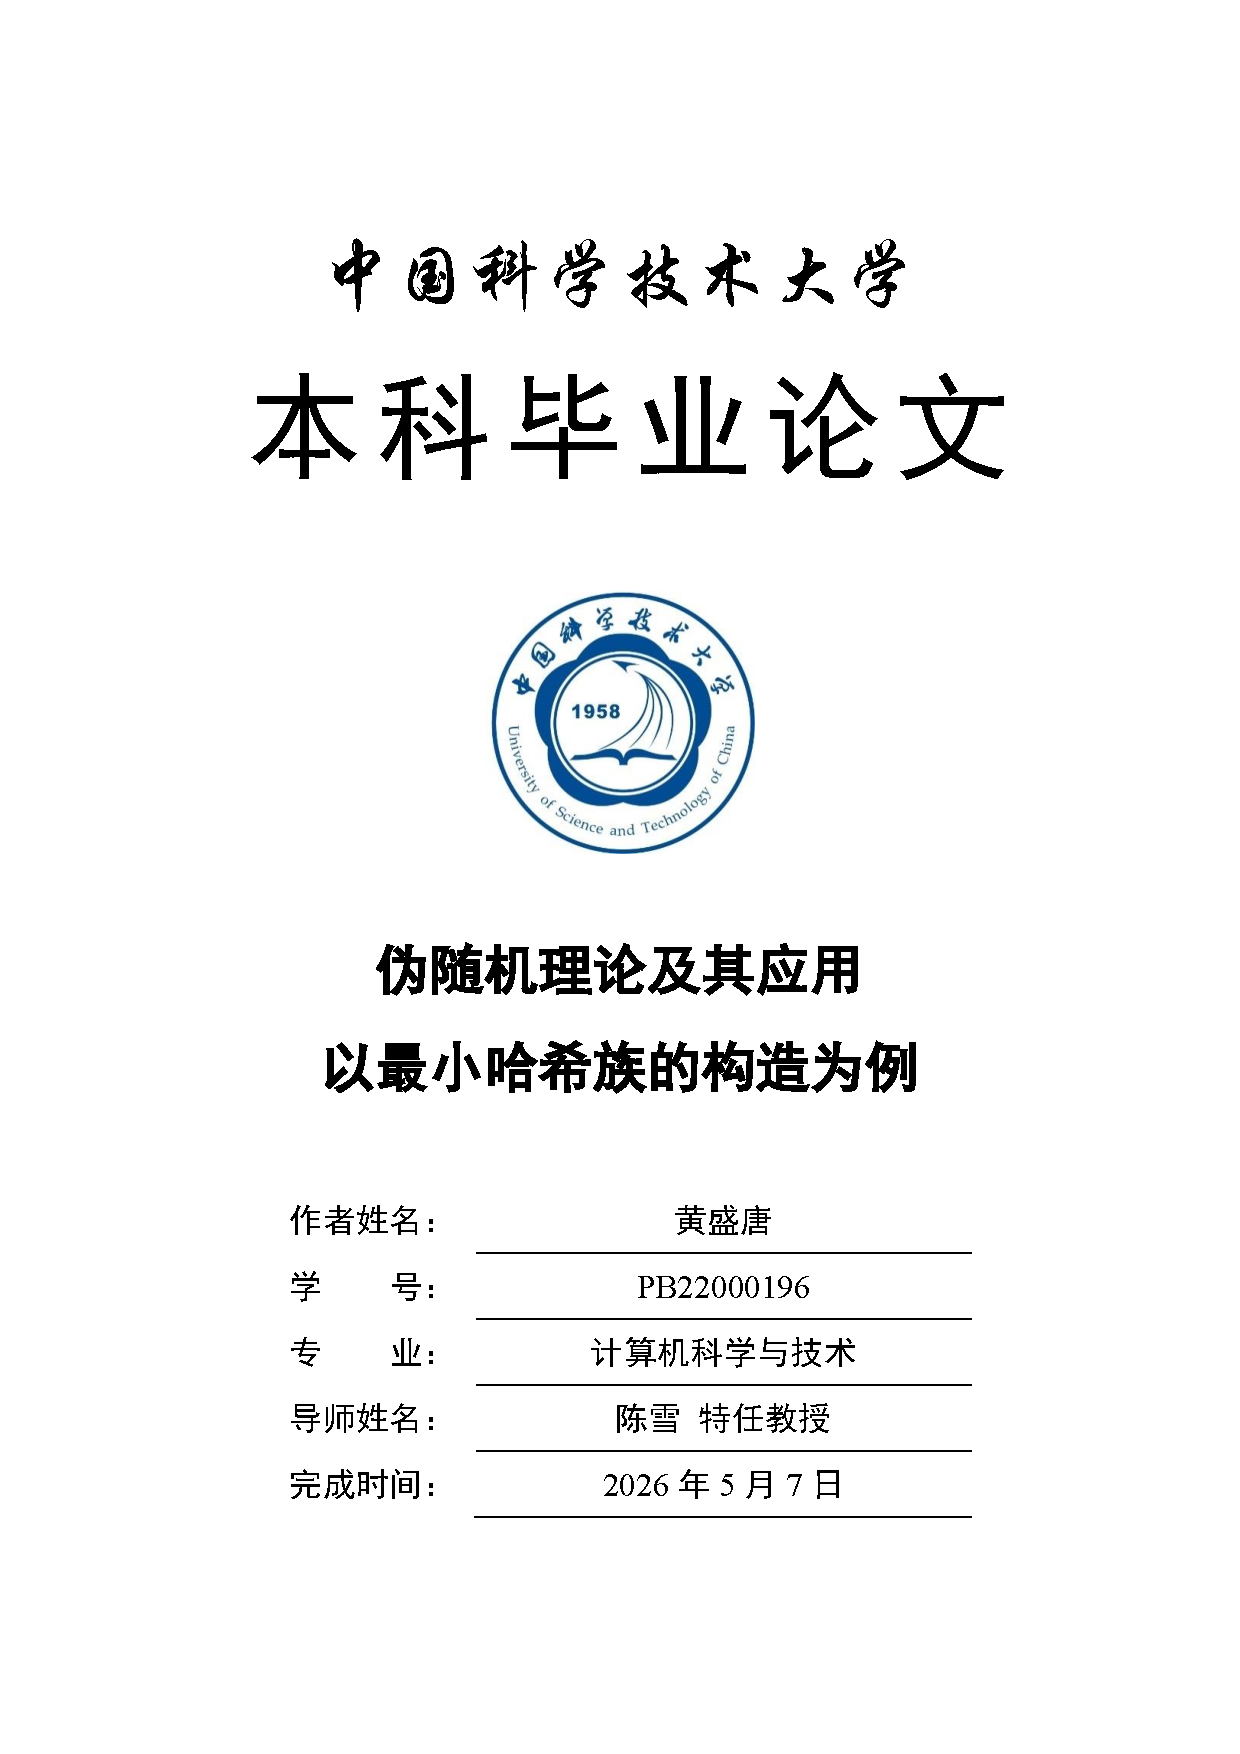
\includepdf[pages=-]{figs/title.pdf} % 预先合成扉页
\newpage

%-------摘要-------
\newpage
\fancyfoot{} % 去除页脚页码

\section*{\zihao{-2}摘要}

随机化已成为计算机科学的核心方法之一，在算法设计、密码学等领域发挥着重要作用。然而，随机性的使用也带来了理论与实践上的挑战，推动了伪随机理论的发展，其目标是在尽量减少随机性的前提下模拟真实随机行为。

作为伪随机理论的重要应用，本文研究最小哈希族及其扩展 $k$-最小哈希族的显式构造问题。粗略地说，最小哈希族保证：对定义域任意固定子集 $X$，经过哈希映射后，其中每个元素以几乎相等概率成为严格最小值；$k$-最小哈希族将此性质推广到 $X$ 中任意大小至多为 $k$ 的子集。该族最经典的应用是近似计算 Jaccard 相似度，在流式算法与图论算法设计中也发挥关键作用。本质上，它是一类具有乘法误差保证的去随机化问题，核心挑战在于保证误差的同时优化随机性使用。

针对上述挑战，本文首次给出使用有限次独立性构造 $k$-最小哈希族所需独立次数的紧界 $\Theta(k + \log 1/\delta)$。进一步，我们给出首个种子长度最优为 $O(\log N)$，且可以实现亚常数乘法误差的显式最小哈希族构造；并将其扩展到 $k$-最小哈希的情形，得到种子长度为 $O(k \log N)$ 的构造。构造方法基于经典的分桶哈希、随机性回收与域缩减，并引入新的均匀性与直和结构，以处理乘法误差与条件概率。

\

\noindent \textbf{关键词：}
最小哈希族；伪随机性；去随机化

\newpage

\section*{\zihao{-2} Abstract}

Randomization has become a core methodology in computer science, playing an important role in algorithm design, cryptography, and other fields. However, the use of randomness also brings theoretical and practical challenges, driving the development of pseudorandomness theory, which aims to simulate truly random behavior while using as little randomness as possible.

As an important application of pseudorandomness, this paper studies the explicit construction of min-wise hash families and their generalization, $k$-min-wise hash families. Roughly speaking, a min-wise hash family guarantees that for any fixed subset $X$ of the domain, after hashing, each element of $X$ is almost equally likely to become the strict minimum; the $k$-min-wise hash family extends this property to any subset of $X$ with size at most $k$. The most classic application is estimating Jaccard similarity, and the families also play a key role in streaming and graph algorithms. In essence, this is a derandomization problem with multiplicative error guarantees, where the core challenge is to minimize randomness usage while controlling the error.

To address this challenge, we provide for the first time a tight bound $\Theta(k + \log 1/\delta)$ on the degree of independence required to construct a $k$-min-wise hash family using bounded independence. Furthermore, we give the first explicit construction of a min-wise hash family with optimal seed length $O(\log N)$ and sub-constant multiplicative error; extending to the $k$-min-wise case, we obtain a construction with seed length $O(k \log N)$. Our construction is based on classical bucket hashing, randomness recycling and domain reduction, and introduces new uniformity and direct sum structures to handle multiplicative error and conditional probabilities.

\

\noindent \textbf{Key Words:}
Min-Wise Hash Family; Pseudorandomness; Derandomization

%-------目录-------

\newpage

\fancyfoot{}
\cfoot{\zihao{-5}\thepage} % 页脚页码

\setcounter{page}{1}

\tableofcontents


%-------正文-------

\newpage
\section{绪论}\label{sec:introduction}

\subsection{研究背景}

\paragraph{伪随机理论.}

随机化方法在理论计算机科学中扮演着极其重要的角色。无论是在算法设计、密码学，还是在组合结构的构造中，引入随机性往往可以显著简化问题并获得更优的性能。例如，在素性测试、多项式同一性测试以及各种图算法问题中，经典的高效算法最初均依赖随机化技术 \cite{Mitzenmacher_Upfal_Probability_and_Computing}。与此同时，随机性也是密码学安全性的核心来源之一 \cite{Goldreich_crypto_book_1,Goldreich_crypto_book_2,GOLDWASSER1984270}。

在组合数学中，随机性还催生了著名的由 Erd\H{o}s 提出的\emph{概率方法}（probabilistic method \cite{The_Probabilistic_Method}）。该方法的基本思想是：如果可以证明一个随机选择的对象以非零概率满足某种性质，则必然存在一个确定性的对象满足该性质。数学家们利用这一方法证明了诸多重要结构的存在性，例如 Ramsey 图等 \cite{Erdos_Ramsey_prob_method}。然而，这类证明通常仅提供存在性结论，而未给出具体构造。更进一步，随机选择的对象往往需要耗费指数时间来寻找，从而在算法上不可行。因此，在组合结构研究和算法应用中，我们更希望得到\emph{显式构造}，即能够在多项式时间内生成的对象。显式性不仅使得这些结构可用于实际计算，还往往揭示其更深层的结构性质。事实上，如何将概率方法中的存在性结果转化为显式构造，是伪随机理论研究的重要驱动力之一。

从算法的角度来看，另一个核心问题是\emph{去随机化}（derandomization）：即能否在不显著损失效率的前提下，将随机算法转化为确定性算法。这一问题在计算复杂性理论中具有基础性地位，集中体现为著名的 $\mathbf{BPP}\text{ vs }\mathbf{P}$ 问题。伪随机生成器（pseudorandom generator）正是研究这一问题的核心工具。直观而言，伪随机生成器试图用一个较短的随机种子生成一个“看起来随机”的长序列，使得任意高效算法都无法区分其输出与真正的均匀分布。若存在能够“欺骗”所有多项式时间算法的高效伪随机生成器，则可以推出 $\mathbf{BPP} = \mathbf{P}$。这一方向的研究已与复杂性理论中的多个核心问题建立了深刻联系，例如电路下界、难度放大等 \cite{Nisan_Wigderson_Hardness_vs_randomness,IW97_worst_case_to_PRG,Yao_PRG}。

然而，由于证明“所有高效算法均无法区分”这一性质本身具有极高难度，目前的研究通常转向考虑\emph{受限计算模型}下的伪随机性。例如，针对空间受限计算（如单次只读分支程序，这与 $\mathbf{BPL}\text{ vs }\mathbf{L}$ 问题有关，与此有关的研究包括但不局限于 \cite{Nisan90_PRG,INW94_PRG,NZ96_Nisan_Zuckerman_PRG,Saks_Zhou_BPL_L_1_5,MRT_width_3_ROBP,Hoza_RANDOM21_L_1_5_sqrt,Cheng_Wu_WPRG}）、各式各样的受限电路类型（如 \cite{Lyu_AC0_PRG,DHH_read_once_DNF_PRG,DHH_iterated_restrictions}）、代数模型（如 \cite{NN93_almost_k_wise,Viola2009_low_degree_poly_PRG}）、或其他各式各样的布尔函数类的伪随机生成器（如 \cite{ABI86_construction_t_wise,NN93_almost_k_wise,INW94_PRG,GMRTV,GKM_Fourier_shape,GY20_PRG_CR_SOTA}），以及在流式算法和数据结构中的应用等（如 \cite{Indyk_PRG_streaming,CRSW_gradually_increased_independence,RWW_Pseudorandom_graph_in_DS,xue_load_balancing}）。这些研究不仅在理论上取得了丰富成果，也在实践中具有重要意义。有关伪随机理论一个较为完整的论述，我们推荐 Vadhan 的综述 \cite{Vadhan12_survey_pseudorandomness}；而专门针对伪随机生成器理论与构造的讲解，则推荐 Hatami 和 Hoza 的综述 \cite{Hatami_Hoza_PRG_survey}。

形式化地，我们采用如下关于伪随机生成器的定义（我们用 $a = b \pm \delta$ 来表示 $a \in [b - \delta, b + \delta]$）。

\begin{restatable}[伪随机生成器 \cite{Blum_Micali_crypto_pseudorandom, Nisan_Wigderson_Hardness_vs_randomness,Yao_PRG}]{definition}{PseudoRandomGenerator}\label{def:PRG}
    给定一有限集合 $D$ 和一族从 $D$ 到 $\{0, 1\}$ 的函数 $\mathcal{F} = \{f : D \to \{0, 1\}\}$，我们称一函数 $G : \{0, 1\}^\ell \to D$ 是误差为 $\varepsilon$ 的 $\mathcal{F}$ 伪随机生成器（pseudorandom generator），若它满足
    $$
    \E_{s \sim \{0, 1\}^\ell}[f(G(s))] = \E_{x \sim D}[f(x)] \pm \varepsilon,\ \forall f \in \mathcal{F},
    $$
    其中 $\ell$ 被称为 $G$ 的种子长度。
\end{restatable}

上述定义从“不可区分性”的角度刻画了伪随机性：伪随机生成器 $G$ 的输出在函数族 $\mathcal{F}$ 看来与真正的随机分布近似一致（误差至多是 $\varepsilon$）。在不同的分析与应用中，$\mathcal{F}$ 对应不同的计算模型，例如所有的多项式算法、空间受限算法或其他测试函数类。

值得注意的是，伪随机生成器与哈希函数族之间存在紧密联系。在许多应用中，哈希函数族所要求满足的随机性性质，可以等价地表述为对某一类判别函数的期望保持性质。形式化地，设
$$
\mathcal{H} = \{h_1, \ldots, h_{|\mathcal{H}|} : [N] \to [M]\}
$$
为一哈希函数族，则可以将其视为一个函数
$$
G : \{0,1\}^{\log |\mathcal{H}|} \to [M]^N,\quad
G(s) = (h_s(1), \ldots, h_s(N)),
$$
其中 $s$ 对应于函数 $h_s \in \mathcal{H}$ 的编号。这样，关于从 $\mathcal{H}$ 中均匀选取函数的随机性分析，可以转化为对 $G(U)$ 的分布性质分析；反之，针对 $[M]^N$ 上分布的判别问题，也可以理解为对哈希函数族的性质要求。这一等价关系在数据结构与算法分析中尤为常见。

\paragraph{最小哈希族.}

最小哈希（min-wise (independent) hashing）由 Broder、Charikar、Frieze 和 Mitzenmacher \cite{BCFM98} 提出，其目标是在一定程度上模拟均匀随机排列的行为。更具体地说，与完全随机排列相比，最小哈希并不试图刻画所有顺序结构，而仅要求与严格最小值相关的概率性质近似均匀，因此是一种对随机排列的局部模拟。在理想情况下，这一性质要求任意元素在集合中成为严格最小值的概率是均匀的（即下面 \cref{def:k_min_wise} 中误差 $\delta = 0$ 的情形）。然而，\cite{BCFM98} 中证明，实现这一完美性质至少需要 $\Omega(N)$ 比特随机性，在实际算法中代价过高。因此，自然的思路是允许一定的误差，从而构造规模更小、可显式描述的哈希函数族。

\begin{definition}[最小哈希族 \cite{BCFM98}]\label{def:k_min_wise}
    设 $\mathcal{H} = \{h : [N] \to [M]\}$ 为一族从 $[N]$ 到 $[M]$ 的哈希函数。若对于任意 $X \subseteq [N]$ 与 $y \in [N] \setminus X$，都有
    $$
    \Pr_{h \sim \mathcal{H}}\left[ h(y) < \min_{x \in X} h(x) \right]
    = \frac{1 \pm \delta}{|X| + 1},
    $$
    则称 $\mathcal{H}$ 是误差为 $\delta$ 的最小哈希族（min-wise hash family）。
    
    进一步地，若对于任意满足 $X \cap Y = \varnothing$ 且 $|Y| \le k$ 的子集 $X, Y \subseteq [N]$，都有
    $$
    \Pr_{h \sim \mathcal{H}}\left[ \max_{y \in Y} h(y) < \min_{x \in X} h(x) \right]
    = \frac{1 \pm \delta}{\binom{|X| + |Y|}{|Y|}},
    $$
    则称其是误差为 $\delta$ 的 $k$-最小哈希族（$k$-min-wise hash family）。
\end{definition}

最小哈希族的核心应用来自集合相似度估计 \cite{BCFM98, CDF+01}。对于两个集合 $A, B \subseteq [N]$，其 Jaccard 相似度为 $|A \cap B| / |A \cup B|$。利用最小哈希，可以通过比较最小哈希值是否相等来估计该相似度：当使用误差为 $\delta$ 的最小哈希族 $\mathcal{H}$ 且值域 $M$ 足够大保证每个哈希函数都是无碰撞时，有
$$
\Pr_{h \sim \mathcal{H}}\left[\min_{a \in A} h(a) = \min_{b \in B} h(b)\right]
= (1 \pm \delta)\cdot \frac{|A \cap B|}{|A \cup B|}.
$$
因此，通过重复采样多个哈希函数，可以以乘法误差近似 Jaccard 相似度。这一经典应用表明，最小哈希天然需要乘法误差控制，而非加法误差。

在此基础上，最小哈希已被广泛应用于大规模数据处理与随机化算法中。例如，在图算法中，可以将节点的邻域或子图结构表示为集合，从而利用最小哈希高效估计图之间的相似性 \cite{MinHash_Graph_Similarity}，并计算图聚类 \cite{MinHash_Clustering}。在流式算法中，最小哈希还被用于 $\ell_0$ 采样 \cite{CF14,McG14} 与草图算法（sketching）\cite{Cohen2016}，其空间复杂度通常与哈希函数族的规模成正比。此外，它也被广泛应用于稀有度近似 \cite{DM02}、网页去重 \cite{Hen06} 以及数据挖掘 \cite{HGKI02, Hen06} 等问题。$k$-最小哈希则被用于处理需要更高独立性的工作 \cite{KNP+17}。

从伪随机性的角度来看，构造最小哈希族等价于构造具有乘法误差的伪随机生成器，其中 $\log |\mathcal{H}|$ 即为种子长度，也对应实际应用中的空间复杂度。因此，如何在保证误差 $\delta$ 的前提下最小化种子长度，是该问题的核心。

现有显式构造中，一条主要技术路线是基于有限次独立性（bounded independence）。Indyk \cite{minwise_Indyk} 证明，当哈希族具有 $O(\log 1/\delta)$ 次独立性时，即可得到误差为 $\delta$ 的最小哈希族；P{\u{a}}tra{\c{s}}cu 与 Thorup \cite{PT_lb_t_wise_min_wise} 进一步证明 $\Omega(\log 1/\delta)$ 次独立性是必要的，从而在该模型下刻画了最小哈希的紧致独立次数需求。对于 $k$-最小哈希族，Feigenblat、Porat 与 Shiftan \cite{minwise_FPS11} 证明，$O(\log 1/\delta + k \log \log 1/\delta)$ 次独立性即可保证误差 $\delta$。

然而，这一方法仍存在两个主要局限。首先，对于 $k$-最小哈希，上述结果给出的所需独立次数的上下界之间仍存在差距。其次，当误差为亚常数 $\delta = o(1)$ 时，由于 $t$ 次独立哈希族需要 $\Theta(t \log NM)$ 比特随机性，该方法无法达到最优的种子长度 $O(\log (NM / \delta))$（对于 $k$-最小哈希则是 $O(k \log NM + \log 1 / \delta)$）。

另一方面，Saks、Srinivasan、Zhou 和 Zuckerman \cite{SSZZ00_connection_CR_min_wise} 首先将最小哈希的构造归约为组合矩形（combinatorial rectangle）的伪随机生成器问题，并基于该规约给出了种子长度为 $O(\log^{3/2} NM)$ 的构造。此后，针对组合矩形的伪随机生成器经历了长期的发展与改进，目前最好的结果是 Gopalan 与 Yehudayoff \cite{GY20_PRG_CR_SOTA} 的构造，这给出了 $O(\log NM \cdot \log \log NM)$ 的最小哈希构造。

然而，这一路线的核心瓶颈在于：最小哈希要求形如 $\delta/|X|$ 的乘法误差，这对应于极小的加法误差。即使 $\delta$ 为常数，当 $|X| = \Omega(N)$ 时，该误差也达到 $1/N$ 量级，使得种子长度必须超过 $O(\log N M)$。因此，尽管该方向在加法误差意义下已取得显著进展，但仍难以直接得到具有最优种子长度的最小哈希族。

\subsection{论文的主要贡献}

本文针对上一节提到的目前最小哈希族显式构造的不足之处，进行探索研究，并解决了如下两个问题：
\begin{itemize}
    \item 证明了基于有限次独立性构造 $k$-最小哈希的紧致独立次数需求。
    
    \item 给出了首个最小哈希族的显式构造，可以在达到最优种子长度 $O(\log N M)$ 的同时，实现亚常数的乘法误差。这一构造也可以扩展到 $k$-最小哈希上。
\end{itemize}

首先是基于有限次独立性的构造，我们证明了为实现误差为 $\delta$ 的 $k$-最小哈希，需要 $\Theta(k + \log 1 / \delta)$ 次独立性。这改进了此前 \cite{minwise_FPS11} 的上界 $O(\log 1 / \delta + k \log \log 1 / \delta)$，并将上下界匹配在了一起。

\begin{theorem}[\ref{sec:bounded_independence} 结果的非形式化描述]\label{thm:bounded_independence_informal}
    基于有限次独立性的构造，为实现误差为 $\delta$ 的 $k$-最小哈希，$\Theta(k + \log 1 / \delta)$ 的独立次数是足够且必要的。
\end{theorem}

接下来则是可以达到最优种子长度 $O(\log N M)$ 的构造。为了表述方便，我们设 $M = \poly(N)$。下面的构造实现了乘法误差 $2^{-O\left( \frac{\log N}{\log \log N} \right)}$，这几乎是多项式小的，除了指数上的 $1 / \log \log N$ 项。

\begin{theorem}[\cref{thm:min_wise_log_seed} 的非形式化描述]\label{thm:min_wise_log_seed_informal}
    给定任意 $N$，存在种子长度为 $O(\log N)$ 且乘法误差为 $2^{-O\left( \frac{\log N}{\log \log N} \right)}$ 的显式最小哈希族构造。
\end{theorem}

这一构造可以扩展到 $k$-最小哈希上，当 $k = \log^{O(1)} N$，可以得到种子长度为 $O(k \log N)$ 的构造，且乘法误差还是可以保持为 $2^{-O\left( \frac{\log N}{\log \log N} \right)}$。

\begin{theorem}[\cref{thm:k_min_wise_klog_seed} 的非形式化描述]\label{thm:k_min_wise_klog_seed_informal}
    给定任意 $N$ 与 $k = \log^{O(1)} N$，存在种子长度为 $O(k \log N)$ 且乘法误差为 $2^{-O\left( \frac{\log N}{\log \log N} \right)}$ 的显式 $k$-最小哈希族构造。
\end{theorem}

值得注意的是，当 $k = \Omega\left( \frac{\log N}{\log \log N} \right)$ 时，基于有限次独立性的构造 \cref{thm:bounded_independence_informal} 实际上就可以在误差是 $2^{-O\left( \frac{\log N}{\log \log N} \right)}$ 时给出最优的种子长度 $O(k \log N)$ 了。所以实际上，\cref{thm:k_min_wise_klog_seed_informal} 在 $k = o\left( \frac{\log N}{\log \log N} \right)$ 时更加有意义。

\subsection{基础记号规定}

我们使用 $[n]$ 表示集合 $\{1, 2, \ldots, n\}$，使用 ${n \choose k}$ 表示组合数。对于一个有限集合 $S$，我们用 $|S|$ 表示其大小。对于三个实数变量 $a, b$ 和 $\delta$，我们用 $a = b \pm \delta$ 来表示 $a$ 和 $b$ 之间的误差不超过 $\delta$，即 $|a - b| \le \delta$。用不带任何下标的对数符号 $\log$ 表示\emph{以 $2$ 为底数的对数}。

我们使用标准渐进符号 $O(\cdot),\Omega(\cdot),\Theta(\cdot),o(\cdot),\omega(\cdot)$ 分别表示渐进上界、下界、紧界以及严格上/下界；若带有下标（如 $O_C(\cdot)$），则表示在该渐进分析中将参数 $C$ 视为常数，隐含常数可依赖于 $C$。在渐进符号中，任何对于常数的对数，都统一用 $\log$ 表示，这是因为由换底公式这只会影响常数。

在本文中，对于函数 $h:[N]\to[M]$，我们将其视为向量 $[M]^N$ 中的一个元素，反之亦然。更一般地，对于一个哈希函数族
$$
\mathcal{H} = \{h_1, \ldots, h_{|\mathcal{H}|} : [N] \to [M]\},
$$
我们将其与一个函数
$$
G : \{0,1\}^{\log |\mathcal{H}|} \to [M]^N
$$
对应，其中 $G(s) = (h_s(1), \ldots, h_s(N))$，$s$ 表示函数在 $\mathcal{H}$ 中的编号。换言之，从 $\mathcal{H}$ 中均匀选取一个哈希函数，等价于从 $\{0,1\}^{\log |\mathcal{H}|}$ 中均匀选取种子并输出 $G(s)$。在后文中，我们将在这两种视角之间自由切换，而不再显式区分。

对于子集 $S \subseteq [N]$，记 $h(S)$ 为其在 $S$ 上的子向量，并定义 $\max h(S):=\max_{x\in S}h(x), \min h(S):=\min_{x\in S}h(x)$，以及事件 $\{h(S)=\theta\} = \{h(x)=\theta,\ \forall x\in S\}$。

对于两个函数 $f, g : [N] \to [M]$，我们定义它们的\emph{加法}为
$$
(f + g)(x) = (f(x) + g(x) - 1) \bmod M + 1.
$$
同样地，对于两个向量 $f, g \in [M]^N$，$f + g$ 表示对应位置的加法。

对于两个哈希函数族 $\mathcal{H}, \mathcal{G}$，定义它们的\emph{直和}（direct sum）为
$$
\mathcal{H} \oplus \mathcal{G} := \{h + g : h \in \mathcal{H},\ g \in \mathcal{G}\}.
$$
在上述对应关系下，若 $\mathcal{H}, \mathcal{G}$ 分别对应函数 $G_1, G_2$，则其直和 $G_1 \oplus G_2$ 对应于函数
$$
G(s_1, s_2) = G_1(s_1) + G_2(s_2).
$$

对于一个有限集合 $\Omega$ 和一个变量 $x$，我们用 $x \sim \Omega$ 来表示 $x$ 是从 $\Omega$ 中均匀随机选取的；一般来说，$x$ 这一类型的变量，其所有可能的取值是有限的，而 $\Omega$ 是所有可能的取值的一个真子集，故我们亦会使用 $x \sim U$ 来表示 $x$ 是从其所有可能的值中均匀随机选取的，和 $x \sim \Omega$ 进行区分。而对于一个分布 $\mathcal{D}$，我们亦用 $x \sim \mathcal{D}$ 来表示 $x$ 是从分布 $\mathcal{D}$ 中选取的。对于一个事件 $A$，我们用 $\mathbf{1}(A)$ 来表示它的示性函数。

给定定义在同一有限集合 $\Omega$ 上的随机变量 $X,Y$，其统计距离（statistical distance）定义为
$$
\dTV(X,Y)
= \max_{S\subseteq \Omega} |\Pr[X\in S]-\Pr[Y\in S]|
= \frac{1}{2}\sum_{\omega\in\Omega} |\Pr[X=\omega]-\Pr[Y=\omega]|.
$$
我们用 $X \approx_\varepsilon Y$ 表示 $\dTV(X,Y)\le\varepsilon$，并称 $X$ 和 $Y$ 是 $\varepsilon$-接近的。此外，我们将反复使用联合界不等式（union bound）：
$$
\Pr\left[\bigcup_{i=1}^n A_i\right]\le \sum_{i=1}^n \Pr[A_i].
$$

\subsection{论文的结构安排}

本文共分为五个章节，系统研究了最小哈希族的显式构造问题，并给出了相关理论结果与构造方法。各章节内容安排如下。

\ref{sec:introduction} 绪论。本章介绍伪随机性研究的基本动机，引出伪随机生成器概念，并作为其具体应用，介绍最小哈希族的问题背景、主要应用、已有构造方法及其局限。最后总结本文的研究目标与主要结果，并给出基本记号。

\ref{sec:bounded_independence} 基于有限次独立性的构造。本章研究有限次独立哈希在构造 $k$-最小哈希时的能力边界，证明了 \cref{thm:bounded_independence_informal}。作为补充，还分析了经典的仿射哈希构造在该问题中的表现，并说明其无法达到高精度乘法误差。

\ref{sec:optimal_seed_length} 具有最优种子长度的构造。本章给出了一个最小哈希族的显式构造，在达到最优种子长度 $O(\log N)$ 的同时，实现亚常数级别乘法误差 $2^{-O\left( \frac{\log N}{\log \log N} \right)}$，并将其推广至 $k$-最小哈希情形，证明了 \cref{thm:min_wise_log_seed_informal} 与 \cref{thm:k_min_wise_klog_seed_informal}。主要技术包括经典的分桶哈希、随机性回收与域缩减，并创新性地引入了新的均匀性与直和结构，以分析乘法误差和条件概率。

\ref{sec:extractor} 随机性提取器。本章研究与最优种子长度构造相关的技术问题，讨论随机性提取器在该框架中的作用。我们构造了一类具有额外均匀性性质的提取器，并进一步分析了“乘法误差提取器”的可实现性，证明其在一般意义下是不可能的，从而说明前述构造方法的必要性。

\ref{sec:summary} 总结与展望。本章总结全文的主要结果与贡献，并讨论当前工作的局限性与未来可能的研究方向，包括进一步优化误差与改进构造的计算时间等问题，以及一些技术讨论。
\newpage
\section{基于有限次独立性的构造}\label{sec:bounded_independence}

有限次独立性（bounded independence）是哈希函数设计与算法去随机化中的一种核心松弛假设，该性质保证了任意不超过 $t$ 个元素的子集在哈希映射下的联合分布与完全随机函数一致。形式上，其定义如下：

\begin{restatable}[$t$ 次独立哈希族 \cite{WC_bounded_independence}]{definition}{BoundedIndependence}\label{def:t_wise_independence}
    一个从定义域 $\mathcal{U}$ 到值域 $\mathcal{R}$ 的哈希函数族 $\mathcal{H}$ 被称为 $t$ 次独立的（$t$-wise independent），如果对于任意 $t$ 个互不相同的输入 $x_1, \dots, x_t \in \mathcal{U}$ 以及任意 $t$ 个输出值 $y_1, \dots, y_t \in \mathcal{R}$，均有
    $$
    \Pr_{h \sim \mathcal{H}}\big[h(x_1)=y_1, \dots, h(x_t)=y_t\big] = |\mathcal{R}|^{-t}.
    $$
\end{restatable}

相比于完全随机哈希需要的 $\Theta(|\mathcal{U}| \cdot \log |\mathcal{R}|)$ 个随机比特，$t$ 次独立哈希族仅需 $\Theta\big(t \cdot (\log |\mathcal{U}| + \log |\mathcal{R}|)\big)$ 个随机比特，并且实现十分简单（具体构造可参见如 Alon、Babai 和 Itai \cite{ABI86_construction_t_wise}），在理论推导与实际系统实现中均具有重要价值。

$t$ 次独立性实际上也是一种伪随机生成器。具体地，它是所有 \emph{$t$-集团函数}的伪随机生成器，并且误差为 $0$。这里的 $t$-集团函数是指所有依赖于至多 $t$ 个输入位置的布尔函数。由于 $t$-集团函数族的大小为 $2^{O(|\mathcal{U}|^t)}$，因此 $t$ 次独立哈希族作为其伪随机生成器的种子长度至少为 $\Omega(t \cdot \log |\mathcal{U}|)$，而上述构造的种子长度也正好匹配了这一下界。

本章聚焦于如何利用有限次独立哈希族来构造 $k$-最小哈希族。我们首先建立独立次数需求的紧致边界：在 \ref{sec:upper_bound} 中，我们证明仅需 $O(k + \log 1 / \delta)$ 次独立性即可将乘法误差控制在 $\delta$ 以内；在 \ref{sec:lower_bound} 中，我们则又反过来证明了 $\Omega(k + \log 1 / \delta)$ 次独立性是不可避免的。最后，在 \ref{sec:affine_hash} 中，我们深入分析一类具体且广泛使用的有限次独立构造——随机仿射哈希族 $h(x) = Ax \oplus b$，揭示其代数结构导致的相关性将不可避免地引入 $\Omega(\log n)$ 的乘法误差，从而无法胜任高精度的 $k$-最小哈希任务。

\subsection{上界的证明}\label{sec:upper_bound}

我们先来证明上界：使用有限次独立性构造 $k$-最小哈希，所需的独立次数至多为 $O(k + \log 1 / \delta)$。该结果改进了 \cite{minwise_FPS11} 的 $O(\log 1 / \delta + k \log \log 1 / \delta)$ 独立次数上界。具体来说，我们要证明如下定理：

\begin{theorem}\label{thm:k_log_1_eps_upper_bound}
    存在常数 $c > 0$，使得如果 $M \ge N / \delta$，则任何从 $[N]$ 到 $[M]$ 的 $c \cdot (k + \log 1 / \delta)$ 次独立哈希族都满足误差为 $3 \delta$ 的 $k$-最小哈希性质。
\end{theorem}

设 $X, Y \subseteq [N]$ 满足 $X \cap Y = \varnothing$，令 $|X| = s$，并且不失一般性只考虑 $|Y| = k$ 的情形。我们用 $\Pr_\ell$ 表示在 $\ell$ 次独立哈希下的概率测度，而不带下标的 $\Pr$ 表示在完全随机哈希下的概率测度。

现在我们考虑 $(\ell + k)$ 次独立性。直接分析联合概率 $\Pr[\max h(Y) < \min h(X \setminus Y)]$ 较为困难，因为 $X, Y$ 中的不同元素的哈希值存在强相关性。为此，我们枚举 $\theta := \max h(Y)$，进行如下概率分解：
$$
\Pr_{\ell + k}[\max h(Y) < \min h(X)] = \sum_{\theta = 1}^M \frac{\theta^k - (\theta - 1)^k}{M^k} \cdot \Pr_\ell[A_\theta],
$$
$$
\Pr[\max h(Y) < \min h(X)] = \sum_{\theta = 1}^M \frac{\theta^k - (\theta - 1)^k}{M^k} \cdot \Pr[A_\theta],
$$
其中 $A_\theta = \{\min h(X) > \theta\}$，我们设其对应的值为 $Z_\theta = \big| h(X) \cap [1, \theta] \big|$。注意对于 $(\ell + k)$ 次独立测度，我们首先枚举 $\max h(Y) = \theta$，这消耗了 $k$ 次独立性。

设定一个阈值 $T = \frac{c \ell M}{s} \in \N$，其中 $c < 1$ 是待确定的常数，并将求和分成两部分：
$$
\Pr_{\ell + k}[\max h(Y) < \min h(X)] = \sum_{\theta \le T - 1} \frac{\theta^k - (\theta - 1)^k}{M^k} \cdot \Pr_\ell[A_\theta] + \sum_{\theta \ge T} \frac{\theta^k - (\theta - 1)^k}{M^k} \cdot \Pr_\ell[A_\theta].
$$

\paragraph{第一部分.}

考虑 $\Pr_\ell[A_\theta]$。我们使用 Bonferroni 不等式：

\begin{lemma}[Bonferroni 不等式]
    设 $A_1, \ldots, A_n$ 为 $n$ 个事件，则有如下不等式：
    $$
    \forall k = 0, 1, \ldots, n,\ \Pr\left[ \bigcap_{i = 1}^n A_i \right]
    \begin{cases}
        \le \sum_{t = 0}^k (-1)^t \sum_{\mathcal{I} \subseteq [n], |\mathcal{I}| = t} \Pr\left[ \bigcap_{j \in \mathcal{I}} \overline{A_j} \right], & k\text{ 是偶数}; \\
        \ge \sum_{t = 0}^k (-1)^t \sum_{\mathcal{I} \subseteq [n], |\mathcal{I}| = t} \Pr\left[ \bigcap_{j \in \mathcal{I}} \overline{A_j} \right], & k\text{ 是奇数}.
    \end{cases}
    $$
\end{lemma}

设 $\ell$ 是偶数，则我们有
$$
\sum_{j = 0}^{\ell - 1} (-1)^j \sum_{X' \subseteq X, |X'| = j} \Pr_\ell[h(X') \subseteq [1, \theta]] \le \Pr_\ell[A_\theta] \le \sum_{j = 0}^\ell (-1)^j \sum_{X' \subseteq X, |X'| = j} \Pr_\ell[h(X') \subseteq [1, \theta]].
$$

因此
$$
\Pr_\ell[A_\theta] = \sum_{j = 0}^{\ell - 2} (-1)^j \sum_{X' \subseteq X, |X'| = j} \Pr_\ell[h(X') \subseteq [1, \theta]] \pm \Delta,
$$
其中误差项 $\Delta$ 为
$$
\begin{aligned}
    \Delta & \le \sum_{j = \ell - 1}^\ell \sum_{X' \subseteq X, |X'| = j} \Pr_\ell[h(X') \subseteq [1, \theta]] \\
     & \le 2 \binom{s}{\ell - 1} \cdot \left( \frac{\theta}{M} \right)^{\ell - 1} \le 2 \left( \frac{\e s \theta}{M (\ell - 1)} \right)^{\ell - 1}.
\end{aligned}
$$

注意上述分析只涉及大小至多为 $\ell$ 的子集；在这种情况下，完全随机概率测度 $\Pr$ 与 $\ell$ 次独立测度 $\Pr_\ell$ 之间没有区别，故上述分析也给出了 $\Pr[A_\theta]$ 的表达式：
$$
\Pr[A_\theta] = \sum_{j = 0}^{\ell - 2} (-1)^j \sum_{X' \subseteq X, |X'| = j} \Pr_\ell[h(X') \subseteq [1, \theta]] \pm \Delta.
$$

结合以上我们得到
$$
\Pr_\ell[A_\theta] = \Pr[A_\theta] \pm 2 \Delta = \Pr[A_\theta] \pm 4 \left( \frac{\e s \theta}{M (\ell - 1)} \right)^{\ell - 1}.
$$

代回到求和中得到
$$
\begin{aligned}
    \sum_{\theta \le T - 1} \frac{\theta^k - (\theta - 1)^k}{M^k} \Pr_\ell[A_\theta] & = \sum_{\theta \le T - 1} \frac{\theta^k - (\theta - 1)^k}{M^k} \cdot \left( \Pr[A_\theta] \pm 4 \left( \frac{\e s \theta}{M (\ell - 1)} \right)^{\ell - 1} \right) \\
     & = \sum_{\theta \le T - 1} \frac{\theta^k - (\theta - 1)^k}{M^k} \Pr[A_\theta] \pm \frac{4 T^k}{M^k} \cdot \left( \frac{\e s T}{M (\ell - 1)} \right)^{\ell - 1}.
\end{aligned}
$$

\paragraph{第二部分.}

再次考虑 $\Pr_\ell[A_\theta]$，这次我们使用集中不等式来界定它。我们直接使用 \cite{Bellare_Rompel_94} 中的尾界。

\begin{restatable}[$t$ 次独立尾不等式，\cite{Bellare_Rompel_94} 中的 引理 2.3]{lemma}{TWiseTailBound}\label{lem:tail_bound_t_wise_BR94}
    设 $t \ge 4$ 为偶数。假设 $X_1, \ldots, X_n$ 是取值于 $[0, 1]$ 的 $t$ 次独立随机变量。令 $X = X_1 + \cdots + X_n$，$\mu = \E[X]$ 且 $A > 0$。则
    $$
    \Pr[|X - \mu| \ge A] \le 8 \cdot \left( \frac{t \mu + t^2}{A^2} \right)^{t / 2}.
    $$
\end{restatable}

这里我们设一个待定的参数 $4 \le \ell' < \ell$，且 $2 \mid \ell'$。使用上面的集中不等式，并假设对所有 $\theta \ge T$ 有 $\E[Z_\theta] \ge \ell'$，则得到
$$
\text{$\Pr_\ell[A_\theta]$ 和 $\Pr[A_\theta]$ 都 } \le 8 \left( \frac{2 \ell' \E[Z_\theta]}{(\E[Z_\theta])^2} \right)^{\ell' / 2} = 8 \left( \frac{2 \ell' M}{\theta s} \right)^{\ell' / 2}.
$$

代回到求和中，我们得到
$$
\begin{aligned}
    \sum_{\theta \ge T} \frac{\theta^k - (\theta - 1)^k}{M^k} \Pr_\ell[A_\theta] & \le \Pr_\ell[A_T] \sum_{\theta \in [T, 2 T]} \frac{\theta^k - (\theta - 1)^k}{M^k} + \Pr_\ell[A_{2 T}] \sum_{\theta \in [2 T, 4 T]} \frac{\theta^k - (\theta - 1)^k}{M^k} + \cdots \\
     & \le 8 \left( \frac{2 \ell' M}{T s} \right)^{\ell' / 2} \cdot \left( \frac{2 T}{M} \right)^k + 8 \left( \frac{2 \ell' M}{2 T s} \right)^{\ell' / 2} \cdot \left( \frac{4 T}{M} \right)^k + \cdots \\
     & = 8 \left( \frac{2 \ell' M}{T s} \right)^{\ell' / 2} \cdot \left( \frac{2 T}{M} \right)^k \cdot \left( 1 + \left( \frac{1}{2} \right)^{\frac{\ell'}{2} - k} + \cdots \right) \\
     & \le 16 \left( \frac{2 \ell' M}{T s} \right)^{\ell' / 2} \cdot \left( \frac{2 T}{M} \right)^k,
\end{aligned}
$$
其中最后一步要求几何级数至多为 $2$，这需要 $\frac{\ell'}{2} - k \ge 1$。

同样的分析适用于完全随机的概率测度 $\Pr$，所以
$$
\sum_{\theta \ge T} \frac{\theta^k - (\theta - 1)^k}{M^k} \Pr_\ell[A_\theta] = \sum_{\theta \ge T} \frac{\theta^k - (\theta - 1)^k}{M^k} \Pr[A_\theta] \pm 32 \left( \frac{2 \ell' M}{T s} \right)^{\ell' / 2} \cdot \left( \frac{2 T}{M} \right)^k.
$$

\paragraph{合并结果.}

将第一部分和第二部分相加，我们得到总误差：
\begin{align*}
    \sum_{\theta = 1}^M \frac{\theta^k - (\theta - 1)^k}{M^k} \Pr_\ell[A_\theta] & = \sum_{\theta = 1}^M \frac{\theta^k - (\theta - 1)^k}{M^k} \Pr[A_\theta] \\
     & \pm \left( \frac{4 T^k}{M^k} \cdot \left( \frac{\e s T}{M (\ell - 1)} \right)^{\ell - 1} + 32 \left( \frac{2 \ell' M}{T s} \right)^{\ell' / 2} \cdot \left( \frac{2 T}{M} \right)^k \right).
\end{align*}

接下来，我们设定具体参数。定义辅助误差 $\delta' = \delta / 2^z$，其中 $z \in \N$ 待定。

令 $\ell' = \ell / 30$（假设 $60 \mid \ell$ 使得 $\ell'$ 为偶数）。再设 $c = 1 / 6$，则 $T = \frac{\ell M}{6 s}$（假设 $6 \mid \ell$ 使得 $T \in \N$）。这可以满足对所有 $\theta \ge T$ 有 $\E[Z_\theta] = \frac{\theta s}{M} \ge \ell'$ 的假设。此外（假设 $\ell \ge 40$），
$$
\frac{\e s T}{M (\ell - 1)} = \frac{\e \ell}{6 (\ell - 1)} < 1/2, \quad \frac{2 \ell' M}{T s} = \frac{2}{5} < \frac{1}{2}.
$$

进一步假设 $\frac{\ell' }{2} \ge \log \frac{32}{\delta'}$ 和 $\ell - 1 \ge \log \frac{4}{\delta'}$，则
$$
\text{总加性误差} \le \frac{T^k}{M^k} \delta' + \frac{(2 T)^k}{M^k} \delta'.
$$

我们考虑如何设置 $z$ 和 $\ell$ 来满足之前的所有约束（总结如下）：
\begin{equation}\label{eq:constraints}
    \begin{cases}
        60 \mid \ell, \ell \ge 120; \\
        \ell \ge 60 k + 60; \\
        \ell \ge 60 (z + \log 1 / \delta + 5).
    \end{cases}
\end{equation}
并且这样的设置可以确保误差项满足
$$
\frac{T^k}{M^k} \delta' \le \frac{(2 T)^k}{M^k} \cdot \frac{\delta}{2^z} \le \frac{(k / \e)^k}{(s + k)^k} \delta \le \frac{\delta}{\binom{s + k}{k}}.
$$

我们只关心 $s \ge k$ 的情形。剩余的情形可以用 $2k$ 次独立哈希族处理，是平凡的。因此可以将要求放宽为
$$
\frac{(2 T)^k}{M^k} \cdot \frac{\delta}{2^z} \le \frac{(k / \e)^k}{(2 s)^k} \delta.
$$
代入 $T = \frac{\ell M}{6 s}$，这等价于
$$
\left( \frac{2 \e}{3} \right)^k \cdot \ell^k \le k^k \cdot 2^z.
$$
取对数得到
\begin{equation}\label{eq:z_ell_relation}
    z \ge k \log \frac{2 \e}{3} + k \log \frac{\ell}{k}.
\end{equation}

令 $L = \lceil \log 1 / \delta \rceil$。我们设 $z = 15 k + L + 5$ 和 $\ell = 60 (z + L + 5)$。展开得 $\ell = 900k + 120L + 600$，这显然满足 \eqnref{eq:constraints} 中的所有约束。

为了验证误差保证，将 $\ell = 900k + 120L + 600$ 代入 \eqnref{eq:z_ell_relation} 的右边，并使用不等式 $\log(1+x) \le 1.45 x\ (x \ge 0)$ 进行界定：
\begin{align*}
    k \log\left( \frac{\ell}{k} \right) &= k \log\left( 900 \cdot \left( 1 + \frac{120L + 600}{900k} \right) \right) \\
    &= k \log 900 + k \log\left( 1 + \frac{120L + 600}{900k} \right) \\
    &\le 9.82 k + k \cdot 1.45 \cdot \left(\frac{120L + 600}{900k}\right) \\
    &\le 9.82 k + 0.194 L + 0.968.
\end{align*}

加上常数项 $k \log(2 \e/3) \le 0.86 k$，\eqnref{eq:z_ell_relation} 的右边严格小于
$$
\text{RHS} \le 0.86 k + 9.82 k + 0.194 L + 0.968 = 10.68 k + 0.194 L + 0.968.
$$

与我们选择的 $z = 15 k + L + 5$ 逐项比较，显然 \eqnref{eq:z_ell_relation} 成立。

\paragraph{收尾.}

现在我们证明了 $\Pr_{\ell + k}[\max h(Y) < \min h(X)]$ 与 $\Pr[\max h(Y) < \min h(X)]$ 之间最多相差 $2 \delta$。最后，我们还需要证明完全均匀随机哈希自动满足误差为 $\delta$ 的 $k$-最小哈希性质。如 Indyk \cite{minwise_Indyk} 所述，当 $M \ge N / \delta$ 时，这一性质成立。以下是严格的证明。

\begin{lemma}\label{lem:k_min_wise_full_random}
    设 $X, Y \subseteq [N]$ 是两个不相交的集合，满足 $|X| = s$ 和 $|Y| = k$。令 $\sigma: [N] \to [M]$ 是一个完全随机函数，则 $Y$ 中的元素严格小于 $X$ 中的元素的哈希值的概率 $P$ 满足
    $$
    \frac{1}{\binom{s + k}{k}} \left( 1 - \frac{s + k}{M} \right) \le P \le \frac{1}{\binom{s+k}{k}},
    $$
    
    特别地，由于 $s+k \le N$，当 $M \ge \frac{N}{\delta}$ 时，误差至多是 $\delta$。
\end{lemma}

\begin{proof}
    精确概率 $P = \Pr_{\sigma}\left[ \max \sigma(Y) < \min \sigma(X) \right]$ 可以如下计算：
    \begin{align*}
        P & = \sum_{\theta = 1}^M \frac{\theta^k - (\theta - 1)^k}{M^k} \left( 1 - \frac{\theta}{M} \right)^s \\
         & = \sum_{\theta = 1}^M \int_{(\theta - 1) / M}^{\theta / M} k x^{k-1} \left( 1 - \frac{\theta}{M} \right)^s \dd x.
    \end{align*}
    
    无哈希碰撞的理想概率由 Beta 积分给出：
    $$
    I = \int_0^1 k x^{k-1} (1-x)^s \dd x = \frac{1}{\binom{s+k}{k}}.
    $$
    
    对于任意 $x \in [(\theta - 1) / M, \theta / M]$，上界 $1 - \theta / M \le 1 - x$ 立即给出
    $$
    P \le \sum_{\theta = 1}^M \int_{(\theta - 1) / M}^{\theta / M} k x^{k-1} (1-x)^s \dd x = I.
    $$
    
    对于下界，我们使用 $1 - \theta / M \ge 1 - x - 1 / M$ 以及凸性不等式：
    $$
    \left( 1 - \frac{\theta}{M} \right)^s \ge (1-x)^s - \frac{s}{M}(1-x)^{s-1}.
    $$
    
    在所有区间上积分这个下界得到
    \begin{align*}
        P & \ge I - \frac{s}{M} \int_0^1 k x^{k-1}(1-x)^{s-1} \dd x \\
         & = I - \frac{s}{M} \cdot \frac{1}{\binom{s + k - 1}{k}} = I \left( 1 - \frac{s + k}{M} \right).
    \end{align*}
    
    结合这些界，我们得到 $I \left( 1 - \frac{s+k}{M} \right) \le P \le I$。这证明了乘法误差被 $(s + k) / M$ 所控制。由于 $X$ 和 $Y$ 是 $[N]$ 的不交子集，$s+k \le N$，这意味着 $\frac{s+k}{M} \le \frac{N}{M}$。因此，如果 $M \ge N / \delta$，误差至多是 $\delta$。
\end{proof}

因此，综合以上所有，与 $1 / \binom{s + k}{k}$ 相比的乘法误差至多为 $3 \delta$，并且 $\ell + k = \Theta(k + \log 1 / \delta)$，这完成了 \cref{thm:k_log_1_eps_upper_bound} 的证明。

\subsection{下界的证明}\label{sec:lower_bound}

在这一节我们继续来探讨下界的论述，证明：使用有限独立哈希族来构造 $k$-最小哈希，所需的独立性次数至少为 $\Omega(k + \log 1 / \delta)$。这和我们上一节得到的上界是相吻合的。

证明分为两步。首先我们证明，任何 $k$-最小哈希严格地至少需要 $k$ 次独立性。为了看出这一点，假设 $X$ 独立均匀分布在 $[0, 1/2)$ 中，而 $Y$ 均匀分布在 $[0, 1)$ 中，但条件是其落入 $[1/2, 1)$ 的元素个数为奇数。这个条件保持了 $Y$ 的 $(k-1)$ 次独立性，然而它却确定性地迫使 $Y$ 中至少有一个元素落入 $[1/2, 1)$。由于 $X$ 的所有元素严格在 $[0, 1/2)$ 中，概率 $\Pr[\max h(Y) < \min h(X)] = 0$，产生 $100\%$ 的乘法误差。

其次，我们将此与 P{\u{a}}tra{\c{s}}cu 和 Thorup \cite{PT_lb_t_wise_min_wise} 为最小哈希建立的下界相结合：

\begin{theorem}[\cite{PT_lb_t_wise_min_wise} 中的定理 3.1]\label{thm:PT_lb_t_wise_min_wise}
    存在一个常数 $c > 0$，对于任意大小为 $n$ 的键集 $X$ 和另一个键 $y$，存在一个 $t$ 次独立的哈希族 $\mathcal{H} = \{h : X \cup \{y\} \to [0, 1)\}$ 使得
    $$
    \Pr_{h \sim \mathcal{H}}[h(y) < \min h(X)] = \frac{1 + 2^{-c t}}{n + 1}.
    $$
\end{theorem}

这个定理本质上要求了，使用有限次独立哈希族来做最小哈希，所需的独立次数至少是 $\Omega(\log 1 / \delta)$。由于 $k$-最小哈希是比标准的最小哈希更强的性质，为了达到乘法误差 $\delta$，它必然继承这个 $\Omega(\log 1 / \delta)$ 次独立性的下界。

结合这两个约束，我们得到 $k$-最小哈希的所需的独立次数下界为 $\Omega(\max\{k, \log 1 / \delta\}) = \Omega(k + \log 1 / \delta)$。

\subsection{随机仿射哈希族}\label{sec:affine_hash}

为具体考察有限次独立哈希族在最小哈希中的应用，我们首先回顾最经典的构造：一维模线性哈希族 $h(x) = (ax + b) \bmod p$。Broder、Charikar、Frieze、Mitzenmacher \cite{BCFM98} 与 P{\u{a}}tra{\c{s}}cu、Thorup \cite{PT_lb_t_wise_min_wise} 已严格证明，此类哈希族在实现最小哈希时，其乘法误差不可避免地达到 $\Omega(\log n)$。本节我们将研究其高维推广形式——随机仿射哈希族 $h(x) = Ax \oplus b$。显然，该高维仿射族是一维经典线性哈希族在多维向量空间上的直接推广，自然涵盖了一维情形的核心结构。我们将证明，即便在更高维度的设定下，随机仿射哈希族用于最小哈希时同样无法避免 $\Omega(\log n)$ 的乘法误差。此外，由于 $k$-最小哈希是比标准最小哈希更强的性质，若哈希族连基础的最小哈希都无法满足，则必然也无法胜任 $k$-最小哈希族的要求。如下定理定量刻画了这一局限性：

\newcommand{\msb}{\mathsf{msb}}

\begin{theorem}\label{thm:min_wise_random_affine_not_good}
    设 $h(x) = Ax \oplus b$ 为从 $\F_2^u$ 到 $\F_2^\ell$ 的随机仿射哈希函数，其中 $\ell = 2u$，$A \sim \F_2^{\ell \times u}$，且 $b \sim \F_2^\ell$。对任意整数 $k \le u - 1$，存在一个大小为 $n = 2^k$ 的集合 $S \subseteq \F_2^u \setminus \{0\}$，使得查询元素 $q = 0$ 有严格最小哈希值的概率满足以下下界：
    $$
    \Pr_{A,b}[h(0) < \min h(S)] \ge (1 - 2^{-u}) \frac{\log n + 1}{4n - 2} = \Theta\left(\frac{\log n}{n}\right).
    $$
\end{theorem}

\begin{proof}
    设 $V \subseteq \F_2^u$ 为一个 $(k+1)$ 维子空间（因为 $k+1 \le u$，故必然存在）。固定一个非零向量 $z \in V$，并定义仿射超平面 $S = \{ x \in V \mid z^\top x = 1 \}$。显然集合 $S$ 的大小为 $2^k = n$ 且不包含 $0$。我们将 $q = 0$ 指定为查询元素。
    
    对任意 $x \in V \setminus \{0\}$，$Ax = 0$ 的概率为 $2^{-\ell} = 2^{-2u}$。对 $V$ 中所有非零元素应用联合界，限制映射 $A|_V$ 为单射的概率为 $\Pr[\mathcal{E}] \ge 1 - 2^{k+1} 2^{-2u} \ge 1 - 2^{-u}$。我们在 $A|_V$ 是单射的这个事件（记作 $\mathcal{E}$）成立的条件下进行分析。在 $\mathcal{E}$ 条件下，$U = A(V) := \{A v : v \in V\}$ 是 $\F_2^\ell$ 中的一个 $(k+1)$ 维子空间。此外，由于 $0 \notin S$ 且 $A|_V$ 是单射，像集 $Y = A(S)$ 严格不包含 $0$。由于 $Y$ 是仿射超平面的单射像，它构成了 $U$ 中由一个非平凡线性约束所定义的仿射超平面。
    
    对任意非零向量 $y \in \F_2^\ell$，令 $\msb(y)$ 表示其最高位 1 的索引。因为在 $\mathcal{E}$ 条件下 $Y$ 中的每个 $y$ 均严格非零，故索引 $\msb(y)$ 是良定义的。事件 $h(0) < \min h(S)$ 等价于在标准字典序下，对所有 $s \in S$ 均有 $b < As \oplus b$。由于 $y = As \neq 0$，该条件成立当且仅当对每个 $y \in Y$ 均有 $b_{\msb(y)} = 0$。令 $\msb(Y) = \{ \msb(y) \mid y \in Y \}$。由于 $b$ 均匀分布且独立于 $A$，在给定 $A$ 的条件下，该事件发生的条件概率恰好为 $2^{-|\msb(Y)|}$。
    
    设 $e_1, \dots, e_{k+1}$ 为通过高斯消元法（列消元）得到的 $U$ 的一组基，满足 $\msb(e_1) < \dots < \msb(e_{k+1})$。定义 $Y$ 的线性约束可表示为 $\sum_{i=1}^{k+1} c_i \alpha_i = 1$，其中 $\alpha_i$ 是 $y = \sum_{i=1}^{k+1} \alpha_i e_i \in U$ 的坐标。如 \cref{rmk:QR_induce_constraint_uniform} 所推导，系数向量 $c = (c_1, \dots, c_{k+1})$ 在 $\F_2^{k+1} \setminus \{0\}$ 上均匀分布。
    
    $y = \sum_{i = 1}^{k + 1} \alpha_i e_i \in U$ 的最高有效位为 $\msb(e_t)$，其中 $t$ 是满足 $\alpha_t = 1$ 的最小索引。因此，索引 $\msb(e_t)$ 属于 $\msb(Y)$ 当且仅当存在一个坐标向量 $\alpha$，其首个非零分量位于第 $t$ 位。这要求方程 $c_t + \sum_{i = t + 1}^{k + 1} c_i \alpha_i = 1$ 关于 $\alpha_{t + 1}, \dots, \alpha_{k + 1}$ 有解，当且仅当 $c_t, \dots, c_{k + 1}$ 不全为零时成立。令 $T = \max \{ i : c_i = 1 \}$，该可解条件恰好等价于 $t \le T$。因此，$|\msb(Y)| = T$。
    
    事件 $T = j$ 要求 $c_j = 1$ 且对所有 $i > j$ 有 $c_i = 0$。在 $\mathcal{E}$ 条件下，其发生的概率为 $\Pr[T = j \mid \mathcal{E}] = \frac{2^{j-1}}{2^{k+1}-1}$。计算条件期望可得
    $$
    \E[2^{-|\msb(Y)|} \mid \mathcal{E}] = \sum_{j=1}^{k+1} \frac{2^{j-1}}{2^{k+1}-1} 2^{-j} = \frac{k+1}{2(2^{k+1}-1)}.
    $$
    
    最后，由全期望公式可得
    $$
    \Pr[h(0) < \min h(S)] \ge \Pr[\mathcal{E}] \cdot \E[2^{-|\msb(Y)|} \mid \mathcal{E}] \ge (1 - 2^{-u}) \frac{k+1}{2(2^{k+1}-1)} = (1 - 2^{-u}) \frac{\log n + 1}{4 n - 2}.
    $$
\end{proof}

\begin{remark}\label{rmk:QR_induce_constraint_uniform}
    线性约束系数 $c$ 的均匀性可直接由高斯消元法下随机矩阵的性质得出。固定 $V$ 的一组基后，单射映射 $A|_V$ 对应于左乘一个均匀随机选取的列满秩矩阵 $W \in \F_2^{\ell \times (k+1)}$。通过在 $\F_2$ 上进行列消元，$W$ 可唯一分解为 $W = E R$，其中 $E \in \F_2^{\ell \times (k+1)}$ 是 $U$ 的唯一标准阶梯形基（其列的 $\msb$ 索引严格递增），而 $R \in \mathrm{GL}(k+1, \F_2)$ 是记录列操作的可逆坐标变换矩阵。由随机矩阵理论可知，$R$ 在一般线性群上均匀分布。对任意映射后的向量 $y = Wx = E(Rx)$，令 $\alpha = Rx$ 为其在基 $E$ 下的坐标。原始约束 $z^\top x = 1$ 可重写为 $((R^{-1})^\top z)^\top \alpha = 1$。令 $c = (R^{-1})^\top z$。由于 $R$ 是均匀随机的可逆矩阵且 $z \neq 0$，向量 $c$ 在 $\F_2^{k+1} \setminus \{0\}$ 上严格均匀分布。
\end{remark}

\subsection{总结}

本章系统研究了利用有限次独立哈希族构造 $k$-最小哈希族的理论边界与具体构造的局限性，主要结论与技术路线可归纳为以下三个方面：

首先，我们确立了有限次独立性与 $k$-最小哈希之间紧致的定量关系。\cref{thm:k_log_1_eps_upper_bound} 的上界证明，与下界分析共同表明，为实现 $k$-最小哈希，$\Theta(k + \log 1 / \delta)$ 次独立性是足够且必要的，完整刻画了独立次数与近似精度之间的最优权衡。在技术层面，上界证明将目标概率按哈希值阈值分解，并分别控制；下界证明则通过构造保持对抗分布，结合 P{\u{a}}tra{\c{s}}cu 与 Thorup \cite{PT_lb_t_wise_min_wise}的经典结果（ \cref{thm:PT_lb_t_wise_min_wise}），完成了必要性论证。这样紧致的上下界结果，大大改进了此前 Feigenblat、Porat 和 Shiftan \cite{minwise_FPS11} 给出的 $O(\log 1 / \delta + k \log \log 1 / \delta)$ 的上界。

其次，我们对随机仿射哈希族这一经典代数构造进行了理论分析。尽管该族在有限域 $\F_2$ 上具备优良的代数性质，\cref{thm:min_wise_random_affine_not_good} 严格证明了其用于最小哈希族时存在 $\Omega(\log n)$ 的固有乘法误差。证明过程中，我们通过高斯消元提取标准阶梯形基，将最小值事件转化为对最高有效位集合大小的精确计数，最终完成误差下界的定量刻画。

本章结果对哈希函数的理论设计与工程选型具有突出意义。一方面，它表明在追求 $k$-最小哈希时，盲目提高哈希族的独立次数不仅浪费存储空间，且在代数构造（如仿射映射）中仍受限于内在的线性相关性；另一方面，紧致的上下界为实际系统中随机源的精简提供了理论依据，即在给定误差容忍度 $\delta$ 与查询规模 $k$ 时，仅需配置 $\Theta(k + \log 1 / \delta)$ 的独立性即可达到所需效果。
\newpage
\section{具有最优种子长度的构造}\label{sec:optimal_seed_length}

上一章中基于有限次独立性的构造，可以得到一个种子长度为 $O(\log 1 / \delta \cdot \log N)$ 的显式最小哈希族。但当乘法误差 $\delta$ 是一个亚常数时，该种子长度就不是最优的 $O(\log (N / \delta))$。另一种方法是使用组合矩形的伪随机生成器，但这种方法不可避免地需要种子长度 $O(\log N \log \log N)$（除非组合矩形伪随机生成器的种子长度被改进到最优 $O(\log N)$），其局限性的具体论述在 \ref{sec:overview}。

我们在本章中将给出一个构造，首次在种子长度是最优 $O(\log N)$ 时，让乘法误差 $\delta$ 可以达到亚常数级别，更具体的，乘法误差是\emph{几乎多项式小的}：$\delta = 2^{-O\left( \frac{\log N}{\log \log N} \right)}$。

\begin{restatable}{theorem}{MinWiseLogSeed}\label{thm:min_wise_log_seed}
    给定足够大的 $N$ 和任意常数 $C = \Omega(1)$，设乘法误差为 $\delta = 2^{-C \cdot \frac{\log N}{\log \log N}}$，而 $M = \poly(N) \ge 4 N / \delta$，则存在一个显式的误差为 $\delta$ 的最小哈希族 $\mathcal{H} = \{h : [N] \to [M]\}$，其种子长度为 $O_C(\log N)$。
\end{restatable}

同样的问题对于 $k$-最小哈希的构造也存在。当 $\delta = o(2^{-k})$ 时，使用 $O(k + \log 1 / \delta)$ 次独立性的构造，种子长度都不是最优的 $O(k \log N + \log 1 / \delta)$。我们的构造也可以扩展到 $k$-最小哈希族上。

\begin{restatable}{theorem}{KMinWiseKLogSeed}\label{thm:k_min_wise_klog_seed}
    给定足够大的 $N$、任意 $k = \log^{O(1)} N$ 和任意常数 $C = \Omega(1)$，设乘法误差为 $\delta = 2^{-C \cdot \frac{\log N}{\log \log N}}$，而 $M = \poly(N) \ge 4 N / \delta$，则存在一个显式的误差为 $\delta$ 的 $k$-最小哈希族 $\mathcal{H} = \{h : [N] \to [M]\}$，其种子长度为 $O_C(k \log N)$。
\end{restatable}

我们的构造使用了众多伪随机中的经典技术，如分桶哈希、建模为单次只读分支程序进行桶间随机性回收，以及 Lu \cite{Lu02_domain_reduction} 的域缩减技术等。此外，我们还提出了一些新的技术框架，如带有一个特殊均匀性性质的随机性提取器，以及将一个函数与单层 Nisan-Zuckerman 伪随机生成器进行直和的想法，以此来处理条件概率与乘法误差。

我们在 \ref{sec:prelim_construction} 中先介绍一些基本理论与记号约定，然后在 \ref{sec:overview} 中详细阐述构造的核心技术路线。最后在 \ref{sec:construction} 与 \ref{sec:extending_to_k_minwise} 中分别给出最小哈希族与 $k$-最小哈希的构造细节与分析，证明 \cref{thm:min_wise_log_seed} 与 \cref{thm:k_min_wise_klog_seed}。

\subsection{记号约定与基本理论}\label{sec:prelim_construction}

本节中我们介绍若干基本理论，并约定一些记号。首先是我们证明中用于建模抽象的两类核心函数。

第一类核心函数是\emph{单次只读分支程序}（read-once branching program），它可以很好地建模空间受限的随机计算模型，在伪随机理论的研究中具有重要地位。在我们这一节可以以它来建模分桶哈希函数的选择过程。

\begin{definition}[单次只读分支程序]\label{def:ROBP}
    字母表 $\Gamma$ 上的宽度为 $w$、长度为 $n$ 的单次只读分支程序（read-once branching program）是一个分层有向图 $M$，该图包含 $n + 1$ 层，每层有 $w$ 个顶点，并具有以下性质：
    \begin{itemize}
        \item 第一层仅包含一个起始节点，且最后一层的顶点标记为 $0$ 或 $1$。

        \item 第 $i$ 层（$0 \le i < n$）的每个顶点 $v$ 都有 $|\Gamma|$ 条指向第 $i + 1$ 层的边，每条边均用 $\Gamma$ 中的一个元素进行标记。
    \end{itemize}

    同时，如上所述的图 $M$ 天然地定义了一个函数 $f_M : \Gamma^n \to \{0, 1\}$：当输入为 $(x_1, \ldots, x_n) \in \Gamma^n$ 时，根据边的标记遍历图，并输出最终到达顶点的标记。我们把这样的函数也叫做单次只读分支程序。
\end{definition}

第二类核心函数是\emph{组合矩形}（combinatorial rectangle），它是单次只读分支程序的一种特殊类型，在各分量上具有独立结构。

\begin{definition}[组合矩形]\label{def:comb_rect}
    给定字母表 $[M]$，我们取其上的任意 $N$ 个子集 $S_1, \ldots, S_N \subseteq [M]$，其组合矩形（combinatorial rectangle）是定义为 $N$ 个集合示性函数的乘积：
    $$
    f(x_1, \ldots, x_N) = \prod_{i = 1}^N \mathbf{1}(x_i \in S_i).
    $$
    等价地，它是由 $N$ 个任意函数 $f_1, \ldots, f_N:[M] \to \{0,1\}$ 定义的函数：
    $$
    f(x_1, \ldots, x_N) = \prod_{i = 1}^N f_i(x_i).
    $$ 
\end{definition}

而为了进行去随机化，我们当然需要构造伪随机生成器（pseudorandom generator），来针对单次只读分支程序和组合矩形。我们在此陈述相关定义，并回顾一些经典结果。首先回顾伪随机生成器本身的定义：

\PseudoRandomGenerator*

构造伪随机生成器的一个基本组件是 $t$ 次独立哈希函数族，其本身也可以视作是误差为 $0$ 的 $t$-集团函数的伪随机生成器。

\BoundedIndependence*

我们的证明中会再一次用到上一章用过的关于 $t$ 次独立性的集中不等式。

\TWiseTailBound*

因为我们的构造是分层的，故在证明中我们会不断切换哈希函数的记号，这时候还用上一节的简略记号 $\Pr_t$ 来表示 $t$ 次独立测度就不合适了。因此，在本章的其余部分，我们用 $\Pr_{\sigma : t\text{-wise}}$ 与 $\E_{\sigma : t\text{-wise}}$ 来表示 $\sigma$ 是 $t$ 次独立函数时的概率测度与期望。

接下来我们陈述有关组合矩形的伪随机生成器的结果。组合矩形的伪随机生成器在过去几十年中得到了广泛研究 \cite{ASWZ96_PRG_rect_comb, LLSZ95,SSZZ00_connection_CR_min_wise, Lu02_domain_reduction, GMRTV, GY20_PRG_CR_SOTA}。目前最新最优的结果，是 Gopalan 和 Yehudayoff \cite{GY20_PRG_CR_SOTA} 给出的：

\begin{theorem}[\cite{GY20_PRG_CR_SOTA} 中的 定理 1.9]\label{thm:PRG_comb_rect}
    对于任意误差 $\varepsilon$、维数 $N$ 和字母表 $[M]$，均存在显式的误差为 $\varepsilon$ 的组合矩形伪随机生成器，其种子长度为
    $$
    O\big(\left( \log (M / \varepsilon) + \log \log N \right) \cdot \log \log (M/\varepsilon)\big).
    $$
\end{theorem}

该定理的一个直接推论是：存在一个种子长度为 $O(\log NM)$ 且误差几乎为多项式级小 $2^{-O\left(\frac{\log NM}{\log \log NM}\right)}$ 的组合矩形伪随机生成器。该结果基于 Lu \cite{Lu02_domain_reduction} 在组合矩形伪随机生成器之间的归约。具体而言，Lu 通过一系列归约构造了组合矩形的伪随机生成器。\cite{Lu02_domain_reduction} 的第 3 章中，Lu 使用 $O(\log (N M / \varepsilon))$ 个随机比特，在误差 $\varepsilon$ 内将原始问题归约到 $[1/\varepsilon^{O(1)}]^{1/\varepsilon^{O(1)}}$ 上的问题。在这一规约后的问题上使用 \cref{thm:PRG_comb_rect}，可以得到一个种子长度为 $O(\log  1/\varepsilon \log \log 1/\varepsilon)$ 的组合矩形伪随机生成器。故若 $\varepsilon = 2^{-O\left(\frac{\log NM}{\log \log NM}\right)}$，种子长度便只有 $O(\log NM)$。

\begin{corollary}\label{cor:almost_poly_small_error}
    对于任意常数 $C$ 和误差 $\varepsilon = 2^{-C \cdot \frac{\log NM}{\log \log NM}}$，均存在一个显式的误差为 $\varepsilon$ 的组合矩形伪随机生成器，其种子长度为 $O_C(\log NM)$。
\end{corollary}

最后我们则来阐述单次只读分支程序的伪随机生成器，最经典的有 Nisan 伪随机生成器 \cite{Nisan90_PRG}、Impagliazzo-Nisan-Wigderson 伪随机生成器 \cite{INW94_PRG}、Nisan-Zuckerman 伪随机生成器 \cite{NZ96_Nisan_Zuckerman_PRG} 等。我们在这里给出\emph{单层 Nisan-Zuckerman 伪随机生成器}的定义与分析结果。首先需要引入随机性提取器（randomness extractor）的概念：

\begin{restatable}[随机性提取器 \cite{NZ96_Nisan_Zuckerman_PRG}]{definition}{Extractor}\label{def:extractor}
    对于一个支撑集为 $\Omega$ 的随机源 $X$，其最小熵定义为
    $$
    \Hmin(X) = \min_{x \in \Omega} \log \left( \frac{1}{\Pr[X = x]} \right).
    $$

    而若 $\Ext : \{0, 1\}^n \times \{0, 1\}^d \to \{0, 1\}^m$ 满足：对于任意最小熵至少为 $k$ 的随机源 $X$，均有 $\Ext(X, U_d) \approx_{\varepsilon} U_m$，则称其为 $(k,\varepsilon)$-提取器（对于任何 $\ell \in \N$，$U_\ell$ 表示 $\{0, 1\}^\ell$ 上的均匀分布）。
\end{restatable}

对于我们最小哈希族的构造，随机性提取器需要有一个额外的特殊性质：对于任何固定的种子 $s$，均有 $\Ext(U_n, s) = U_m$，其证明推迟至 \ref{sec:extractor}。

\begin{restatable}{lemma}{ExtractorUniform}\label{lem:extractor_unif}
    给定任意的 $n$，熵 $k \le n$ 与 $m \ge k / 2$，和任意误差 $\varepsilon$，均存在一个显式的 $(k, \varepsilon)$-提取器 $\Ext : \{0, 1\}^n \times \{0, 1\}^d \to \{0, 1\}^m$，满足 $d = O(\log (n / \varepsilon))$。此外，$\Ext$ 满足一个额外性质：对于任意固定种子 $s \in \{0, 1\}^d$，均有 $\Ext(U_n, s) = U_m$。 
\end{restatable}

下面我们正式阐述单层 Nisan-Zuckerman 伪随机生成器的定义：

\begin{definition}[单层 Nisan-Zuckerman 伪随机生成器]\label{def:NZ_PRG}
    对于 $\{0, 1\}$ 上长度为 $n$、宽度为 $w$ 的单次只读分支程序，以及一个随机性提取器 $\Ext : \{0, 1\}^{3 \log w} \times \{0, 1\}^d \to \{0, 1\}^{\log w}$，设 $\ell = n / \log w$，则单层 Nisan-Zuckerman 伪随机生成器的定义如下：
    $$
    G(x, s_1, \ldots, s_\ell) = \big(\Ext(x, s_1), \Ext(x, s_2), \cdots, \Ext(x, s_\ell)\big).
    $$
\end{definition}

Nisan 和 Zuckerman 基于类似 \cref{lem:extractor_unif} 的显式提取器构造，将如上的单层构造迭代运用若干次，最终得到了一个可以针对长度很短的单次只读分支程序的伪随机生成器。在我们的证明中并不需要这一分析，我们仅将其列于此处以供欣赏参考。

\begin{lemma}[\cite{Hatami_Hoza_PRG_survey} 中的 引理 3.4.9]
    对于任意误差 $\varepsilon$，若 \cref{def:NZ_PRG} 中的 $\Ext$ 是一个 $(2 \log w, \varepsilon / (3 \ell))$-提取器，$d = O(\log (n / \varepsilon))$，并且计算 $\Ext$ 的输出只需要 $O(\log (w / \varepsilon))$ 的空间。则对于 $\{0, 1\}$ 上长度为 $n$、宽度为 $w$ 的单次只读分支程序，$G$ 是一个误差为 $\varepsilon$ 的显式伪随机生成器，并且种子长度为
    $$
    O\left( \log w + \frac{\log (n / \varepsilon)}{\log w} \right).
    $$
    而且更进一步，计算 $G(x, s_1, \ldots, s_\ell)$ 只需要空间 $O(\log (n / \varepsilon))$，并且只需要读取输入 $x, s_1, \ldots, s_\ell$ 一次。
\end{lemma}

\begin{theorem}[Nisan-Zuckerman 伪随机生成器 \cite{NZ96_Nisan_Zuckerman_PRG}]
    设 $\nu > 0$ 和 $c \ge 1$ 是常数。对于任意 $w \in \N$，存在一个显式的伪随机生成器，针对 $\{0, 1\}$ 上宽度为 $w$、长度为 $\log^c w$ 的单次只读分支程序，其种子长度为 $O(\log w)$，误差为 $2^{-\log^{1 - \nu} w}$。
\end{theorem}

\subsection{方法概述}\label{sec:overview}

本节将详细阐述构造显式最小哈希族的核心技术路线。我们的构造可将种子长度压缩至最优的 $O(\log N)$，同时保持次常数级的乘法误差 $\delta = 2^{-O\left(\frac{\log N}{\log \log N}\right)}$。

回顾最小哈希族的定义（可参见 \cref{def:k_min_wise}），其要求对任意集合 $X \subseteq [N]$ 和任意目标元素 $y \in [N] \setminus X$，满足
$$
\Pr_{h \sim \mathcal{H}}[h(y) < \min h(X)] = \frac{1 \pm \delta}{|X| + 1}.
$$
若将哈希族 $\mathcal{H}$ 视为伪随机生成器 $G: \{0,1\}^r \to [M]^N$，则上述条件等价于要求 $G$ 能够以极小的误差模拟均匀哈希的统计行为。与此前相同，我们枚举 $\theta := h(y)$，进行如下概率分解：
\begin{equation}\label{eq:overview_decomp}
\Pr_{h \sim \mathcal{H}}[h(y) < \min h(X)] = \sum_{\theta \in [M]} \Pr_{h \sim \mathcal{H}}[h(y) = \theta \wedge \min h(X) > \theta].
\end{equation}
分解后，示性函数 $\mathbf{1}(h(y) = \theta \wedge \min h(X) > \theta)$ 对于各分量的约束是独立的，这恰好构成一个组合矩形（可参见 \cref{def:comb_rect}）。Saks、Srinivasan、Zhou 和 Zuckerman 的早期工作 \cite{SSZZ00_connection_CR_min_wise} 正是基于此观察，直接调用组合矩形的伪随机生成器进行去随机化。而后 Gopalan 与 Yehudayoff \cite{GY20_PRG_CR_SOTA} 又将参数和构造进行了改进与简化。

然而，这一路径存在根本性障碍：目标乘法误差 $\delta$ 是相对于公平概率 $1/(|X| + 1)$ 而言的，而且和式中一共会累计 $M$ 次加法误差。因此，若要求最终结果具有乘法误差 $\delta$，则每一项允许的加法误差至多为 $\varepsilon = \delta / (M (|X| + 1))$，这使得 $\varepsilon$ 是多项式级别的小量。已知能达到如此小加法误差的组合矩形伪随机生成器都需要 $O(\log N \log \log N)$ 的种子长度（可参见 \cref{thm:PRG_comb_rect}），无法达到 $O(\log N)$ 的最优长度。

为绕过这一从加法误差转换到乘法误差所产生的瓶颈，我们引入“分而治之”的思想。首先，通过一个常数次独立的哈希函数将全集 $[N]$ 随机划分至 $\ell$ 个桶中。设 $y$ 落入第 $j$ 个桶，$X$ 中的元素被分配至各桶 $B_1, \ldots, B_\ell$。根据经典的投球入箱（Balls-into-Bins）模型，以高概率每个桶的大小均约为 $|X|/\ell$。

关键观察在于：若各桶使用相互独立的哈希函数 $\sigma_1, \ldots, \sigma_\ell$，则事件 $\{h(y) = \theta \wedge \min h(X) > \theta\}$ 可严格分解为各桶独立事件的乘积：
\begin{align}
    \Pr_{h \sim \mathcal{H}}[h(y) = \theta \wedge \min h(X) > \theta] = & \Pr_{\sigma_j \sim \mathcal{G}}[\sigma_j(y) = \theta \wedge \min \sigma_j(B_j) > \theta] \notag \\
     & \cdot \prod_{i \ne j} \Pr_{\sigma_i \sim \mathcal{G}}[\min \sigma_i(B_i) > \theta]. \label{eq:bucket_decomp}
\end{align}
此时，每个子问题仅涉及单个桶内的少量元素。由于桶规模显著缩小，我们可用一个规模较小的显式哈希族 $\mathcal{G}$ 来近似每个桶上的均匀哈希行为。只要 $\mathcal{G}$ 足够小，其种子长度 $\log |\mathcal{G}|$ 便合适，且每个子问题的误差也可以控制。

若各桶独立选取哈希函数，总种子长度将为 $\ell \cdot \log |\mathcal{G}|$。为了控制总误差，我们需增大 $\ell$，故该长度仍不可接受。我们希望可以共享桶之间哈希函数选取的随机性，为此，将各桶的选择建模为一个空间受限计算模型——单次只读分支程序（可参见 \cref{def:ROBP}）。具体地，构造一个长度为 $\ell$、宽度为 $2$、输入字母表为 $\mathcal{G}$ 的单次只读分支程序，其第 $i$ 步读取第 $i$ 个桶的哈希函数，状态记录“当前是否已出现 $\le \theta$ 的 $X$ 中元素哈希值”，以及读完第 $j$ 个桶后再记录“$y$ 的哈希值是不是 $\theta$”。

为了压缩种子，我们采用单层 Nisan-Zuckerman 伪随机生成器框架 \cite{NZ96_Nisan_Zuckerman_PRG}。该框架维护一个长度为 $C \log N$ 的公共随机源 $w$，并为每个桶分配一个短种子 $s_1, \ldots, s_\ell$。第 $i$ 个桶的哈希函数由随机性提取器（可参见 \cref{def:extractor}）输出 $z_i = \Ext(w, s_i)$ 索引生成。由于单次只读分支程序的读取是单向的，前序桶对 $w$ 的信息泄露有限，因此单层 Nisan-Zuckerman 伪随机生成器的经典分析表明每个 $z_i$ 仍近似均匀分布。

引入该结构后，\eqnref{eq:bucket_decomp} 的近似形式变为：
\begin{align*}
    \left( \Pr_{\sigma_j \sim \mathcal{G}}[\sigma_j(y) = \theta \wedge \min \sigma_j(B_j) > \theta] \pm \ExtErr \right) \times \prod_{i \ne j} \left( \Pr_{\sigma_i \sim \mathcal{G}}[\min \sigma_i(B_i) > \theta] \pm \ExtErr \right),
\end{align*}
其中 $\ExtErr$ 为提取器引入的加法误差。对于 $i \ne j$ 的普通桶，其概率 $\Pr_{\sigma_i \sim \mathcal{G}}[\min \sigma_i(B_i) > \theta]$ 通常远离 $0$，加法误差 $\ExtErr$ 转化为乘法误差后影响可控。

然而，含目标元素 $y$ 的第 $j$ 个桶面临严峻挑战。不妨假定 $\mathcal{G}$ 是常数次独立的，进而在每个分量的边缘分布都是均匀的，则该桶对应的事件概率满足
$$
\Pr_{\sigma_j \sim \mathcal{G}}[\sigma_j(y) = \theta \wedge \min \sigma_j(B_j) > \theta] \le \Pr_{\sigma_j \sim \mathcal{G}}[\sigma_j(y) = \theta] = 1 / M.
$$
若直接加上提取器误差 $\ExtErr$，在还原为乘法误差时，误差将被放大为 $\ExtErr \cdot M$。由于 $M$ 是多项式大小，而 $\ExtErr$ 为了控制种子长度只能做到 $N^{-o(1)}$，这将彻底破坏乘法误差界。这也正是导致先前方法种子长度无法降至 $O(\log N)$ 的核心症结。

为解决这一瓶颈，我们利用单层 Nisan-Zuckerman 伪随机生成器的两个关键性质：
\begin{enumerate}
    \item \textbf{对称性与顺序无关性：} 单层 Nisan-Zuckerman 伪随机生成器的输出块 $(z_1, \ldots, z_\ell)$ 在结构上是对称的，单次只读分支程序的读取顺序可任意置换而不影响其统计性质。因此，我们可自由调整桶的处理顺序。
    \item \textbf{归纳分析的首项零熵损失：} 单层 Nisan-Zuckerman 伪随机生成器的经典误差分析是归纳进行的。在分析第 $k$ 个输出时，需以第 $1$ 至 $k - 1$ 个输出为条件，此时 $w$ 的条件熵会逐步下降。但\textbf{第一个输出}不需要任何前置条件，此时 $w$ 保持完整的均匀分布，熵无损失。
\end{enumerate}
基于此，我们将含 $y$ 的第 $j$ 个桶\textbf{强制置于单次只读分支程序的第一步读取}。进一步，我们构造一类特殊的提取器，满足以下性质：当输入源 $w$ 服从均匀分布时，对任意固定种子 $s$，输出 $\Ext(w, s)$ 在目标空间 $\mathcal{G}$ 上\textbf{严格服从均匀分布}（而非仅是统计接近）。

这一性质直接导致：第一步（即桶 $j$）的提取误差为 $0$。换言之，$\Pr_{\sigma_j \sim \mathcal{G}}[\sigma_j(y) = \theta \wedge \min \sigma_j(B_j) > \theta]$ 被精确还原，不携带 $\ExtErr$ 项。后续 $\ell-1$ 个桶虽仍引入加法误差，但由于它们不包含 $1/M$ 因子，累积误差经精细分析后可被严格控制在 $o(\delta/M)$ 量级，从而保证总和 \eqnref{eq:overview_decomp} 的乘法误差界。

最后，我们希望可以继续增加桶数 $\ell$，使得总误差更小。但 $\ell$ 很大时，独立生成 $\ell$ 个种子会超出预算。为此，我们调用一个针对组合矩形的伪随机生成器来联合生成单层 Nisan-Zuckerman 伪随机生成器用的 $\ell$ 个种子 $s_1, \ldots, s_\ell$。该伪随机生成器能以 $O(\log N)$ 种子生成高度伪随机的种子向量，我们使用组合矩形伪随机生成器中的域缩减技术，可以使得总误差进一步降至 $2^{-O\left(\frac{\log N}{\log \log N}\right)}$。结合上述分桶乘积展开与首项零误差特性，对 $\theta$ 求和后即可得到定理所述的乘法误差界。

但上述构造直接扩展到 $k$-最小哈希族上会有一点问题。回顾 $k$-最小哈希族的定义（可参见 \cref{def:k_min_wise}），其要求对任何满足 $|Y| \le k$ 与 $X \cap Y = \varnothing$ 的 $X, Y \subseteq [N]$，都有：
$$
\Pr_{h \sim \mathcal{H}}[\max h(Y) < \min h(X)] = \frac{1 \pm \delta}{\binom{|X| + |Y|}{|Y|}}.
$$

不妨只考虑 $|Y| = k > 1$ 的情形。现在 $Y$ 中元素被分配到了指标在 $J := \{g(y) : y \in Y\}$ 中的桶。之前的框架对于不包括 $Y$ 中元素的桶 $B_i\ (i \notin J)$ 还是可以分析得到项 $\Pr_{\sigma_i \sim \mathcal{G}}[\min \sigma_i(B_i) > \theta] \pm \ExtErr$。但对于与 $Y$ 有关的那些桶，如果 $Y$ 中元素被分配到了不同的桶中，即 $|J| > 1$，则之前保证 $\Ext(U, s) = U$ 的提取器没有办法保证所有与 $Y$ 的桶都没有加法误差，之前提到的概率太小导致加法向乘法误差转换爆炸的问题又会出现。

为解决这一新的问题，我们考虑一种直和结构：我们最终的哈希函数是一 $\Theta(k)$ 次独立函数与单层 Nisan-Zuckerman 伪随机生成器的直和。注意到我们使用单层 Nisan-Zuckerman 伪随机生成器，分析若干个事件的合取，实际上是在对一个条件期望链式展开的式子做去随机化：
\begin{align*}
    \Pr_h[\max h(Y) = \theta \wedge \min h(X) > \theta] & =  \Pr_h[ \max h(Y) = \theta \wedge \min h(B_J) > \theta ] \\
     & \cdot \Pr_{\sigma_{i \notin J}}[\min \sigma_i(B_i) > \theta,\ \forall i \notin J \mid \max h(Y) = \theta \wedge \min h(B_J) > \theta].
\end{align*}

因为 $h$ 中包含一个 $\Theta(k)$ 次独立函数，对于与 $Y$ 相关桶的事件，其可以完美地将 $\{\max h(Y) = \theta\}$ 提取出来。同时，又因为单层 Nisan-Zuckerman 伪随机生成器的特性（对于它已经读取过的输出，实际上它只能“记住” $\log w$ 量级的信息），前面与 $Y$ 有关的 $|J|$ 个桶的事件实际上对公用随机源 $w$ 的熵影响不大，具体而言，只会影响至多常数量级。所以对于后续的桶，单层 Nisan-Zuckerman 伪随机生成器的分析仍然适用，可以得到 $\Pr_{\sigma_i \sim \mathcal{G}}[\min \sigma_i(B_i) > \theta] \pm \ExtErr$ 的近似形式。这样就可以保证所有桶的事件都不会引入过大的加法误差，从而保证最终的乘法误差界。

\subsection{具体构造与证明}\label{sec:construction}

本节我们详细描述我们最小哈希族的显式构造，并完成 \cref{thm:min_wise_log_seed} 的证明。先在此重述主定理：

\MinWiseLogSeed*

我们哈希族 $\mathcal{H} = \{h : [N] \to [M]\}$ 的具体构造如下。

\begin{tcolorbox}[breakable]
    \textbf{最小哈希族：种子长度 $O_C(\log N)$，乘法误差 $2^{-C \cdot \frac{\log N}{\log \log N}}$}
    \begin{enumerate}
        \item 设 $\ell := 2^t$，其中 $t := \frac{\log N}{\log \log N}$，并选取足够大的常数 $C_e$、$C_s$ 和 $C_g$ 使得 $C_e > C_s > C_g > C$。
        
        \item 采样一个 $C_g$ 次独立函数 $g : [N] \to [\ell]$，作为将 $[N]$ 分配到 $\ell$ 个桶的分组函数。
    
        \item 应用定理 \cref{thm:PRG_comb_rect} 中的组合矩形伪随机生成器 $\PRG_1$（种子长度为 $O(\log N)$，加法误差为 $2^{- (C_s+C_e) \cdot t - 2}$），生成 $\ell$ 个伪随机种子 $s_1, \ldots, s_\ell \in \{0, 1\}^{C_e \cdot t}$。
        
        \item 采样随机源 $w \sim \{0, 1\}^{C_e \cdot \log N}$，并将 \cref{lem:extractor_unif} 中的 $(0.6 C_e \cdot \log N, \ExtErr)$-提取器 $\Ext : \{0, 1\}^{C_e \cdot \log N} \times \{0, 1\}^{C_e \cdot t} \to \{0,1\}^{0.3 C_e \cdot \log N}$（其中 $\ExtErr = 2^{-C_s \cdot t}$），应用于 $w$ 和 $s_1, \ldots, s_\ell$。对每个 $i \in [\ell]$，令 $z_i := \Ext(w, s_i)$。
        
        \item 定义大小为 $N^{0.3 C_e}$ 的哈希族 $\mathcal{G} = \{ G_1, \ldots, G_{N^{0.3 C_e}} : [N] \to [M] \}$，它是一个从 $[N]$ 到 $[M]$ 的 $(C_s + 1)$ 次独立函数，与 \cref{cor:almost_poly_small_error} 中误差为 $2^{-C_s \cdot t}$ 的组合矩形伪随机生成器 $\PRG_2$ 的直和。
        
        \item 使用 $z_i$ 从 $\mathcal{G}$ 中选取一个函数，记为 $\sigma_i := G_{z_i}$。
        
        \item 最后，对任意 $x \in [N]$，定义哈希函数 $h(x) = \sigma_{g(x)}(x)$。
    \end{enumerate}
\end{tcolorbox}

对于种子长度，分组函数 $g$ 需要 $O(C_g \cdot \log N) = O_C(\log N)$ 的种子长度；组合矩形伪随机生成器 $\PRG_1$ 需要 $O_{C_s, C_e}(\log N) = O_C(\log N)$ 的种子长度；提取器 $\Ext$ 的公用随机源 $w$ 需要 $C_e \cdot \log N = O_C(\log N)$ 的种子长度；哈希族 $\mathcal{G}$ 需要 $O((C_s + C_e) \cdot \log N) + O_{C_s, C_e}(\log N) = O_C(\log N)$ 的种子长度。总的来说，整个构造的种子长度为 $O_C(\log N)$。构造的显式性则是显然的。本节剩余部分我们将着重分析该构造的误差。

\paragraph{分组函数的负载均衡性质.}

首先，从分组函数 $g$ 中可以得到以下性质。为表述方便，在下文中记 $j := g(y)$ 且 $B_i:=\{x \in X : g(x) = i\}$。

\begin{lemma}\label{lem:allocation_small_error}
    设 $C_g$ 是相对于 $C$ 足够大的常数。则 $C_g$ 次独立函数 $g:[N] \rightarrow [\ell]$ 保证：
    \begin{enumerate}
        \item 当 $|X| \le \ell^{0.9}$ 时，以概率 $1 - 1 / \ell^{3 C}$，对所有 $i \in [\ell]$ 有 $|B_i| \le C_g$。

        \item 当 $|X| \in (\ell^{0.9}, \ell^{1.1})$ 时，以概率 $1 - 1 / \ell^{3 C}$，所有桶满足 $|B_i| \le 2 \ell^{0.1}$。
        
        \item 当 $|X| \ge \ell^{1.1}$ 时，以概率 $1-|X|^{-3 C}$，所有桶满足 $|B_i| = (1 \pm 0.1) \cdot |X| / \ell$。
    \end{enumerate}
\end{lemma}

\begin{proof}
    为证明方便，在本证明中设 $r := |X|$。我们分三种情况分别证明。再次强调 $C_g$ 是远大于 $C$ 的常数。
    \begin{enumerate}
        \item 当 $|X| \le \ell^{0.9}$ 时，有
        $$
        \Pr_{g : \text{$C_g$-wise}}[|B_i| \ge C_g] \le {r \choose C_g} \cdot (1 / \ell)^{C_g} \le (r / \ell)^{C_g} \le 1 / \ell^{0.1 C_g} \le 1 / \ell^{3 C + 1},\ \forall i \in [\ell].
        $$
        通过联合界，以概率 $1 - 1 / \ell^{3 C}$，对所有桶有 $|B_i| \le C_g$。

        \item 当 $|X| \in (\ell^{0.9}, \ell^{1.1})$ 时，固定一个桶 $i \in [\ell]$ 并定义 $Z_x := \mathbf{1}(g(x) = i)$。于是 $|B_i| = \sum_{x \in X} Z_x$，且 $\E[|B_i|] = r / \ell$。不妨假设 $C_g \ge 4$ 是偶数，则由 \cref{lem:tail_bound_t_wise_BR94}，有
        \begin{align*}
              & \Pr_{g : \text{$C_g$-wise}}[|B_i| - \E[|B_i|] \ge \ell^{0.1}] \le 8 \left( \frac{C_g \cdot r / \ell + C_g^2}{(\ell^{0.1})^2} \right)^{C_g / 2} \\
            = & \frac{(O_{C_g}(r / \ell))^{C_g / 2}}{\ell^{0.1 C_g}} \le \frac{(O_{C_g}(\ell^{0.1}))^{C_g / 2}}{\ell^{0.1 C_g}} \le \frac{1}{\ell^{3 C + 1}}.
        \end{align*}
        经过联合界，以概率 $1 - 1 / \ell^{3 C}$，对所有 $i$ 有 $|B_i| \le \ell^{0.1} + \E[|B_i|] \le 2 \ell^{0.1}$。

        \item 当 $|X| \ge \ell^{1.1}$ 时。我们有 $r / \ell \ge r^{0.05}$。类似第二种情况的分析，固定 $i \in [\ell]$ 并定义 $Z_x := \mathbf{1}(g(x) = i)$。由 \cref{lem:tail_bound_t_wise_BR94}，有
        \begin{align*}
              & \Pr_{g : \text{$C_g$-wise}}[|B_i| - \E[|B_i|] \ge 0.1 \cdot r / \ell] \le 8 \left( \frac{C_g \cdot r / \ell + C_g^2}{(0.1 \cdot r / \ell)^2} \right)^{C_g / 2} \\
            = & \frac{O_{C_g}(1)}{(r / \ell)^{C_g / 2}} \le \frac{O_{C_g}(1)}{(r^{0.05})^{C_g / 2}} \le \frac{1}{r^{3 C + 1}}.
        \end{align*}
        使用联合界，以概率 $1 - r^{-3 C}$，对每个 $i \in [\ell]$ 有 $|B_i| = (1 \pm 0.1) \cdot r / \ell$。
    \end{enumerate}
\end{proof}

关键在于，由于 $\ell = 2^t = 2^{\frac{\log N}{\log \log N}}$，每种情况的失败概率相对于误差 $\delta / (|X| + 1) = 2^{-C \cdot \frac{\log N}{\log \log N}} / (|X| + 1)$ 都足够小。因此，在证明中，我们可以假设 \cref{lem:allocation_small_error} 中的所有性质均成立，来保证 $B_1, \ldots, B_\ell$ 的良好负载均衡性质。

\paragraph{概率分解为组合矩形.}

接下来我们开始正式分析概率。对于任意的 $X \subseteq [N]$ 与 $y \in [N] \setminus X$，为计算 $\Pr_{h \sim \mathcal{H}}[h(y)<\min h(X)]$，我们将其表示为
\begin{align}
    \Pr_{h \sim \mathcal{H}}[h(y) < \min h(X)] & = \sum_{\theta \in [M]} \Pr_{h \sim \mathcal{H}} [h(y)=\theta \wedge \min h(X)>\theta] \notag \\
      & = \sum_{\theta \in [M]} \E_{g : \text{$C_g$-wise}} \left[\Pr_{w, s_{1 \sim \ell}} \left[ h(y) = \theta \wedge \min h(X) > \theta \right]  \right], \label{eq:minwise_over_theta}
\end{align}
我们的分析将界定 \eqnref{eq:minwise_over_theta} 中的每一项。

\begin{remark}[嵌套期望、固定分组与测度记号约定]
    为简化表述并保证推导严谨，本节统一作如下约定：
    \begin{enumerate}
        \item \textbf{嵌套期望次序：} 形如 $\E_x[\E_y[Z]]$ 的记号严格规定了积分次序：内层期望 $\E_y[\cdot]$ 始终将 $x$ 视为固定参数进行计算，外层再对 $x$ 的分布求期望。此约定贯穿所有条件概率分解与链式展开。因为这里大部分变量都是互相独立的，所以内层不需要是条件期望。

        \item \textbf{固定分组函数 $g$：} 下文分析中，若无特殊提及，均默认 $g$ 已固定（此时 $j=g(y)$ 与各桶 $B_i$ 为确定量，相关事件可建模为单次只读分支程序）。最终概率将利用全期望公式对 $g$ 求和，并由 \cref{lem:allocation_small_error} 保证坏分组函数的贡献可忽略。
        
        \item \textbf{种子采样测度：} 在 $\Pr$ 或 $\E$ 的下标中：$s_{1 \sim \ell}$（不带任何其他描述）表示由 $\PRG_1$ 正常生成；$s_{1 \sim \ell} \sim U$ 表示独立均匀采样；$s_j, s_{i \ne j} \sim U$ 表示仅 $s_j$ 来自 $\PRG_1$，而其余种子替换为独立均匀变量（严格而言，可视为先由 $\PRG_1$ 生成完整序列 $(s'_1,\ldots,s'_\ell)$，仅保留 $s_j = s'_j$，同时独立采样 $s_{i \ne j} \sim U$ 替代其余位置）。若下标仅列出部分种子，则隐含当前事件与未列出的种子独立，其生成方式不影响概率值。
    \end{enumerate}
\end{remark}

\paragraph{组合矩形伪随机生成器的域缩减.}

固定分组函数 $g$ 后，我们只需分析 \eqnref{eq:minwise_over_theta} 中期望符号内部的概率项。回忆 分组 $j := g(y), B_i := \{x \in X : g(x) = i\}$，函数 $\sigma_i := G_{z_i}, z_i := \Ext(w, s_i)$，而最终哈希函数为 $h(x) = \sigma_{g(x)}(x)$，故目标概率可展开为
\begin{align}
      & \Pr_{w, s_{1 \sim \ell}}[h(y) = \theta \wedge \min h(X) > \theta] \notag \\
    = & \Pr_{w, s_{1 \sim \ell}} \left[ (\sigma_j(y) = \theta \wedge \min \sigma_j(B_j) > \theta) \wedge (\min \sigma_i(B_i) > \theta,\ \forall i \ne j) \right] \notag \\
    = & \sum_\alpha \E_w\left[ \Pr_{s_{1 \sim \ell}}\left[ (s_j = \alpha \wedge \sigma_j(y) = \theta \wedge \min \sigma_j(B_j) > \theta) \wedge (\min \sigma_i(B_i) > \theta,\ \forall i \ne j) \right] \right], \label{eq:before_domain_reduction_1}
\end{align}
其中 $\alpha$ 取遍 $\{0, 1\}^{C_e \cdot t}$。

接下来对每个固定的 $w$ 与 $\alpha$ 处理内部的概率。根据条件概率链式法则，原式本应“分解”为
\begin{align*}
     & \Pr_{s_j}[s_j = \alpha \wedge \sigma_j(y) = \theta \wedge \min \sigma_j(B_j) > \theta] \\
     & \cdot \Pr_{s_{1 \sim \ell}}[ \min \sigma_i(B_i) > \theta,\ \forall i \ne j \mid s_j = \alpha \wedge \sigma_j(y) = \theta \wedge \min \sigma_j(B_j) > \theta].
\end{align*}
然而，直接如此写可能面临条件事件 $\{s_j = \alpha \wedge \sigma_j(y) = \theta \wedge \min \sigma_j(B_j) > \theta\}$ 概率为零的退化情形。我们注意到，对于任意固定的 $w$ 与 $\alpha$，事件 $\{s_j = \alpha\}$ 与 $\{\sigma_j(y) = \theta \wedge \min \sigma_j(B_j) > \theta\}$ 的关系仅有两种可能：要么二者互斥，要么 $\{s_j = \alpha\} \subseteq \{\sigma_j(y) = \theta \wedge \min \sigma_j(B_j) > \theta\}$。若互斥，则概率为零，该项对求和无贡献；若严格包含，则 $\{s_j = \alpha\} \wedge \{\sigma_j(y) = \theta \wedge \min \sigma_j(B_j) > \theta\} = \{s_j = \alpha\}$。因此，我们可以安全地将条件简化为仅依赖于 $\{s_j = \alpha\}$（可以证明对于任何固定的 $w$ 和 $\alpha$，有 $\Pr_{s_j}[s_j = \alpha] > 0$，故不会退化，这是由 $\PRG_1$ 的性质保证的，具体可参见 \cref{lem:PRG_CR_LOG} 的证明），即
\begin{align}
    & \Pr_{s_{1 \sim \ell}}\left[ (s_j = \alpha \wedge \sigma_j(y) = \theta \wedge \min \sigma_j(B_j) > \theta) \wedge (\min \sigma_i(B_i) > \theta,\ \forall i \ne j) \right] \notag \\
  = & \Pr_{s_j}[s_j = \alpha \wedge \sigma_j(y) = \theta \wedge \min \sigma_j(B_j) > \theta] \cdot \Pr_{s_{1 \sim \ell}}[ \min \sigma_i(B_i) > \theta,\ \forall i \ne j \mid s_j = \alpha ]. \label{eq:before_domain_reduction_2}
\end{align}

现在考察 \eqnref{eq:before_domain_reduction_2} 中的条件概率项。对于固定的 $w$，第一个事件 $\{\sigma_j(y) = \theta \wedge \min \sigma_j(B_j) > \theta\}$ 因 $s_j = \alpha$ 固定而被确定。对于剩余事件 $\mathbf{1}(\min \sigma_i(B_i) > \theta,\ \forall i \ne j)$，注意到 $\sigma_i = G_{z_i}$ 且 $z_i = \Ext(w, s_i)$，故其构成了关于 $s_1, \ldots, s_\ell$ 的组合矩形。我们利用组合矩形伪随机生成器 $\PRG_1$ 的性质进行域缩减。下面这一引理说明了这一条件概率项，与 $s_{i \ne j}$ 独立均匀选取时的概率，之间的误差至多为 $2^{-C_s \cdot t}$。

\begin{lemma}\label{lem:PRG_CR_LOG}
    由 $\PRG_1$ 生成的随机种子 $s_1, \ldots, s_\ell$ 满足：对任意固定的 $j \in [\ell]$ 与 $\alpha \in \{0, 1\}^{C_e \cdot t}$，以及任意 $\ell$ 个函数 $f_1, \ldots, f_\ell : \{0, 1\}^{C_e \cdot t} \to \{0, 1\}$，有
    $$
    \E_{s_{1 \sim \ell}}\left[ \prod_{i \ne j}f_i(s_i)\ \middle|\ s_j=\alpha \right] = \prod_{i \ne j} \E_{s_i \sim U}[f_i(s_i)] \pm 2^{-C_s \cdot t}.
    $$
\end{lemma}

\begin{proof}
    注意到 $\mathbf{1}(s_j = \alpha)$ 和 $\mathbf{1}(s_j = \alpha) \cdot \prod_{i \ne j} f_i(s_i)$ 都是 $\left( \{0, 1\}^{C_e \cdot t} \right)^\ell$ 中的组合矩形。根据 $\PRG_1$ 的性质，我们有
    $$
    \Pr_{s_j}[s_j = \alpha] = 2^{-C_e \cdot t} \pm 2^{-(C_s + C_e) \cdot t - 2} > 0, \text{\ 以及}
    $$
    $$
    \E_{s_{1 \sim \ell}}\left[ \mathbf{1}(s_j = \alpha) \cdot \prod_{i \ne j} f_i(s_i) \right] = \E_{s_{1 \sim \ell} \sim U}\left[ \mathbf{1}(s_j = \alpha) \cdot \prod_{i \ne j} f_i(s_i) \right] \pm 2^{-(C_s + C_e) \cdot t - 2}.
    $$

    因此可将条件期望表示为
    \begin{align*}
        \E_{s_{1 \sim \ell}}\left[ \prod_{i \ne j}f_i(s_i)\ \middle|\ s_j=\alpha \right] & = \frac{\E_{s_{1 \sim \ell}}\left[ \mathbf{1}(s_j = \alpha) \cdot \prod_{i \ne j}f_i(s_i) \right]}{\Pr_{s_j}[s_j = \alpha]} \\
         & = \frac{\prod_{i \ne j} \E_{s_i \sim U}[f_i(s_i)] \pm 2^{-C_s \cdot t - 2}}{1 \pm 2^{-C_s \cdot t - 2}}.
    \end{align*}

    注意到 $\prod_{i \ne j} \E_{s_i \sim U}[f_i(s_i)] \le 1$，这表明加法误差至多为
    $$
    \frac{\prod_{i \ne j} \E_{s_i \sim U}[f_i(s_i)] + 2^{-C_s \cdot t - 2}}{1 - 2^{-C_s \cdot t - 2}} - \prod_{i \ne j} \E_{s_i \sim U}[f_i(s_i)] \le \left( \frac{1}{1 - 2^{-C_s \cdot t - 2}} - 1 \right) + \frac{2^{-C_s \cdot t - 2}}{1 - 2^{-C_s \cdot t - 2}} \le 2^{-C_s \cdot t}.
    $$

    特别地，我们得到：
    \begin{equation}
        \Pr_{s_{1 \sim \ell}} [ \min \sigma_i(B_i) > \theta,\ \forall i \ne j \mid s_j = \alpha ] = \prod_{i \ne j}\Pr_{s_i \sim U}[\min \sigma_i(B_i) > \theta ] \pm 2^{-C_s \cdot t}. \label{eq:applying_domain_reduction}
    \end{equation}
\end{proof}

将 \eqnref{eq:before_domain_reduction_2} 与 \eqnref{eq:applying_domain_reduction} 代回 \eqnref{eq:before_domain_reduction_1}，并对所有 $\alpha$ 求和。由此可得
\begin{align}
      & \Pr_{w, s_{1 \sim \ell}} \left[ (\sigma_j(y) = \theta \wedge \min \sigma_j(B_j) > \theta) \wedge (\min \sigma_i(B_i) > \theta,\ \forall i \ne j) \right] \notag \\
    = & \sum_\alpha \E_w \left[ \Pr_{s_j} [ s_j = \alpha \wedge \sigma_j(y) = \theta \wedge \min \sigma_j(B_j) > \theta  ] \cdot \left( \prod_{i \ne j}\Pr_{s_i \sim U}[\min \sigma_i(B_i) > \theta] \pm 2^{-C_s \cdot t} \right) \right] \notag \\
    = & \sum_\alpha \Pr_{w, s_j, s_{i \ne j} \sim U}\left[ (s_j = \alpha \wedge \sigma_j(y) = \theta \wedge \min \sigma_j(B_j) > \theta) \wedge (\min \sigma_i(B_i) > \theta,\ \forall i \ne j) \right] \notag \\
      & \pm \sum_\alpha \Pr_{w, s_j}\left[ s_j = \alpha \wedge \sigma_j(y) = \theta \wedge \min \sigma_j(B_j) > \theta \right] \cdot 2^{-C_s \cdot t} \notag \\
    = & \Pr_{w, s_j, s_{i \ne j} \sim U}\left[ (\sigma_j(y) = \theta \wedge \min \sigma_j(B_j) > \theta) \wedge (\min \sigma_i(B_i) > \theta,\ \forall i \ne j) \right] \label{eq:domain_reduction_result} \\
      & \pm \Pr_{w, s_j}\left[ \sigma_j(y) = \theta \wedge \min \sigma_j(B_j) > \theta \right] \cdot 2^{-C_s \cdot t}. \label{eq:domain_reduction_error}
\end{align}

\paragraph{单层 Nisan-Zuckerman 伪随机生成器的连乘积分析.}

经过组合矩形伪随机生成器的域缩减，我们已成功将除 $s_j$ 之外的所有种子替换为独立均匀分布。现在我们利用单层 Nisan-Zuckerman 伪随机生成器框架与 \cref{lem:extractor_unif} 中提取器 $\Ext$ 的特殊性质，分析域缩减后的主体部分 \eqnref{eq:domain_reduction_result}。

给定固定的分组函数 $g$ 与阈值 $\theta$，考虑一个宽度为 $2$、长度为 $\ell$ 的单次只读分支程序，其输入字母表对应提取器输出 $z_1, \ldots, z_\ell$，计算的是如下 $\ell$ 个事件的合取：
$$
( \sigma_j(y) = \theta \wedge \min \sigma_j(B_j) > \theta ) \wedge (\min \sigma_1(B_1) > \theta) \wedge \cdots \wedge (\min \sigma_\ell(B_\ell) > \theta),
$$
其中 $\sigma_i := G_{z_i},\ \forall i \in [\ell]$。

利用单层 Nisan-Zuckerman 伪随机生成器的对称性，我们调整输入读取顺序，使第 $j$ 个桶对应的 $z_j$ 作为第一个输入被读取，其余输入按原顺序紧随其后。记重排后的事件序列为 $A_1, \ldots, A_\ell$，其中 $A_1 = \{ \sigma_j(y) = \theta \wedge \min \sigma_j(B_j) > \theta \}$，$A_2, \ldots, A_\ell$ 依次对应其余桶满足 $\min \sigma_i(B_i) > \theta$ 的条件。此时 \eqnref{eq:domain_reduction_result}可重写为
$$
\Pr_{w, s_j, s_{i \ne j} \sim U}\left[ (\sigma_j(y) = \theta \wedge \min \sigma_j(B_j) > \theta) \wedge (\min \sigma_i(B_i) > \theta,\ \forall i \ne j) \right]
$$
\begin{equation}
    = \Pr_{w, s_j, s_{i \ne j} \sim U}\left[ A_1 \wedge A_2 \wedge \cdots \wedge A_\ell \right]. \label{eq:robp_joint}
\end{equation}

首先分析 $A_1$。由于 $w$ 服从均匀分布且与 $s_j$ 独立，根据 \cref{lem:extractor_unif} 中提取器 $\Ext$ 的额外性质，提取器输出 $z_j = \Ext(w, s_j)$ 在目标空间上严格服从均匀分布。因此第一个函数 $\sigma_j = G_{z_j}$ 完全等价于从 $\mathcal{G}$ 中均匀采样，不引入任何提取器误差：
$$
\Pr_{w, s_j, s_{i \ne j} \sim U}[A_1] = \Pr_{\sigma \sim \mathcal{G}}[\sigma(y) = \theta \wedge \min \sigma(B_j) > \theta].
$$

接下来对剩余事件进行归纳分析。设第 $\beta$ 步读取的桶指标为 $i_\beta$（满足 $i_1 = j$ 且 $\{i_2, \ldots, i_\ell\} = [\ell] \setminus j$）。类似于单层 Nisan-Zuckerman 伪随机生成器的分析，对每个 $\beta = 2, 3, \ldots, \ell$ 分两种情况讨论：
\begin{itemize}
    \item 若 $\Pr_{w, s_j, s_{i \ne j} \sim U}[A_1 \wedge \cdots \wedge A_{\beta - 1}] \ge 2^{-0.4 C_e \cdot \log N}$，考虑条件于 $A_1 \wedge \cdots \wedge A_{\beta - 1}$ 下 $w$ 的分布。该条件仅使 $w$ 每个取值的概率增加至多 $2^{0.4 C_e \cdot \log N}$ 倍，因此该条件分布的最小熵仍至少为 $0.6 C_e \cdot \log N$。由提取器的性质，我们有
    $$
    \Pr_{w, s_j, s_{i \ne j} \sim U}[A_\beta \mid A_1 \wedge \cdots \wedge A_{\beta - 1}] = \Pr_{z_{i_\beta} \sim U}[A_\beta] \pm \ExtErr = \Pr_{\sigma \sim \mathcal{G}}[\min \sigma(B_{i_\beta}) > \theta] \pm \ExtErr.
    $$

    因此
    \begin{align*}
        \Pr_{w, s_j, s_{i \ne j} \sim U}[A_1 \wedge \cdots \wedge A_\beta] & = \Pr_{w, s_j, s_{i \ne j} \sim U}[A_1 \wedge \cdots \wedge A_{\beta - 1}] \cdot \Pr_{w, s_j, s_{i \ne j} \sim U}[A_\beta \mid A_1 \wedge \cdots \wedge A_{\beta - 1}] \\
         & = \Pr_{w, s_j, s_{i \ne j} \sim U}[A_1 \wedge \cdots \wedge A_{\beta - 1}] \cdot \left( \Pr_{\sigma \sim \mathcal{G}}[\min \sigma(B_{i_\beta}) > \theta] \pm \ExtErr \right).
    \end{align*}

    \item 若 $\Pr_{w, s_j, s_{i \ne j} \sim U}[A_1 \wedge \cdots \wedge A_{\beta - 1}] < 2^{-0.4 C_e \cdot \log N}$，则直接意味着
    $$
    \Pr_{w, s_j, s_{i \ne j} \sim U}[A_1 \wedge \cdots \wedge A_\beta] \le 2^{-0.4 C_e \cdot \log N}.
    $$
\end{itemize}

综合两种情况，前 $\beta$ 个事件被接受的概率可写为
\begin{align*}
    \Pr_{w, s_j, s_{i \ne j} \sim U}[A_1 \wedge \cdots \wedge A_\beta] = & \Pr_{w, s_j, s_{i \ne j} \sim U}[A_1 \wedge \cdots \wedge A_{\beta - 1}] \\
     & \cdot \left( \Pr_{\sigma \sim \mathcal{G}}[\min \sigma(B_{i_\beta}) > \theta] \pm \ExtErr \right) \pm 2^{-0.4 C_e \cdot \log N}.
\end{align*}

通过对 $\beta$ 进行归纳 展开，\eqnref{eq:robp_joint} 中的概率可表示为
$$
\Pr_{\sigma \sim \mathcal{G}}\left[ \sigma(y) = \theta \wedge \min \sigma(B_j) > \theta \right] \cdot \prod_{i \ne j} \left( \Pr_{\sigma \sim \mathcal{G}}\left[ \min \sigma(B_i) > \theta \right] \pm \ExtErr \right) \pm \ell \cdot N^{-0.4 C_e}. 
$$

最后，利用 $\mathcal{G}$ 的 $(C_s + 1)$ 次独立性，及其作为组合矩形伪随机生成器的性质（误差为 $2^{-C_s \cdot t}$），我们有
$$
\Pr_{\sigma \sim \mathcal{G}}[\sigma(y) = \theta \wedge \min \sigma(B_j) > \theta] = \frac{1}{M} \Pr_{\sigma : C_s\text{-wise}}[\min \sigma(B_j) > \theta],
$$
且对 $i \ne j$，
$$
\Pr_{\sigma \sim \mathcal{G}}[\min \sigma(B_i) > \theta] \pm \ExtErr = (1 - \theta / M)^{|B_i|} \pm 2^{-C_s \cdot t} \pm \ExtErr = (1 - \theta / M)^{|B_i|} \pm 2 \cdot 2^{-C_s \cdot t}.
$$
代入上述乘积式，即得 \eqnref{eq:domain_reduction_result} 的完整展开：
\begin{align}
      & \Pr_{w, s_j, s_{i \ne j} \sim U}\left[ (\sigma_j(y) = \theta \wedge \min \sigma_j(B_j) > \theta) \wedge (\min \sigma_i(B_i) > \theta,\ \forall i \ne j) \right] \notag \\
    = & \frac{1}{M} \Pr_{\sigma : C_s\text{-wise}}[\min \sigma(B_j) > \theta] \cdot \prod_{i \ne j} \left( (1 - \theta / M)^{|B_i|} \pm 2 \cdot 2^{-C_s \cdot t} \right) \pm \ell \cdot N^{-0.4 C_e}. \label{eq:final_product_expansion}
\end{align}

\paragraph{误差项分析与汇总.}

我们最后要将域缩减的主项 \eqnref{eq:domain_reduction_result} 与误差项 \eqnref{eq:domain_reduction_error} 对所有阈值 $\theta \in [M]$ 及分组函数 $g$ 求和，以此界定最后结果。

对于主项 \eqnref{eq:domain_reduction_result}，我们已经将其化为了 \eqnref{eq:final_product_expansion}，其关于 $\theta$ 与 $g$ 的求和分析计算较为复杂繁琐，且与本文核心构造逻辑无关。为保持行文连贯，我们将主项求和的完整证明移至 \ref{sec:omitted_calculation}。此处仅陈述结论：

\begin{restatable}{lemma}{MinWiseMainTermSummation}\label{lem:minwise_main_term_summation}
    我们有：
    \begin{align*}
          & \sum_{\theta \in [M]} \E_{g : \text{$C_g$-wise}} \left[ \Pr_{w, s_j, s_{i \ne j} \sim U}\left[ (\sigma_j(y) = \theta \wedge \min \sigma_j(B_j) > \theta) \wedge (\min \sigma_i(B_i) > \theta,\ \forall i \ne j) \right]  \right] \\
        = & \sum_{\theta \in [M]} \E_{g : \text{$C_g$-wise}} \left[ \frac{1}{M} \Pr_{\sigma : C_s\text{-wise}}[\min \sigma(B_j) > \theta] \cdot \prod_{i \ne j} \left( (1 - \theta / M)^{|B_i|} \pm 2 \cdot 2^{-C_s \cdot t} \right) \pm \ell \cdot N^{-0.4 C_e} \right] \\
        = & (1 \pm 2^{-2.5 C \cdot t}) \cdot \Pr_{\sigma \sim U}[\sigma(y) < \min \sigma(X)] \pm \frac{2^{-2.5 C \cdot t}}{|X| + 1} = \frac{1 \pm (\delta / 2 + 2^{-2 C \cdot t})}{|X| + 1}.
    \end{align*}
\end{restatable}

接下来重点处理误差项。固定 $g$ 后，同此前对关键桶 $B_j$ 事件 $A_1$ 的分析，有
$$
\Pr_{w, s_j}\left[ \sigma_j(y) = \theta \wedge \min \sigma_j(B_j) > \theta \right] = \Pr_{\sigma \sim \mathcal{G}}[\sigma(y) = \theta \wedge \min \sigma(B_j) > \theta],
$$
故其对 $\theta$ 求和可精确还原为关键桶的最小值事件：
$$
\sum_{\theta \in [M]} \Pr_{w, s_j}\left[ \sigma_j(y) = \theta \wedge \min \sigma_j(B_j) > \theta \right] \cdot 2^{-C_s \cdot t} = \Pr_{\sigma \sim \mathcal{G}}[\sigma(y) < \min \sigma(B_j)] \cdot 2^{-C_s \cdot t}.
$$
由构造可知，$\mathcal{G}$ 包含一个 $(C_s + 1)$ 独立哈希族。根据 Indyk 的经典结论 \cite{minwise_Indyk}（也即本文中的 \cref{thm:k_log_1_eps_upper_bound} 取 $k = 1$ 的特殊情形），该独立族本身即构成常数误差的最小哈希族。故存在绝对常数 $C_0$，使得
$$
\Pr_{\sigma : (C_s + 1)\text{-wise}}[\sigma(y) < \min \sigma(B_j)] \le \frac{C_0}{|B_j| + 1}.
$$

现对所有 $g$ 取期望，并利用 \cref{lem:allocation_small_error} 分情况讨论 $|X|$ 的量级：
\begin{itemize}
    \item 当 $|X| \le 2^{0.5 C_s \cdot t} - 1$ 时，我们直接就有：
    $$
    \Pr_{\sigma : (C_s + 1)\text{-wise}}[\sigma(y) < \min \sigma(B_j)] \cdot 2^{-C_s \cdot t} \le 2^{-C_s \cdot t} \le \frac{2^{-0.5 C_s \cdot t}}{|X| + 1}.
    $$

    所以这时候误差项对乘法误差的贡献不超过 $2^{-0.5 C_s \cdot t} \le 2^{-2 C \cdot t}$。

    \item 当 $|X| \ge 2^{0.5 C_s \cdot t} \ge \ell^{1.1}$ 时，\cref{lem:allocation_small_error} 保证以概率 $1 - 1 / |X|^{3 C}$，对于所有 $i$ 都有 $|B_i| = (1 \pm 0.1) \cdot |X| / \ell$。因此，当分组函数 $g$ 是好的时候，有
    $$
    \Pr_{\sigma : (C_s + 1)\text{-wise}}[\sigma(y) < \min \sigma(B_j)] \cdot 2^{-C_s \cdot t} \le \frac{C_0}{(1 - 0.1) \cdot |X| / \ell} \cdot 2^{-C_s \cdot t} = \frac{O(1) \cdot 2^{-(C_s - 1) \cdot t}}{|X| + 1}.
    $$

    而坏的分组函数 $g$ 则至多贡献
    $$
    \frac{1}{|X|^{3 C}} \le \frac{|X|^{-2 C}}{|X| + 1} \le \frac{(\ell^{1.1})^{-2 C}}{|X| + 1} = \frac{2^{-2.2 C \cdot t}}{|X| + 1}.
    $$
    
    综合起来，这种情况下误差项对乘法误差的贡献不超过 $O(1) \cdot 2^{-(C_s - 1) \cdot t} + 2^{-2.2 C \cdot t} \le 2^{-2 C \cdot t}$。
\end{itemize}

综合主项与误差项界定，我们最终得到乘法误差至多是 $\delta / 2 + 2^{-2 C \cdot t} + 2^{-2 C \cdot t} \le \delta = 2^{-C \cdot \frac{\log N}{\log \log N}}$，完成证明。

\subsection{往 $k$-最小哈希族的扩展}\label{sec:extending_to_k_minwise}

在本节中我们将构造扩展到 $k$-最小哈希族上，完成 \cref{thm:k_min_wise_klog_seed} 的证明。定理重述如下：

\KMinWiseKLogSeed*

由于 $k$-最小哈希族构造与上一节中的最小哈希族构造在整体框架上高度相似，我们将仅对两者的差异部分进行详细说明。对于与上一节较为相似的部分，我们将省略若干推导细节甚至直接给出结论而不证明。

首先是哈希族 $\mathcal{H} = \{h : [N] \to [M]\}$ 的具体构造：

\begin{tcolorbox}[breakable]
    \textbf{$k$-最小哈希族：$k = \log^{O(1)} N$，种子长度 $O_C(k \log N)$，乘法误差 $2^{-C \cdot \frac{\log N}{\log \log N}}$}

    \begin{enumerate}
        \item 设 $\ell := 2^{t}$，其中 $t := \frac{\log N}{\log \log N}$，并选取足够大的常数 $C_e$、$C_s$ 和 $C_g$ 满足 $C_e > C_s > C_g > C$。
        
        \item 采样一个 $C_g \cdot k$ 次独立函数 $g : [N] \to [\ell]$，作为将 $[N]$ 分配到 $\ell$ 个桶中的分组函数。
        
        \item 应用 \cref{thm:PRG_comb_rect} 中的组合矩形伪随机生成器 $\PRG_1$，其种子长度为 $O_C(k \log N)$，可以生成 $\ell$ 个种子 $s_1, \ldots, s_{\ell}$，每个种子长度为 $C_e \cdot t$，误差为 $2^{-(C_s+C_e) \cdot t \cdot k - 2}$。
        
        \item 采样一个随机源 $w \sim \{0, 1\}^{k \cdot C_e \log N}$，并应用 \cref{lem:extractor_unif} 中的 $(0.6 k \cdot C_e \log N, \ExtErr)$-提取器 $\Ext:\{0, 1\}^{k \cdot C_e \log N} \times \{0, 1\}^{C_e \cdot t} \to \{0, 1\}^{C_e \cdot \log N}$，其中误差为 $\ExtErr = 2^{-C_s \cdot t}$，将 $w$ 与 $s_1, \ldots, s_\ell$ 作为输入：令 $z_i := \Ext(w, s_i), \forall i \in [\ell]$。
        
        \item 设 $\sigma_i := \PRG_2(z_i)$，其中 $\PRG_2$ 是 \cref{cor:almost_poly_small_error} 中的组合矩形伪随机生成器，误差为 $2^{-C_s \cdot t}$。
        
        \item 对于每个 $x \in [N]$，定义 $\varphi(x) := \sigma_{g(x)}(x)$。
        
        \item 采样一个 $(C_e + 1) \cdot k$ 次独立哈希函数 $\psi : [N] \to [M]$。
            
        \item 最后的哈希函数被定义为两个部分加起来 $h := \varphi + \psi$。实际上，假设 $\psi$ 是从 $(C_e + 1) \cdot k$ 次独立哈希函数族 $\Psi$ 得来的，而 $\varphi$ 的构造对应另一个哈希函数组 $\Phi$，那么最后的哈希函数族被定义为这两个的直和 $\mathcal{H} := \Phi \oplus \Psi$。
    \end{enumerate}
\end{tcolorbox}

值得注意的是 $k = \log^{O(1)} N$ 是为了保证第三步中的 $\PRG_1$ 的种子长度为 $O_C(k \log N)$，从而使得整体构造的种子长度仍为 $O_C(k \log N)$。

对于误差分析，我们首先关注的还是分组函数 $g$ 的性质。我们设 $J := \{g(y) : y \in Y\}$，$B_i := \{g(x) : x \in X\},\ \forall i \in [\ell]$，而 $B_J := \bigcup_{j \in J} B_j$。下面引理的证明与 \cref{lem:allocation_small_error} 高度相似，我们省略细节的论证。

\begin{restatable}{lemma}{AllocationKMinWise}\label{lem:allocation_k_min_wise}
    设 $C_g$ 是相较于 $C$ 足够大的常数。则分组函数 $g$ 满足：
    \begin{enumerate}
        \item 当 $|X| \le \ell^{0.9}$ 时，以概率 $1 - \frac{1}{\ell^{3 C} \cdot |X|^{k}}$，对于所有 $i \in [\ell]$ 都有 $|B_i| \le C_g + 10 \cdot \frac{k \log |X|}{\log N / \log \log N}$ 且 $|B_J| \le C_g \cdot k$。
        
        \item 当 $|X| \in (\ell^{0.9}, \ell^{1.1})$ 时，以概率 $1 - 1 / \ell^{3 C \cdot k}$，最大负载 $\max_{i \in [\ell]} |B_i| \le 2 \ell^{0.1}$。
        
        \item 当 $|X| \ge \ell^{1.1}$ 时，以概率 $1-|X|^{-3 C \cdot k}$，所有桶满足 $|B_i| = (1 \pm 0.1) \cdot |X| / \ell$。
    \end{enumerate}
\end{restatable}

概率也有一样的分解：
\begin{align*}
      & \Pr_{h \sim \mathcal{H}}[\max h(Y) < \min h(X)] = \sum_{\theta \in [M]} \Pr_{h \sim \mathcal{H}}[\max h(Y) = \theta \wedge \min h(X) > \theta] \\
    = & \sum_{\theta \in [M]} \E_{g : \text{$C_g \cdot k$-wise}} \left[\Pr_{\psi : (C_e + 1) \cdot k\text{-wise}, w, s_{1 \sim \ell}} \left[ (\max h(Y) = \theta \wedge \min h(B_J) > \theta) \wedge (\min \sigma_i(B_i) > \theta,\ \forall i \notin J)  \right]  \right],
\end{align*}
其中有关 $J$ 的项不写明 $\sigma_{j \notin J}$ 而是直接偷懒用记号 $h$ 来表示，是因为与 $J$ 相关的函数有若干个，每个函数行为各不相同，并不好写。更加严格的表述方式是先枚举 $Y$ 的非空子集 $Y'$，严格规定 $\{h(Y') = \theta \wedge \max h(Y \setminus Y') < \theta\}$，然后对于与 $Y'$ 和 $Y \setminus Y'$ 有关的桶分别规定其函数的要求，这样写起来非常麻烦，此处省略掉了。 

而对于里面的概率项，我们同样先使用 $\PRG_1$ 的性质进行域缩减。下面的分析先固定 $\psi$ 是因为这样才能使得事件是一个关于 $s_1, \ldots, s_\ell$ 的组合矩形，而记号 $s_J$ 则表示 $s_{j \in J}$，$\alpha_J$ 同理：
\begin{align*}
      & \Pr_{\psi : (C_e + 1) \cdot k\text{-wise}, w, s_{1 \sim \ell}} \left[ (\max h(Y) = \theta \wedge \min h(B_J) > \theta) \wedge (\min \sigma_i(B_i) > \theta,\ \forall i \notin J)  \right] \\
    = & \sum_{\alpha_J} \E_{\psi, w} \left[ \Pr_{s_J} [ s_J = \alpha_J \wedge \max h(Y) = \theta \wedge \min h(B_J) > \theta ] \cdot \Pr_{s_{1 \sim \ell}} [\min \sigma_i(B_i) > \theta,\ \forall i \notin J \mid s_J = \alpha_J]  \right] \\
    = & \sum_{\alpha_J} \E_{\psi, w} \left[ \Pr_{s_J} [ s_J = \alpha_J \wedge \max h(Y) = \theta \wedge \min h(B_J) > \theta ] \cdot \left( \prod_{i \notin J} \Pr_{s_i \sim U}[\min \sigma_i(B_i) > \theta] \pm 2^{-C_s \cdot t \cdot k} \right) \right] \\
    = & \Pr_{\psi : (C_e + 1) \cdot k\text{-wise}, w, s_J, s_{i \notin J} \sim U}\left[ (\max h(Y) = \theta \wedge \min h(B_J) > \theta) \wedge (\min \sigma_i(B_i) > \theta,\ \forall i \notin J)  \right] \\
      & \pm \Pr_{\psi : (C_e + 1) \cdot k\text{-wise}, w, s_J}\left[ \max h(Y) = \theta \wedge \min h(B_J) > \theta  \right] \cdot 2^{-C_s \cdot t \cdot k}.
\end{align*}

对于主项，我们先固定 $\psi$，而后便同样可以用单层 Nisan-Zuckerman 伪随机生成器的框架进行分析。我们还是把与 $Y$ 有关的事件放到头 $|J|$ 个输入上，然后我们的归纳这一次从 $\beta = |J| + 1$ 开始。分类讨论 $\Pr_{s_J, s_{i \notin J} \sim U}[A_1 \wedge \cdots \wedge A_{\beta - 1}]$ 是否大于 $2^{-0.4 k \cdot C_e \log N}$，分析与之前完全相同。最终我们得到
\begin{align*}
      & \Pr_{\psi : (C_e + 1) \cdot k\text{-wise}, w, s_J, s_{i \notin J} \sim U}\left[ (\max h(Y) = \theta \wedge \min h(B_J) > \theta) \wedge (\min \sigma_i(B_i) > \theta,\ \forall i \notin J)  \right] \\
    = & \E_{\psi}\left[ \Pr_{w, s_J, s_{i \notin J} \sim U}\left[ (\max h(Y) = \theta \wedge \min h(B_J) > \theta) \wedge (\min \sigma_i(B_i) > \theta,\ \forall i \notin J) \right] \right] \\
    = & \E_{\psi}\left[ \Pr_{w, s_J}[ \max h(Y) = \theta \wedge \min h(B_J) > \theta ] \cdot \prod_{i \notin J} \left( (1 - \theta / M)^{|B_i|} \pm 2 \cdot 2^{-C_s \cdot t} \right) \pm \ell \cdot N^{-0.4 C_e \cdot k} \right] \\
    = & \Pr_{\psi : (C_e + 1) \cdot k\text{-wise}, w, s_J}[ \max h(Y) = \theta \wedge \min h(B_J) > \theta ] \cdot \prod_{i \notin J} \left( (1 - \theta / M)^{|B_i|} \pm 2 \cdot 2^{-C_s \cdot t} \right) \pm \ell \cdot N^{-0.4 C_e \cdot k}.
\end{align*}

一个值得注意的点是，现在遗留下来的加法误差是 $\ell \cdot N^{-0.4 C_e \cdot k}$，这样才可以保证其关于均匀概率 $1 / \binom{|X| + |Y|}{|Y|}$ 的乘法误差可控。这也解释了为什么 $\Ext$ 的输入源长度与最小熵阈值要是 $O_C(k \log N)$ 级别的。

现在来到了 $k$-最小哈希与经典的最小哈希构造相比\underline{\emph{差别最大的部分}}。我们看与 $Y$ 有关事件的概率：
$$
\Pr_{\psi : (C_e + 1) \cdot k\text{-wise}, w, s_J}[ \max h(Y) = \theta \wedge \min h(B_J) > \theta ].
$$

同此前一样，我们也希望 $\{\max h(Y) = \theta\}$ 这一部分和完全随机时一致，这样才可以避免其概率过小所导致的过大乘法误差。但现在，\cref{lem:extractor_unif} 中提取器 $\Ext$ 的性质就不够用了，因为现在 $Y$ 中的元素可能被分配到若干个不同的桶中，也就是 $|J| > 1$。这也是我们最后需要在外面直和上一个 $(C_e + 1) \cdot k$ 次独立哈希函数 $\psi$ 的原因。现在我们反过来先固定 $w$ 和 $s_J$，利用 $\psi$ 的性质将 $\{\max h(Y) = \theta\}$ 这一部分的概率还原为完全随机时的概率：
\begin{align*}
      & \Pr_{\psi : (C_e + 1) \cdot k\text{-wise}, w, s_J}[ \max h(Y) = \theta \wedge \min h(B_J) > \theta ] \\
    = & \E_{w, s_J}\left[ \Pr_{\psi : (C_e + 1) \cdot k\text{-wise}}[ \max h(Y) = \theta \wedge \min h(B_J) > \theta ] \right] \\
    = & \E_{w, s_J}\left[ \frac{\theta^k - (\theta - 1)^k}{M^k} \cdot \Pr_{\sigma : C_e \cdot k\text{-wise}}[ \min \sigma(B_J) > \theta ] \right] \\
    = & \frac{\theta^k - (\theta - 1)^k}{M^k} \cdot \Pr_{\sigma : C_e \cdot k\text{-wise}}[ \min \sigma(B_J) > \theta ].
\end{align*}

这种直和结构实际上可以看作一种针对条件概率的去随机化。

最后求和汇总，误差项的分析和上一节类似，此处省略；主项的分析同样较为繁琐，且与最小哈希的情况有不少相似之处，此处直接省略。这样我们便完成了证明。

\subsection{总结}

本章围绕最小哈希族的构造，在种子长度与近似精度的权衡上取得了关键突破。我们证明：在最优种子长度 $O(\log N)$ 下，可以实现亚常数乘法误差 $\delta = 2^{-O\left(\frac{\log N}{\log \log N}\right)}$，并将该结果推广至 $k$-最小哈希族，在 $k = \log^{O(1)}N$ 时达到种子长度 $O(k \log N)$ 与同量级误差。这一结果同时规避了有限次独立性方法在 $\delta = o(1)$ 时种子长度不优，以及组合矩形伪随机生成器方法中不可避免的 $\log \log N$ 种子长度损失。

在技术上，核心在于绕过概率极小导致从加法误差转换为乘法误差代价过大这一瓶颈。我们通过分桶哈希将全局事件分解为桶级事件的乘积结构，并用单次只读分支程序刻画桶间依赖，再借助单层 Nisan-Zuckerman 伪随机生成器实现随机性的跨桶复用，从而压缩种子长度。关键改进在于构造具有均匀性的提取器，使得关键桶的分布完全精确，从而避免 $1/M$ 级别的小概率事件带来的误差灾难性放大；而其余桶的加法误差由于对应概率远离零，可以在乘法意义下被有效控制。进一步结合组合矩形伪随机生成器的域缩减技术，实现整体误差的精细累积分析。

在推广到 $k$-最小哈希情形时，我们通过与 $\Theta(k)$ 次独立哈希函数做直和，精确处理涉及目标集合 $Y$ 的小概率事件，同时保持对后续桶的伪随机分析不受显著影响，从而完成整体构造。总体而言，本章最优种子长度下实现了接近多项式级的小误差，不仅填补了最小哈希构造中的关键空白，也提出了一种针对乘法误差与条件期望的精细去随机化方法。
\newpage
\section{随机性提取器}\label{sec:extractor}

本章探讨随机性提取器的构造与分析。在 \ref{sec:extractor_special} 中，我们构造了一个具有特殊性质的随机性提取器，这完成了此前遗留的 \cref{lem:extractor_unif} 的证明。在 \ref{sec:lower_multi_ext} 中，作为尝试分析乘法误差的自然想法，我们引入了带有乘法误差的随机性提取器。但遗憾的是，我们反而证明了构造带有乘法误差的随机性提取器是不可能的。

\subsection{带有特殊性质的提取器}\label{sec:extractor_special}

我们在此重述随机性提取器的定义与 \cref{lem:extractor_unif}，并给出其主要构造思路。详细证明见 \ref{sec:omitted_proof_extractor}。与以往工作不同，该提取器额外满足如下性质：对任意固定种子 $s$，均有 $\Ext(U_n, s) = U_m$，称之为\emph{均匀性性质}。

\Extractor*

\ExtractorUniform*

我们的构造总体上遵循 Guruswami、Umans 和 Vadhan \cite{GUV_extractor} 的框架，但在若干关键细节上有所调整。构造中同样需要一个“剩余哈希引理”提取器以及一个凝结器（见 \cref{def:condenser}）。我们采用 Cheraghchi 博士论文 \cite{Cheraghchi11_phd_thesis} 中的构造，其关键优势在于：对任意固定种子 $s$，提取器 $\Ext(\cdot, s)$ 与凝结器 $\Con(\cdot, s)$ 均为 $\F_2$ 上的线性函数。

利用这一线性结构，可以强制获得均匀性性质。具体而言，若 $\Ext(x, s) = M_s \cdot x$ 且 $M_s$ 不满秩，则可将其替换为一个满秩矩阵，从而得到一个满射线性映射。该修改不会降低输出的最小熵，并保证 $\Ext(U_n, s) = U_m$。

在此基础上，可以如 \cite{GUV_extractor} 中一样，通过凝结器与提取器的组合，构造出种子长度与熵同量级的提取器。由于该构造对随机源 $X$ 进行分块，并在不同块上分别应用子提取器，因此均匀性性质可以自然继承。

最后，我们采用 \cite{GUV_extractor} 中的递归式构造进一步降低种子长度。然而，该递归形式
$$
\Ext(x, (s_1, s_2)) = (\Ext_1(x, s_1), \Ext_2(x, s_2))
$$
与分块构造不同，两个子提取器作用于同一个随机源 $X$。即使 $X$ 为均匀分布，也无法保证两部分输出的独立性，从而可能破坏均匀性性质。

为解决这一问题，我们利用提取器的线性结构。设 $\Ext_1(x, s_1) = M_1 \cdot x$，$\Ext_2(x, s_2) = M_2 \cdot x$，且 $M_1, M_2$ 均为满秩矩阵。若 $\begin{pmatrix} M_1 \\ M_2 \end{pmatrix}$ 为双射，则均匀性性质仍然成立。其中一个典型情形是 $M_1$ 与 $M_2$ 互为\emph{正交补}，即满足 $M_1^\top M_2 = 0$。

基于这一观察，在应用 $\Ext_1$ 提取 $X$ 后，不再直接对 $X$ 进行第二次提取，而是考虑其在正交补上的投影 $\overline{X} := M_1^\bot X$。随后，$\Ext_2$ 作用于 $\overline{X}$ 而非 $X$。这样一来，$\Ext_1$ 与 $\Ext_2$ 实际上作用于 $X$ 的两个“正交部分”（尽管这种划分并非显式的分块结构），从而保持均匀性性质。

此外，可以证明，在给定 $M_1 X$ 的条件下，$\overline{X}$ 的最小熵恰好等于 $X$ 的剩余熵，因此 $\overline{X}$ 仍具有足够的随机性以支持进一步提取。

\subsection{乘法误差提取器的下界分析}\label{sec:lower_multi_ext}

最小哈希族的核心要求是目标概率满足乘法误差界。回顾 \cref{thm:min_wise_log_seed} 与 \cref{thm:k_min_wise_klog_seed} 的证明，整体概率被分解为多个子桶事件的连乘积。在误差分析中，连乘积中每项的加性误差在转换为乘法误差时通常都要付出很大代价；若生成子桶种子的提取器本身能提供乘法误差保证，则连乘积的误差传播将天然保持相对误差形式，从而大幅简化分析并有望突破现有参数瓶颈。受此直观动机驱动，我们自然提出一个问题：是否存在显式的非平凡乘法提取器？

在标准设定中，随机性提取器是通过加法误差 $\varepsilon$ 来定义的。针对这一经典定义，Radhakrishnan 和 Ta-Shma \cite{RT_siam00} 建立了关于种子长度和熵损失的一个基本下界，而 Guruswami-Umans-Vadhan 等里程碑式构造 \cite{GUV_extractor} 已基本匹配该下界，证明了显式非平凡提取器的存在性。然而，我们将证明，一旦将误差度量转换为乘法形式，可行参数空间将发生根本性坍缩。为严格表述并建立下界，我们首先给出乘法提取器的形式化定义。

\begin{definition}[乘法提取器]
    设 $\Ext : \{0,1\}^n \times \{0,1\}^d \to \{0,1\}^m$。若对于 $\{0,1\}^n$ 上任意满足最小熵 $\Hmin(X)\ge k$ 的分布 $X$，以及任意子集 $S\subseteq\{0,1\}^m$，均有
    $$
    \Pr[\Ext(X, U_d) \in S] = \Pr[U_m \in S] \cdot (1 \pm \delta),
    $$
    则称 $\Ext$ 为一个 $(k,\delta)$-乘法提取器。
\end{definition}

给定一个 $\Ext$，我们考虑与之关联的提取器图 \cite{RT_siam00}。

\begin{definition}[乘法提取器图]
    给定 $\Ext : \{0, 1\}^n \times \{0, 1\}^d \to \{0, 1\}^m$，令 $N = 2^n, D = 2^d$ 且 $M = 2^m$。其乘法提取器图定义为二分图 $G = (V_1 = [N], V_2 = [M], E)$，满足：对于每一组满足 $\Ext(u, s) = v$ 的 $u \in [N], v \in [M]$ 和 $s \in [D]$，我们将边 $(u, v)$ 加入 $G$。
    
    若对于任意满足 $|X| = K$ 的 $X \subseteq V_1$ 以及任意 $Y \subseteq V_2$，均有
    $$
    \left| \frac{E(X,Y)}{E(X,V_2)}-\frac{|Y|}{|V_2|} \right| \le \delta \cdot \frac{|Y|}{|V_2|},
    $$
    其中 $E(X, Y)$ 表示 $X$ 与 $Y$ 之间在边集 $E$ 中的边数，则称 $G$ 为一个 $(K, \delta)$-乘法提取器图。
\end{definition}

这两个定义是等价的。

\begin{proposition}\label{prop:eql_ext_graph}
    $\Ext$ 是一个 $(k, \delta)$-乘法提取器，当且仅当其对应的图是一个 $(2^k, \delta)$-乘法提取器图。
\end{proposition}

基于上述定义，我们证明：当 $\delta < 1$ 时，任何有效的左正则乘法提取器图都要求其左度数 $D$ 大得平凡（即 $D > M / 2$）。这说明了构造带有乘法误差提取器的不可能性，也凸显了前文构造方法的必要性与创新性。

\begin{theorem}[乘法误差 $\delta < 1$ 提取器的下界]
    设 $G = (V_1 = [N], V_2 = [M], E)$ 是一个左度数为 $D$ 的左正则 $(K, \delta)$-乘法提取器图。若 $\delta < 1$，则
    $$
    D > M \left( 1 - \frac{K}{N} \right).
    $$
    
    特别地，对于满足 $K \le N/2$ 的，也就是最小熵至多是 $k - 1$ 的典型弱随机源，必须有 $D > M/2$，也就是种子长度只能平凡：$d > m - 1$。
\end{theorem}

\begin{proof}
    由于 $G$ 是度数为 $D$ 的左正则图，对于任意满足 $|X| = K$ 的子集 $X \subseteq V_1$，从 $X$ 引出的边总数恰好为 $E(X, V_2) = K \cdot D$。
    
    根据乘法提取器图的定义，对于任意大小为 $K$ 的 $X \subseteq V_1$ 和任意 $Y \subseteq V_2$，我们有
    $$
    \left| \frac{E(X,Y)}{K D} - \frac{|Y|}{M} \right| \le \delta \cdot \frac{|Y|}{M}
    $$
    
    考虑 $V_2$ 中任意顶点 $y$ 构成的单点集 $Y = \{y\}$。该不等式变为
    $$
    \left| \frac{E(X,\{y\})}{K D} - \frac{1}{M} \right| \le \frac{\delta}{M} \quad \Longrightarrow \quad \frac{E(X,\{y\})}{K D} \ge \frac{1 - \delta}{M}.
    $$
    
    由于 $\delta < 1$，故 $\frac{1 - \delta}{M} > 0$。因此，它严格要求 $E(X, \{y\}) > 0$。这意味着\emph{每一个}大小为 $K$ 的子集 $X \subseteq V_1$ 都必须包含至少一个与 $y$ 相邻的顶点。 
    
    换言之，$y$ 在 $V_1$ 中的非邻居集合（记为 $V_1 \setminus \Gamma(y)$）的大小不能达到或超过 $K$。因此，$y$ 在 $V_1$ 中的非邻居数量至多为 $K - 1$。
    
    由于 $|V_1| = N$，$y$ 的度数必须满足
    $$
    d(y) \ge N - (K - 1) = N - K + 1.
    $$
    
    关键在于，这一结论必须对 $V_2$ 中的每一个顶点 $y$ 都成立。我们可以对 $V_2$ 中所有顶点的度数求和，以计算 $G$ 中的总边数：
    $$
    N \cdot D = |E| = \sum_{y \in V_2} d(y) \ge M \cdot (N - K + 1) \quad \Longrightarrow \quad D \ge M \left( 1 - \frac{K - 1}{N} \right) > M \left( 1 - \frac{K}{N} \right).
    $$
    
    这表明当 $K \le N / 2$ 时，种子长度 $D$ 被平凡地限制为至少 $M / 2$，从而使得在此参数范围内构造非平凡提取器成为不可能。
\end{proof}

\begin{remark}[关于 $\delta \ge 1$ 的情形]
    上述不可能性证明严重依赖于 $\delta < 1$ 这一条件。若我们将误差参数放宽至 $\delta \ge 1$，则即使 $E(X, \{y\}) = 0$，该下界约束也会平凡地成立。在此参数范围内，乘法提取器实际上等效于一个零误差凝结器（zero-error condenser）。
    
    为说明这一等价性，考虑令 $\delta = 2^{m-k'} - 1 \gg 1$。乘法误差条件仅对输出分布中任意单点 $y \in \{0,1\}^m$ 的概率施加了上界限制：
    $$
    \Pr[\Ext(X, U_d) = y] \le (1 + \delta) \frac{1}{M} = 2^{-k'}.
    $$
    
    这等价于要求输出分布的最小熵满足 $H_\infty(\Ext(X, U_d)) \ge k'$。这与凝结器的定义完全一致。关键区别在于：传统凝结器通常允许较小的加法误差（即输出分布与某个最小熵为 $k'$ 的分布统计距离不超过 $\varepsilon$），而此处的乘法定义要求该最小熵保证严格成立、不带任何加法误差，因此称之为“零误差”凝结器。
    
    在此 $\delta \ge 1$ 的范围内，种子长度是否存在非平凡的下界，或者此类零误差凝结器的显式构造是否真正可行，仍是值得研究的有趣开放问题。
\end{remark}

\subsection{总结}

本章围绕随机性提取器的构造与其在最小哈希分析中的潜在应用展开研究。我们首先构造了一类具有额外均匀性性质的随机性提取器，从而完成了此前遗留的 \cref{lem:extractor_unif} 的证明。该构造大致遵循 Guruswami、Umans 和 Vadhan \cite{GUV_extractor} 给出的框架，并利用线性性配合正交投影，使得在递归构造的时候可以保持均匀性性质。

进一步地，我们从分析乘法误差传播的角度出发，引入了乘法误差版本的随机性提取器概念，并对其可行性进行了系统研究。我们证明，在标准模型下，非平凡意义上的乘法误差提取器并不存在，从而表明该方向无法直接用于改进最小哈希族的误差分析。

综上，本章一方面提供了满足额外结构性质的提取器构造，另一方面揭示了乘法误差提取器在一般情形下的不可实现性。这一对比结果说明，在最小哈希族的分析中，必须依赖更精细的结构性分解方法，而不能简单诉诸误差形式的直接强化。
\newpage
\section{总结与展望}\label{sec:summary}

\subsection{本文工作总结}

本文围绕最小哈希族的显式构造问题，系统研究了在种子长度与乘法误差之间的权衡关系，并从有限次独立性方法、结构化伪随机构造以及随机性提取器三个层面给出了较为完整的理论刻画。

首先，\ref{sec:bounded_independence} 在有限次独立性框架下，我们精确刻画了实现 $k$-最小哈希所需的独立次数。通过上界分析与下界构造的匹配，证明了 $\Theta(k + \log 1/\delta)$ 次独立性是充分且必要的，从而建立了独立性与误差之间的最优权衡关系。同时，对经典仿射哈希族的分析表明，代数结构所带来的线性相关性会导致不可避免的乘法误差下界，这说明仅依赖有限次独立性难以在小误差情形下达到最优种子长度。

在此基础上，本文进一步研究了如何突破有限次独立性方法的局限。\ref{sec:optimal_seed_length} 的核心贡献是在最优种子长度 $O(\log N)$ 下，实现了亚常数级别的乘法误差，并将该结果推广至 $k$-最小哈希情形。该构造的关键在于避免将加法误差直接转化为乘法误差所带来的损失，而是通过结构化分解对概率进行精细控制。具体而言，我们利用分桶哈希将全局事件分解为多个局部事件的乘积结构，通过单次只读分支程序刻画桶间关系，并结合单层 Nisan-Zuckerman 伪随机生成器实现随机性的跨桶复用，从而在压缩种子长度的同时保持整体分布的可控性。

在误差分析中，一个关键困难来源于小概率事件对乘法误差的放大效应。为此，我们引入具有均匀性性质的提取器，使得关键部分的分布能够被精确刻画，而其余部分则通过组合矩形伪随机生成器及其域缩减技术进行控制。进一步地，在推广到 $k$-最小哈希情形时，通过与有限次独立哈希族的直和构造，对涉及目标元素的小概率事件进行单独处理，从而在整体结构上实现误差与种子长度的兼顾。

最后，\ref{sec:extractor} 从随机性提取器的角度对上述构造中的关键技术进行了系统分析。一方面，我们构造了具有均匀性性质的提取器，并证明其可以通过线性结构与正交分解在递归过程中保持该性质；另一方面，我们引入乘法误差提取器的概念并证明其在一般意义下不可实现。这一结果表明，最小哈希问题中的乘法误差控制无法通过简单强化提取器模型获得，而必须依赖于结构性的概率分解与精细分析。

总体而言，本文的主要贡献在于：在最优种子长度框架下，建立了一套处理乘法误差的系统方法，将分桶结构、伪随机生成器与提取器技术有机结合，从而在理论上填补了最小哈希族构造中的关键空白。

\subsection{讨论与展望}

我们首先讨论一些在正文中省略的技术细节：
\begin{enumerate}
    \item 第一个问题是有关直和结构的适用性。设 $G_1(s_1)$ 是函数族 $\mathcal{F}_1 = \{f_1 : [K] \to \{0, 1\}\}$ 误差为 $\varepsilon_1$ 的伪随机生成器，$G_2(s_2)$ 是函数族 $\mathcal{F}_2 = \{f_2 : [K] \to \{0, 1\}\}$ 误差为 $\varepsilon_2$ 的伪随机生成器。考虑其直和
    $$
    G(s_1, s_2) = (G_1 \oplus G_2)(s_1, s_2) := G_1(s_1) + G_2(s_2),
    $$
    一个自然的问题是 $G$ 是否继承 $G_1$ 与 $G_2$ 的伪随机性性质。

    该结论并非普适成立，其成立的关键条件是函数族 $\mathcal{F}_1$ 与 $\mathcal{F}_2$ 需满足\emph{平移不变性}。具体而言，若对任意 $b \in [K]$ 与 $f \in \mathcal{F}$，定义 $\mathsf{shift}_b(f) : x \mapsto f(x + b)$，并且始终有 $\mathsf{shift}_b(f) \in \mathcal{F}$，则称 $\mathcal{F}$ 为平移不变的。

    在此条件下，对于任意 $f_1 \in \mathcal{F}_1$ 与任意 $b \in [K]$，由 $G_1$ 的伪随机性有
    $$
    \E_{s_1}[\mathsf{shift}_b(f_1)(G_1(s_1))] 
    = \E[\mathsf{shift}_b(f_1)(U)] \pm \varepsilon_1
    = \E[f_1(U + b)] \pm \varepsilon_1
    = \E[f_1(U)] \pm \varepsilon_1.
    $$
    进一步利用 $s_1$ 与 $s_2$ 的独立性，对任意 $f_1 \in \mathcal{F}_1$ 有
    \begin{align*}
        \E_{s_1, s_2}[f_1(G(s_1, s_2))] 
        &= \sum_{b \in [K]} \E_{s_1}[f_1(G_1(s_1) + b)] \cdot \Pr_{s_2}[G_2(s_2) = b] \\
        &= \sum_{b \in [K]} \E_{s_1}[\mathsf{shift}_b(f_1)(G_1(s_1))] \cdot \Pr_{s_2}[G_2(s_2) = b] \\
        &= \sum_{b \in [K]} \left( \E[f_1(U)] \pm \varepsilon_1 \right) \cdot \Pr_{s_2}[G_2(s_2) = b] \\
        &= \E[f_1(U)] \pm \varepsilon_1.
    \end{align*}
    同理可得 $G_2$ 的性质亦可保持，从而 $G$ 同时继承两个伪随机生成器的性质。

    特别地，$t$-集团函数类与组合矩形函数类均满足平移不变性。因此在 \ref{sec:optimal_seed_length} 中最小哈希族构造第 $5$ 步得到的直和族 $\mathcal{G}$ 同时满足所需的两个伪随机性性质。

    \item 第二个问题是关于为何 \ref{sec:optimal_seed_length} 中采用的是单层 Nisan-Zuckerman 伪随机生成器，而非 Nisan 伪随机生成器或 Impagliazzo-Nisan-Wigderson 伪随机生成器。

    其主要原因在于后两类构造均基于递归结构，因此对输入顺序具有较强依赖性，无法进行任意重排 \cite{tzur2009notions}。这一限制使得在处理包含 $y$ 的特殊桶时较为困难，而该部分往往对应最大的熵损失。

    此外，目前尚不清楚如何将组合矩形伪随机生成器中的域缩减技术有效地应用到 Nisan 或 Impagliazzo-Nisan-Wigderson 伪随机生成器中。因此，在本工作的构造中采用单层 Nisan-Zuckerman 伪随机生成器更为合适。
\end{enumerate}

最后讨论若干开放问题与未来研究方向：
\begin{enumerate}
    \item \textbf{第一个问题是，如何在保持种子长度的同时进一步减小乘法误差。}
    
    对于最小哈希族，一个重要目标是在实现 $O(\log N)$ 种子长度的同时，将误差降低至多项式级别。一个可能的方向是将常数次独立哈希族与组合矩形伪随机生成器进行直和，并分析
    $$
    \Pr_h[h(y) < \min h(X)] 
    = \sum_\theta \Pr_h[h(y) = \theta] \cdot \Pr_h[\min h(X) > \theta \mid h(y) = \theta].
    $$

    其中 $\Pr_h[h(y) = \theta]$ 可由常数次独立性较好地控制。然而，条件概率项目前尚无法类似 \cref{lem:PRG_CR_LOG} 的方式进行有效分析。由于 $\Pr_{\sigma \sim U}[\sigma(y) = \theta] = 1/M$，为了保证
    $\Pr_h[h(y) = \theta] > 0$ 从而避免条件概率退化，必须要求伪随机生成器的误差满足 $\varepsilon < 1/M$，这将导致种子长度回到 $O(\log N \log \log N)$ 的量级。

    因此，该直和构造是否存在更巧妙的分析方法，或其本身是否存在内在限制，仍有待进一步研究。

    对于 $k$-最小哈希族，基于 \ref{sec:bounded_independence} 有限次独立性的构造已经可以在 $k = \Omega(\log N)$ 时实现 $1/\poly(N)$ 的误差。然而在 $k = o(\log N)$ 的情形下，如何达到多项式级误差仍不清楚。此外，由于 $k$-最小哈希的最优种子长度为 $O(k \log N + \log 1 / \delta)$，当 $\delta$ 极小（例如 $\delta \le 1/N^k$）时，是否仍可达到 $O(k \log N)$ 的种子长度也是一个重要的开放问题。

    \item \textbf{第二个问题是，如何降低哈希函数的计算时间（evaluation time）。}
    
    本文中的构造均为显式的，即具有多项式时间的计算复杂度，但未对具体计算效率作进一步优化。

    基于有限次独立性的构造通常需要 $O(\log 1/\delta)$ 次字操作，而组合矩形伪随机生成器可实现 $O((\log \log N)^2)$ 次字操作。相比之下，\ref{sec:optimal_seed_length} 中的分桶哈希构造在计算效率方面仍存在改进空间。

    因此，在保持理论性质的同时进一步优化计算复杂度，是一个具有实际意义的重要研究方向。
\end{enumerate}
\newpage

\phantomsection
\addcontentsline{toc}{section}{参考文献}
\bibliography{refer} % 参考文献

\appendix
\ctexset{section={number=附录~\Alph{section}}}
\newpage
\section{\ref{sec:optimal_seed_length} 中的省略计算}\label{sec:omitted_calculation}

在本节中，我们将完成 \ref{sec:construction} 中主项求和的分析：

\MinWiseMainTermSummation*

在分析前，我们先来明确一下四个常数 $C_e, C_s, C_g$ 与 $C$ 之间的关系，量级上这四个常数满足：
$$
C_e \gtrsim C_s \gtrsim C \cdot C_g \gtrsim C_g \gtrsim C \gtrsim 1,
$$
其中 $X \gtrsim Y$ 表示 $Y = O(X)$ 或等价的 $X = \Omega(Y)$。更加具体，取
$$
C_e \ge 10 C_s, C_s \ge 10 C \cdot C_g, C_g \ge 200 C, C \ge 5,
$$
对于所有证明（也包括正文中的），是够用的。

另一个需要提及的是，在推导中我们反复用到等式 $\prod_{i = 1}^n (1 \pm a_i) = 1 \pm 2 (a_1 + a_2 + \cdots + a_n)$，其中 $a_i = o(1),\ \forall i \in [n]$。多的常数 $2$ 是为了吞掉高次小项。

接下来我们开始正式分析。首先是最后一步转换。这里实际上用了 \cref{lem:k_min_wise_full_random}，配合 $M \ge 4 N / \delta$ 可得 $\Pr_{\sigma \sim U}[\sigma(y) < \min \sigma(X)] = (1 \pm \delta / 4) / (|X| + 1)$。这样便有：
\begin{align*}
      & (1 \pm 2^{-2.5 C \cdot t}) \cdot \Pr_{\sigma \sim U}[\sigma(y) < \min \sigma(X)] \pm \frac{2^{-2.5 C \cdot t}}{|X| + 1} \\
    = & \frac{1 \pm 2 (\delta / 4 + 2^{-2.5 C \cdot t})}{|X| + 1} \pm \frac{2^{-2.5 C \cdot t}}{|X| + 1} = \frac{1 \pm (\delta / 2 + 2^{-2 C \cdot t})}{|X| + 1}.
\end{align*}

再来则是 $\ell \cdot N^{-0.4 C_e}$ 的这一小项。取 $C_e$ 足够大，则这将是一个比 $1 / N$ 小得多的量，对乘法误差几乎没有影响。在证明中，我们会将剩下部分的加法误差控制在 $2^{-2.6 C \cdot t} / (|X| + 1)$，来保证加上这一小量后乘法误差仍至多是 $2^{-2.5 C \cdot t}$。

分析的重点是期望中的连乘积项对于 $\theta \in [M]$ 求和。这里的方法与 \ref{sec:bounded_independence} 中的上界证明非常相似：我们划定某一阈值，将求和分为两部分分别界定。对于 $\theta$ 小的部分，我们证明其和完全随机概率相差不多，这最终会构成乘法误差项 $(1 \pm 2^{-2.5 C \cdot t}) \cdot \Pr_{\sigma \sim U}[\sigma(y) < \min \sigma(X)]$；而对于 $\theta$ 大的部分，我们证明这一部分求和本身就非常小，直接作为加法误差遗留下来也不会有问题，这部分最终会构成加法误差项 $2^{-2.6 C \cdot t} / (|X| + 1)$。

实际计算取决于 $X$ 的大小。根据 \cref{lem:allocation_small_error}，我们将计算分为三种情况：第一种情况 $|X| \le \ell^{0.9}$、第二种情况 $|X| \in (\ell^{0.9}, \ell^{1.1})$ 与第三种情况 $|X| \ge \ell^{1.1}$。我们会先假定分组函数 $g$ 是好的，这让我们可以更好地分析；而失败概率不大，对乘法误差并不会有显著影响。

\paragraph{第一种情况 $|X| \le \ell^{0.9}$.} \cref{lem:allocation_small_error} 保证以概率 $1 - 1 / \ell^{3 C}$，每个桶 $B_i$ 中至多有 $C_g$ 个 $X$ 中元素。我们先假设分配函数 $g$ 是好的。

首先因为 $C_s \ge C_g$，故第 $j$ 个桶的概率可以被完美还原：
$$
\Pr_{\sigma : C_s\text{-wise}}[ \min \sigma(B_j) > \theta] = (1 - \theta / M)^{|B_j|}.
$$

为了方便分析，我们将和式中连乘积等价重写为（下式中实际上与 $B_j$ 有关的项误差为 $0$）：
$$
\Pr_{\sigma : C_s\text{-wise}}[\min \sigma(B_j) > \theta] \cdot \prod_{i \ne j} \left( (1 - \theta / M)^{|B_i|} \pm \varepsilon \right) = \prod_{i \in [\ell]} \left( (1 - \theta / M)^{|B_i|} \pm \varepsilon \right).
$$

接下来我们进行分段控制：
\begin{itemize}
    \item 当 $\theta$ 较小，满足 $(1 - \theta / M)^{C_g} > 2^{-0.5 C_s \cdot t}$ 时，我们可以直接将加法误差 $\varepsilon$ 转换为乘法误差：
    \begin{align}
          & \frac{1}{M} \sum_{(1 - \theta / M)^{C_g} > 2^{-0.5 C_s \cdot t}} \prod_{i \in [\ell]} \left( (1 - \theta / M)^{|B_i|} \pm \varepsilon \right) \notag \\
        = & \frac{1}{M} \sum_{(1 - \theta / M)^{C_g} > 2^{-0.5 C_s \cdot t}} \prod_{i \in [\ell]} (1 - \theta / M)^{|B_i|} \cdot (1 \pm 2 \cdot 2^{-0.5 C_s \cdot t}) \notag \\
        = & (1 \pm 4 \ell \cdot 2^{-0.5 C_s \cdot t}) \cdot \frac{1}{M} \sum_{(1 - \theta / M)^{C_g} > 2^{-0.5 C_s \cdot t}} (1 - \theta / M)^{|X|} \notag \\
        = & (1 \pm 2^{-(0.5 C_s - 1) \cdot t + 2}) \cdot \frac{1}{M} \sum_{(1 - \theta / M)^{C_g} > 2^{-0.5 C_s \cdot t}} (1 - \theta / M)^{|X|}. \label{eq:X1_theta_small}
    \end{align}

    \item 当 $\theta$ 较大，使得 $(1 - \theta / M)^{C_g} \le 2^{-0.5 C_s \cdot t}$ 时，我们证明这一部分概率求和很小，遗留下来很小的加法误差。首先注意到满足 $(1 - \theta / M)^{C_g} \le 2^{-0.5 C_s \cdot t}$ 的 $\theta$ 只有至多 $M \cdot 2^{-0.5 C_s \cdot t / C_g}$ 个。而不管是对均匀概率 $(1 - \theta / M)^{|X|}$ 的求和，还是对于近似概率的求和，和式中的每一项都是若干概率的乘积，我们可以平凡的使用 $1$ 来放缩，这样便得到：
    $$
    \sum_{(1 - \theta / M)^{C_g} \le 2^{-0.5 C_s \cdot t}} (1 - \theta / M)^{|X|}\text{ 和 }\sum_{(1 - \theta / M)^{C_g}\le 2^{-0.5 C_s \cdot t}} \left( (1 - \theta / M)^{|B_i|} \pm \varepsilon \right)\text{ 都 }\le M \cdot 2^{-0.5 C_s \cdot t / C_g}.
    $$

    于是：
    \begin{align}
          & \frac{1}{M} \sum_{(1 - \theta / M)^{C_g} \le 2^{-0.5 C_s \cdot t}} (1 - \theta / M)^{|X|} \notag \\
        = & \frac{1}{M} \sum_{(1 - \theta / M)^{C_g}\le 2^{-0.5 C_s \cdot t}} \left( (1 - \theta / M)^{|B_i|} \pm \varepsilon \right) \pm 2 \cdot 2^{-0.5 C_s \cdot t / C_g}. \label{eq:X1_theta_big}
    \end{align}
\end{itemize}

汇总起来，\eqnref{eq:X1_theta_small} 告诉我们相对于 $\Pr_{\sigma \sim U}[\sigma(y) < \min \sigma(X)]$ 的乘法误差至多是
$$
2^{-(0.5 C_s - 1) \cdot t + 2} \le 2^{-2.5 C \cdot t}.
$$
而综合 \eqnref{eq:X1_theta_big} 与坏分组函数的影响，加法误差则至多是（下面放缩用到了 $|X| + 1 \le \ell^{0.9} + 1 \le \ell$）：
$$
2 \cdot 2^{-0.5 C_s \cdot t / C_g} + \frac{1}{\ell^{3 C}} \le \frac{2^{-(0.5 C_s / C_g - 1) \cdot t + 1}}{|X| + 1} + \frac{\ell^{-3 C + 1}}{|X| + 1} \le \frac{2^{-2.6 C \cdot t}}{|X| + 1}.
$$

\paragraph{第二种情况 $|X| \in (\ell^{0.9}, \ell^{1.1})$.}

类似地，根据 \Cref{lem:allocation_small_error}，我们先假设 $\max_{i \in [\ell]} |B_i| \le 2 \ell^{0.1}$，失败概率至多为 $1 / \ell^{3 C}$。

我们再次对 $\theta$ 进行分段控制。当 $\theta \le 0.5 M \cdot \ell^{-0.2}$ 时，有 $(1 - \theta / M)^{|B_i|} \ge 1 - |B_i| \cdot \theta / M \ge 1 - \ell^{-0.1} \ge 0.5,\ \forall i \in [\ell]$，这便使得将加法误差转换为乘法误差至多翻倍。

对于 $B_j$，我们像 \ref{sec:bounded_independence} 中上界分析的第一部分一样，使用 Bonferroni 不等式来界定误差。假设 $C_s$ 是一个偶数，经过完全一样的计算，可得：
\begin{align*}
    \Pr_{\sigma : C_s\text{-wise}}[\min \sigma(B_j) > \theta] & = (1 - \theta / M)^{|B_j|} \pm 2 \binom{|B_j|}{C_s - 1} \cdot \left( \frac{\theta}{M} \right)^{C_s - 1} \\
      & = (1 - \theta / M)^{|B_j|} \pm 2 \left( |B_j| \cdot \dfrac{\theta}{M} \right)^{C_s - 1} \\
      & = (1 - \theta / M)^{|B_j|} \cdot \left( 1 \pm \dfrac{4}{\ell^{0.1 (C_s - 1)}} \right).
\end{align*}

而对于其余桶则直接有
$$
(1 - \theta / M)^{|B_i|} \pm \varepsilon = (1 - \theta / M)^{|B_i|} \cdot \left( 1 \pm 2 \varepsilon \right),\ \forall i \ne j.
$$

因此，当 $\theta \le 0.5 M \cdot \ell^{-0.2}$ 时，有
\begin{align}
      & \dfrac{1}{M} \sum_{\theta \le 0.5 M \cdot \ell^{-0.2}} \Pr_{\sigma : C_s\text{-wise}}[\min \sigma(B_j) > \theta] \cdot \prod_{i \ne j} \left( (1 - \theta / M)^{|B_i|} \pm \varepsilon \right) \notag \\
    = & \dfrac{1}{M} \sum_{\theta \le 0.5 M \cdot \ell^{-0.2}} (1 - \theta / M)^{|X|} \cdot \left( 1 \pm \left( \dfrac{8}{\ell^{0.1 (C_s - 1)}} + 4 (\ell - 1) \varepsilon \right) \right) \notag \\
    = & \dfrac{1}{M} \sum_{\theta \le 0.5 M \cdot \ell^{-0.2}} (1 - \theta / M)^{|X|} \cdot \left( 1 \pm 2^{-0.05 C_s \cdot t} \right). \label{eq:X2_theta_small}
\end{align}

下面我们处理尾部 $\theta > 0.5 M \cdot \ell^{-0.2}$。我们将证明，这一部分在完全随机和近似独立两种情形下的贡献都极小，从而只带来可忽略的加法误差。

对于近似独立的求和，注意到和式里面的连乘积每项都不超过 $1$，随意丢弃若干项也可以得到上界，我们丢弃与 $B_j$ 有关的复杂项便得到
$$
\Pr_{\sigma : C_s\text{-wise}}[\min \sigma(B_j) > \theta] \cdot \prod_{i \ne j} \left( (1 - \theta / M)^{|B_i|} \pm \varepsilon \right) \le \prod_{i \ne j} \left( (1 - \theta / M)^{|B_i|} + \varepsilon \right),\ \forall \theta > 0.5 M \cdot \ell^{-0.2}.
$$

为了界定该表达式对 $\theta$ 的求和，我们将桶按照大小排序。不失一般性，设 $j = \ell$，且
$$
|B_1| \ge |B_2| \ge \cdots \ge |B_{\ell-1}|
$$
为除去 $B_j$ 后的桶大小排序。令 $T := \lceil \log \log N \rceil$，并将指标集划分为两部分：大的 $T$ 个桶和其余桶。接下来根据第 $T$ 个桶的大小 $|B_T|$ 来分类讨论要使用哪一部分：

\begin{itemize}
    \item 若 $(1 - \theta / M)^{|B_T|} > \varepsilon \cdot \ell$，则对于所有 $i > T$，都有 $(1 - \theta / M)^{|B_i|} \ge (1 - \theta / M)^{|B_T|} > \varepsilon \cdot \ell$，从而
    $$
    (1 - \theta / M)^{|B_i|} + \varepsilon 
    \le (1 - \theta / M)^{|B_i|} \cdot (1 + 1/\ell),\ \forall i > T.
    $$

    因此连乘积可以写为
    \begin{align*}
        \prod_{i \ne j} \left( (1 - \theta / M)^{|B_i|} + \varepsilon \right) & \le \prod_{i = T + 1}^{\ell - 1} (1 - \theta / M)^{|B_i|} \cdot (1 + 1 / \ell) \\
          & \le 3 \cdot (1 - \theta / M)^{|X| - |B_j| - \sum_{i \le T} |B_i|}.
    \end{align*}

    由于每个桶大小至多为 $2 \ell^{0.1}$，有
    $$
    |B_j| + \sum_{i \le T} |B_i| \le (T + 1) \cdot 2 \ell^{0.1} = o(|X|),
    $$
    从而
    $$
    |X| - |B_j| - \sum_{i \le T} |B_i| \ge 0.9 |X|.
    $$

    于是，配合 $|X| > \ell^{0.9}$ 与不等式 $(1 - a)^b \le e^{-a b}$ 便可得
    \begin{align*}
        \frac{1}{M} \sum_{\theta > 0.5 M \cdot \ell^{-0.2}} 
        \prod_{i \ne j} \left( (1 - \theta / M)^{|B_i|} + \varepsilon \right) & \le \frac{3}{M} \sum_{\theta > 0.5 M \cdot \ell^{-0.2}} (1 - \theta / M)^{0.9 |X|} \\
          & \le \frac{3}{M} \sum_{\theta > 0.5 M \cdot \ell^{-0.2}} \exp(-0.9 |X| \cdot \theta / M) \\
          & \le 3 \exp(-0.4 |X| \cdot \ell^{-0.2}) \le \exp(-\ell^{0.6}).
    \end{align*}

    \item 若 $(1 - \theta / M)^{|B_T|} \le \varepsilon \cdot \ell$，则对于前 $T$ 个最大桶，有
    $$
    (1 - \theta / M)^{|B_i|} + \varepsilon \le \varepsilon \cdot \ell + \varepsilon \le 2 \varepsilon \cdot \ell,\ \forall i \le T.
    $$

    则尾部概率可以直接被界定为：
    $$
    \frac{1}{M} \sum_{\theta > 0.5 M \cdot \ell^{-0.2}} \prod_{i \ne j} \left( (1 - \theta / M)^{|B_i|} + \varepsilon \right) \le (2 \varepsilon \cdot \ell)^T.
    $$

    最后带入 $\varepsilon = 2 \cdot 2^{-C_s \cdot t}$ 与 $T = \lceil \log \log N \rceil$，可得：
    $$
    (2 \varepsilon \cdot \ell)^T = 2^{-((C_s - 1) \cdot t - 2) \cdot T} \le 2^{-((C_s - 1) \cdot t - 2) \cdot \log \log N} \le N^{-0.5 C_s}.
    $$
\end{itemize}

综上，近似独立的尾部求和至多为
$$
\frac{1}{M} \sum_{\theta > 0.5 M \cdot \ell^{-0.2}} \prod_{i \ne j} \left( (1 - \theta / M)^{|B_i|} + \varepsilon \right) \le \exp(-\ell^{0.6}) + N^{-0.5 C_s}.
$$

而对于完全随机的求和，亦有
$$
(1 - \theta / M)^{|X|} = \prod_{i \in [\ell]} (1 - \theta / M)^{|B_i|} \le \prod_{i \ne j} \left( (1 - \theta / M)^{|B_i|} + \varepsilon \right),\ \forall \theta > 0.5 M \cdot \ell^{-0.2}.
$$
所以上面的分析对于完全随机的尾部求和也完全适用，综上我们可以得到
\begin{align}
      & \frac{1}{M} \sum_{\theta > 0.5 M \cdot \ell^{-0.2}} \Pr_{\sigma : C_s\text{-wise}}[\min \sigma(B_j) > \theta] \cdot \prod_{i \ne j} \left( (1 - \theta / M)^{|B_i|} \pm \varepsilon \right) \notag \\
    = & \frac{1}{M} \sum_{\theta > 0.5 M \cdot \ell^{-0.2}} (1 - \theta / M)^{|X|} \pm 2 (\exp(-\ell^{0.6}) + N^{-0.5 C_s}). \label{eq:X2_theta_big}
\end{align}

汇总起来，\eqnref{eq:X2_theta_small} 告诉我们相对于 $\Pr_{\sigma \sim U}[\sigma(y) < \min \sigma(X)]$ 的乘法误差至多是
$$
2^{-0.05 C_s \cdot t} \le 2^{-2.5 C \cdot t}.
$$
而综合 \eqnref{eq:X2_theta_big} 与坏分组函数的影响，加法误差则至多是（下面放缩用到了 $|X| + 1 \le \ell^{1.1} + 1 \le \ell^{1.2}$）：
$$
2 (\exp(-\ell^{0.6}) + N^{-0.5 C_s}) + \frac{1}{\ell^{3 C}} \le o( N^{-2} ) + \frac{\ell^{-3 C + 1.2}}{|X| + 1} \le \frac{2^{-2.6 C \cdot t}}{|X| + 1}.
$$

\paragraph{第三种情况 $|X| \ge \ell^{1.1}$.}

本情况的证明与第二种情况相同。在这里，根据 \cref{lem:allocation_small_error}，最大负载被 $1.1 \cdot |X| / \ell$ 界定。分析中求和分开的两部分将分别是 $\frac{|X|}{\ell} \cdot \frac{\theta}{M} \le \ell^{-0.1}$ 和 $\frac{|X|}{\ell} \cdot \frac{\theta}{M} > \ell^{-0.1}$，其余计算非常相似，故我们省略这部分的推导。

\bigskip

这样我们便完成了 \cref{lem:minwise_main_term_summation} 的证明。
\newpage
\section{\cref{lem:extractor_unif} 的详细证明}\label{sec:omitted_proof_extractor}

我们在这里补全 \ref{sec:extractor} 中省略的 \cref{lem:extractor_unif} 的证明。首先重述随机提取器的定义和引理本身：

\Extractor*

\ExtractorUniform*

由于这一节中的构造中使用的是各种各样的线性函数，所以我们在本节剩余部分都使用 $\F_2$ 来代替 $\{0, 1\}$。

\paragraph{基本组件.}

我们需要两个基本组件。第一个组件是\emph{随机性凝结器}（randomness condenser），它实际上是随机性提取器定义的泛化。

\begin{definition}[随机性凝结器 \cite{RSW06_condenser_def}]\label{def:condenser}
    我们称一函数 $\Con : \F_2^n \times \F_2^d \to \F_2^m$ 是一个 $(k, k', \varepsilon)$-凝结器，如果对任意最小熵至少为 $k$ 的随机源 $X$，分布 $\Con(X, U_d)$ 与某个最小熵至少为 $k'$ 的分布是 $\varepsilon$-接近的。更进一步，称 $\Con$ 是 $(k, k', \varepsilon)$-强凝结器（strong condenser），若 $(U_d, \Con(X, U_d))$ 与某个最小熵至少为 $k' + d$ 的分布是 $\varepsilon$-接近的他。
\end{definition}

我们使用来自 Cheraghchi 博士论文 \cite{Cheraghchi11_phd_thesis} 的一个显式强凝结器构造，该构造修改自 Guruswami、Umans 和 Vadhan \cite{GUV_extractor} 中的强凝结器构造，并多了一个线性性质。

\begin{lemma}[\cite{Cheraghchi11_phd_thesis} 中的 推论 2.23]\label{cor:linear_condenser_not_full_rank}
    设 $\alpha>0$ 为任意常数。对任意 $n \in \N$、$k \le n$ 与误差 $\varepsilon > 0$，存在显式的 $(k, k,\varepsilon)$-强凝结器 $\Con : \F_2^n \times \F_2^d \to \F_2^m$，满足 $d = (1 + 1 / \alpha) \cdot \log (n k / \varepsilon) + O(1)$ 且 $m = d + (1 + \alpha)k$。并且对于任意固定的种子 $s \in \F_2^d$，$\Con(\cdot, s)$ 是 $\F_2$ 上的线性函数。
\end{lemma}

对于线性函数，我们可以通过很简单的修改使得其满足均匀性性质。

\begin{corollary}\label{cor:linear_condenser}
    设 $\alpha>0$ 为任意常数。对任意 $n \in \N$、$k \le n$ 与误差 $\varepsilon > 0$，存在显式的 $(k, k,\varepsilon)$-凝结器 $\Con : \F_2^n \times \F_2^d \to \F_2^m$，满足 $d = (1 + 1 / \alpha) \cdot \log (n k / \varepsilon) + O(1)$ 且 $m = d + (1 + \alpha)k$。更进一步，对于任意固定的种子 $s \in \F_2^d$，$\Con(\cdot, s)$ 是 $\F_2$ 上的线性函数，且 $\Con(U_n, s) = U_m$。
\end{corollary}

\begin{proof}
    使用 \cref{cor:linear_condenser_not_full_rank} 中的显式强凝结器 $\Con : \F_2^n \times \F_2^d \to \F_2^m$，并将其修改为 $\Con' : \F_2^n \times \F_2^d \to \F_2^m$ 以满足需求。

    (1) 先给出 $\Con'$ 的构造并说明均匀性。对于任意固定的种子 $s \in \F_2^d$，由于 $\Con(\cdot ,s)$ 是 $\F_2$ 上的线性函数，存在矩阵 $M_s \in \F_2^{m \times n}$ 使得 $\Con(x,s) = M_s \cdot x$。若 $M_s$ 的秩为 $m$，则 $\Con(U_n, s) = U_m$ 已满足要求；否则，将 $M_s$ 中所有线性相关的行替换为线性无关的向量，从而得到满秩矩阵 $M'_s$。定义 $\Con'(x, s) = M'_s \cdot x$，则对于任意固定的种子 $s$，$\Con'(\cdot ,s)$ 仍然是 $\F_2$ 上的线性函数，并且 $\Con'(\cdot, s)$ 是满射，从而 $\Con'(U_n, s) = U_m$。

    (2) 显式性如下。对于每个 $s$，将基底 $e_1, \ldots, e_n$ 代入 $\Con(\cdot, s)$，得到矩阵 $M_s$，进而计算 $M'_s$ 并输出 $\Con'(x, s) = M'_s \cdot x$。上述过程均为多项式时间可计算，因此 $\Con'$ 为显式可算。

    (3) 最后证明熵性质。由强凝结器的定义，对于任意最小熵至少为 $k$ 的随机源 $X$，存在分布 $Z$ 满足 $\Hmin(Z) \ge k + d$ 且 $\dTV\big((U_d, \Con(X, U_d)), Z\big) \le \varepsilon$。

    对于任意固定的 $s$，由于 $M'_s$ 的行空间包含 $M_s$ 的行空间，存在仅依赖于 $s$ 的矩阵 $R_s \in \F_2^{m \times m}$，使得 $M_s = R_s M'_s$。因此可定义确定性函数 $g : (s, y) \mapsto (s, R_s \cdot y)$，其满足
    $g(s, \Con'(x, s)) = (s, M_s \cdot x) = (s, \Con(x, s))$。
    由于确定性函数不会增加最小熵，因此
    $\Hmin\big((U_d, \Con'(X, U_d))\big) \ge \Hmin\big((U_d, \Con(X, U_d))\big)$。

    构造 $\F_2^d \times \F_2^m$ 上的分布 $W$，定义为
    $$
    \Pr[W = x'] = \Pr[Z = x'] \cdot \frac{\Pr[(U_d, \Con'(X, U_d)) = x']}{\Pr[(U_d, \Con(X, U_d)) = g(x')]}.
    $$
    可验证 $g(W) = Z$，从而 $\Hmin(W) \ge \Hmin(Z) \ge k + d$。并且
    $$
    \dTV\big((U_d, \Con'(X, U_d)), W\big) = \dTV\big((U_d, \Con(X, U_d)), Z\big) \le \varepsilon,
    $$
    因此 $\Con'$ 仍为 $(k, k, \varepsilon)$-强凝结器。

    但 $(s, \Con'(x, s))$ 不能直接作为最终的凝结器，因为种子作为输出的一部分会破坏对于固定 $s$ 的均匀性性质。考虑投影 $\pi : \F_2^d \times \F_2^m \to \F_2^m$，其输出后 $m$ 位。令 $W' = \pi(W)$，则
    $$
    \Pr[W' = y] = \sum_{s \in \F_2^d} \Pr[W = (s, y)] \le \sum_{s \in \F_2^d} 2^{-k - d} = 2^{-k},\ \forall y \in \F_2^m,
    $$
    即 $\Hmin(W') \ge k$。

    同理，作用同一个确定性函数不会增大统计距离，故
    $$
    \dTV(\Con'(X, U_d), W') = \dTV\big( \pi(U_d, \Con'(X, U_d)), \pi(W) \big) \le \dTV\big((U_d, \Con'(X, U_d)), W\big) \le \varepsilon,
    $$
    从而 $\Con'$ 是一个 $(k, k, \varepsilon)$-凝结器。
\end{proof}

第二个组件则是一个种子长度等于输入源长度的随机性提取器，我们再次使用 Cheraghchi 博士论文 \cite{Cheraghchi11_phd_thesis} 中基于剩余哈希引理（Leftover Hash Lemma \cite{ILL89_leftover_hash_lemma}）的构造。

\begin{lemma}[\cite{Cheraghchi11_phd_thesis} 中 命题 2.16 与 定理 2.17 的结合]\label{cor:extractor_leftover_hash_lemma_not_full_rank}
    对于任意 $n \in \N$、$k \le n$ 与误差 $\varepsilon > 0$，若 $m \le k - 2 \log 1 / \varepsilon$，则存在一个显式的 $(k, \varepsilon)$-强提取器（strong extractor，定义和强凝结器类似）$\Ext : \F_2^n \times \F_2^n \to \F_2^m$。并且对于任意固定的 $s \in \F_2^n$，$\Ext(\cdot, s)$ 是一个 $\F_2$ 上的线性函数。
\end{lemma}

同样，我们可以进行和此前一样的修改使得其满足均匀性性质。

\begin{corollary}\label{cor:extractor_leftover_hash_lemma}
    对于任意 $n \in \N$、$k \le n$ 与误差 $\varepsilon > 0$，若 $m \le k - 2 \log 1 / \varepsilon$，则存在一个显式的 $(k, \varepsilon)$-提取器$\Ext : \F_2^n \times \F_2^n \to \F_2^m$。更进一步，对于任意固定的 $s \in \F_2^n$，$\Ext(\cdot, s)$ 是一个 $\F_2$ 上的线性函数，且 $\Ext(U_n, s) = U_m$。
\end{corollary}

\paragraph{种子长度与熵同量级的提取器.}

随机性凝结器的核心作用在于提升\emph{熵率}（entropy rate），即随机源的熵与其长度之比。在构造随机性提取器时，可以首先使用凝结器将随机源 $X$ 转换为一个熵率更高的随机源 $X' := \Con(X, U_d)$，随后再对 $X'$ 进行提取。熵率较高的随机源在统计意义上更接近均匀分布，从而更易于进行随机性提取；相较之下，熵率较低的随机源其随机性较为分散，提取难度更大。

形式化地，该构造可写为
$$
\Ext'(X, s) = \Ext(\Con(X, s_1), s_2),
$$
其中 $s = (s_1, s_2)$。在分析中，首先利用凝结器的性质刻画 $\Con(X, s_1)$ 的分布，再据此分析 $\Ext(\Con(X, s_1), s_2)$ 的输出分布。此外，该组合构造可以继承所需的均匀性性质，即
$$
\Ext(\Con(U_n, s_1), s_2) = \Ext(U_n, s_2) = U.
$$

基于上述思路，将 \cref{cor:extractor_leftover_hash_lemma} 中的提取器 $\Ext$ 与 \cref{cor:linear_condenser} 中的凝结器 $\Con$ 进行组合，可以得到一个种子长度与熵同量级的提取器。

\begin{proposition}
    设 $\alpha>0$ 为任意常数。对任意 $n \in \N$、$k \le n$ 与误差 $\varepsilon > 0$，存在显式的 $(k, \varepsilon)$-提取器 $\Ext: \F_2^n \times \F_2^d \to \F_2^m$，满足 $d = (1 + \alpha) k + O_\alpha(\log (n / \varepsilon))$ 且 $m = k - 2 \log 1 / \varepsilon$。并且对于任意固定种子 $s \in \F_2^d$，都有 $\Ext(U_n, s) = U_m$。
\end{proposition}

进一步地，种子长度可以被缩短为熵的任意小常数倍。为实现这一目标，需要引入\emph{分块随机源}（block source）的概念。

\begin{definition}[分块随机源 \cite{CG_block_source}]
    称 $X = (X_1, X_2, \ldots, X_t)$ 为一个 $(k_1, k_2, \ldots, k_t)$-源，如果对任意 $i \in [t]$ 以及任意固定的 $x_1, \ldots, x_{i-1}$，条件分布 $X_i \mid (X_1 = x_1, \ldots, X_{i - 1} = x_{i - 1})$ 的最小熵至少为 $k_i$。特别地，当 $k_1 = k_2 = \cdots = k_t = k$ 时，称 $X$ 为一个 $t \times k$-源。
\end{definition}

显然，一个 $t \times k$-源的最小熵至少为 $t k$，但其结构更为规整：每一块都保证提供一定量的熵。因此，从分块随机源中提取随机性通常更为简单直接。对应地，有如下结果：

\begin{lemma}[\cite{GUV_extractor} 中的 引理 5.7]\label{lem:multi_ext}
    假设对于 $i = 1, \ldots, t$，均存在一个 $(k_i, \varepsilon_i)$-提取器 $\Ext_i : \F_2^{n_i} \times \F_2^{d_i} \to \F_2^{m_i}$，并满足 $m_i \ge d_{i - 1}$（约定 $d_0 = 0$）。定义 $\Ext'((x_1, \ldots, x_t), y_t) = (z_1, \ldots, z_t)$，其中对 $i = t, \ldots, 1$ 递归地令 $(y_{i - 1}, z_i)$ 分别为 $\Ext_i(x_i, y_i)$ 的前 $d_{i - 1}$ 位与后 $(m_i - d_{i - 1})$ 位。
    
    则对于任意取值于 $\F_2^{n_1} \times \cdots \times \F_2^{n_t}$ 上的 $(k_1, \ldots, k_t)$-源 $X = (X_1, \ldots, X_t)$，分布 $\Ext'(X, U_{d_t})$ 与 $U_m$ 是 $\varepsilon$-接近的，其中 $\varepsilon = \sum_{i = 1}^t \varepsilon_i$ 且 $m = \sum_{i=1}^t (m_i - d_{i-1})$。
\end{lemma}

\begin{proof}
    该结论为标准结果，这里略去详细证明。需要指出的是，该构造同样可以继承所需的均匀性性质。具体而言，若对所有 $i \in [t]$ 均有 $\Ext_i(U_{n_i}, y_i) = U_{m_i}$，则有
    \begin{align*}
        \Ext'(U_{n_1 + \cdots + n_t}, y_t)
        &= \big(z_1, \ldots, \Ext_t(U_{n_t}, y_t)\text{ 的后 }(m_t - d_{t - 1})\text{ 位} \big) \\
        &= \big(z_1, \ldots, \Ext_{t - 1}(U_{n_{t - 1}}, U_{d_{t - 1}})\text{ 的后 }(m_{t - 1} - d_{t - 2})\text{ 位}, U_{m_t - d_{t - 1}}\big) \\
        &= (z_1, \ldots, U_{m_{t - 1} - d_{t - 2}}, U_{m_t - d_{t - 1}}) = \cdots = U_m.
    \end{align*}
\end{proof}

接下来考虑如何将一般随机源转化为分块随机源。下述结果表明，当随机源的熵率接近 $1$ 时，其自然具有分块结构，这进一步体现了凝结器在构造中的关键作用。

\begin{lemma}[\cite{GUV_extractor} 中的 推论 5.9]\label{lem:convert_to_block_source}
    设 $X$ 为长度为 $n$ 且最小熵至少为 $n - \Delta$ 的随机源，将其划分为 $t$ 块 $X = (X_1, \ldots, X_t)$，且每一块长度均至少为 $n'$。则 $(X_1, \ldots, X_t)$ 与某个 $t \times (n' - \Delta - \log 1 / \varepsilon)$-源是 $t\varepsilon$-接近的。
\end{lemma}

综合上述工具，可以得到如下构造思路：首先利用 \cref{cor:linear_condenser} 将随机源的熵率提升至接近 $1$，随后将其划分为 $t$ 块，并对每一块分别应用 \cref{cor:extractor_leftover_hash_lemma} 中的提取器进行提取。该过程使得种子长度约为熵的 $1/t$ 倍。形式化表述如下（证明略）：

\begin{lemma}\label{lem:extractor_d_k_t}
    设 $t > 0$ 为任意正整数。则对于任意 $n \in \N$、$k \le n$ 与误差 $\varepsilon > 0$，存在显式的 $(k, \varepsilon)$-提取器 $\Ext : \F_2^n \times \F_2^d \to \F_2^m$，满足 $m = \lceil k / 2 \rceil$ 且 $d = k / t + O(\log (n / \varepsilon))$。并且对于任意固定种子 $s \in \F_2^d$，都有 $\Ext(U_n, s) = U_m$。
\end{lemma}

\paragraph{最终的迭代构造.}

在完成上述准备后，可以给出 \cref{lem:extractor_unif} 的构造思路。当熵 $k$ 较小，如 $k \le O(\log (n / \varepsilon))$ 时，可直接应用 \cref{lem:extractor_d_k_t}。对于较大的 $k$，通过重复提取以增加输出长度，即构造
$$
\Ext(X, (s_1, s_2)) = (\Ext_1(X, s_1), \Ext_2(X, s_2)).
$$

关键观察在于：设 $\Ext_1$ 的输出长度为 $m_1$，且 $\Hmin(X) \ge k$，则在第一轮提取之后，对于绝大多数输出值 $z$，条件分布 $X \mid (\Ext_1(X, s_1) = z)$ 的最小熵仍然接近 $k - m_1$，从而可以继续进行提取。形式化结果如下：

\begin{lemma}[\cite{Vadhan12_survey_pseudorandomness} 中的 引理 6.38]\label{lem:two_ext}
    设 $\Ext_1 : \F_2^n \times \F_2^{d_1} \to \F_2^{m_1}$ 是一个 $(k_1, \varepsilon_1)$-提取器，$\Ext_2 : \F_2^n \times \F_2^{d_2} \to \F_2^{m_2}$ 是一个 $(k_2, \varepsilon_2)$-提取器，其中 $k_2 = k_1 - m_1 - \log 1 / \varepsilon_3$。则 $\Ext'(x, (s_1, s_2)) = (\Ext_1(x, s_1), \Ext_2(x, s_2))$ 是一个 $(k_1, \varepsilon_1 + \varepsilon_2 + \varepsilon_3)$-提取器。
\end{lemma}

直接迭代上述构造会导致种子每次都几乎翻倍，这不可接受。利用前述凝结器与分块提取技术，可以在每一步将种子长度减少任意常数，从而在迭代过程中保证种子长度保持不变。

此外，由于本构造还需满足均匀性性质，不能直接对同一随机源重复应用提取器。为此，将利用线性结构与正交投影，将已提取的部分与剩余部分解耦，从而实现多轮提取，同时保持均匀性。


\begin{proof}[\cref{lem:extractor_unif} 的证明]
    固定 $n \in \N$ 和 $\varepsilon_0 > 0$。设 $d = c \log (n / \varepsilon_0)$，其中 $c$ 是足够大的常数（以下所有 $O(\cdot)$ 均隐藏与 $c$ 无关的常数）。对于任意 $k = 0,1,\ldots,n$，设 $i(k)$ 为满足 $k \le 2^i \cdot 8d$ 的最小整数 $i$，注意 $i(k) \le \log k \le \log n$。

    设 $\varepsilon_0 \le \varepsilon_1 \le \cdots$ 为一列误差参数，满足 $\varepsilon_i = 2^{O(i)} \cdot \varepsilon_0$。对于任意 $n' \le n$ 与 $k \le n'$，按 $i(k)$ 归纳构造如下两类提取器：
    \begin{enumerate}
        \item 显式的 $(k, \varepsilon_{i(k)})$-提取器 $\Ext_{(n', k)} : \F_2^{n'} \times \F_2^d \to \F_2^{k/2}$，且对任意固定种子 $s$，有 $\Ext_{(n', k)}(U_{n'}, s) = U_{k/2}$；
        
        \item 显式的 $(k, \varepsilon_{i(k)}/6)$-提取器 $\overline{\Ext}_{(n', k)} : \F_2^{n'} \times \F_2^{d'} \to \F_2^{k/6}$，其中 $d' = d/8 + O(\log(n/\varepsilon_0))$，且对任意固定种子 $s$，有 $\overline{\Ext}_{(n', k)}(U_{n'}, s) = U_{k/6}$。
    \end{enumerate}

    \textbf{基础情形：} 当 $i(k) = 0$，即 $k \le 8d$ 时，直接应用 \cref{lem:extractor_d_k_t}。当 $c$ 充分大时，取 $t=9$ 得到 $\Ext_{(n',k)}$，取 $t=72$ 得到 $\overline{\Ext}_{(n',k)}$。

    \medskip

    \textbf{归纳步骤：} 当 $i(k) \ge 1$ 时，假设所有满足 $i(k') < i(k)$ 的情形已构造完成。

    (1) 构造 $\overline{\Ext}_{(n', k)}$。设 $X$ 为最小熵至少为 $k$ 的随机源。首先应用 \cref{cor:linear_condenser}，取 $\alpha = 1 / 8$ 得到随机源 $X'$，其长度为 $9k/8 + O(\log(n/\varepsilon_0))$，且 $X'$ 与某个最小熵至少为 $k$ 的分布 $\varepsilon_0$-接近。

    将 $X'$ 均分为长度相等的两块 $(X'_1, X'_2)$。由 \cref{lem:convert_to_block_source}（取 $t=2$）可知，该分布与某个 $2 \times k'$-源 $O(\varepsilon_0)$-接近，其中 $k' = k/2 - k/8 - O(\log(n/\varepsilon_0))$。注意 $i(k') < i(k)$，且当 $c$ 足够大时有 $k' \ge 2d$。

    接下来对该分块源应用 \cref{lem:multi_ext}：对 $X'_1$ 使用归纳假设中的 $\Ext_{(n', k')}$，对 $X'_2$ 使用 \cref{lem:extractor_d_k_t} 中参数为 $(2d, \varepsilon_0)$ 的提取器（取 $t=16$）。

    由构造可得：在 $X'_2$ 部分，种子长度为 $(2d)/16 + O(\log(n/\varepsilon_0)) = d / 8 + O(\log (n / \varepsilon_0)) \le d'$；在 $X'_1$ 部分，输出长度满足 $k'/2 \ge k/6$（当 $c$ 足够大时）；总误差为 $\varepsilon_{i(k')} + O(\varepsilon_0) \le \varepsilon_{i(k)}/6$。由于两个提取器作用于不同块，均匀性性质保持。对于显式性，该构造要递归计算一个子提取器，以及一个凝结器和另一个提取器，故时间复杂度递推式为 $T(i(k)) = T(i(k')) + \poly(n, d)$，可解得总时间复杂度为 $\poly(n, d)$。

    (2) 构造 $\Ext_{(n', k)}$。首先使用 $\overline{\Ext}_{(n', k)}$ 提取 $m_1 = k/6$ 比特。设 $\overline{\Ext}_{(n', k)}(x, s_1) = M_1 \cdot x$，其中 $M_1$ 为满秩矩阵。

    此时已提取的随机性为 $M_1 \cdot X$。为保持均匀性，接下来在正交补空间上进行提取。定义 $\overline{X} := M_1^\bot \cdot X \in \F_2^{n' - m_1}$。取
    $$
    \Ext_2 = \overline{\Ext}_{(n' - m_1, k - m_1 - \log 1 / \varepsilon_0)},
    $$
    即对 $\overline{X}$ 使用对应参数的提取器。设 $\Ext_2(x, s_2) = M_2 \cdot x$，其中 $m_2 = (k - m_1 - \log 1 / \varepsilon_0) / 6$ 且 $M_2 \in \F_2^{m_2 \times (n' - m_1)}$ 满秩，则最终构造为
    $$
    \Ext(X, (s_1, s_2)) = (M_1 \cdot X,\; M_2 M_1^\bot \cdot X).
    $$

    由线性代数可知 $\begin{pmatrix} M_1 \\ M_2 M_1^\bot \end{pmatrix} \in \F_2^{(m_1 + m_2) \times n'}$ 为满秩矩阵，从而保持均匀性。

    在熵分析中，对任意 $v \in \F_2^{m_1}$，有
    $$
    \Pr[\overline{X} = u \mid M_1 \cdot X = v]
    = \frac{\Pr[M_1^\bot \cdot X = u,\; M_1 \cdot X = v]}{\Pr[M_1 \cdot X = v]},\ \forall u \in \F_2^{n' - m_1}.
    $$

    记 $M = \begin{pmatrix} M_1 \\ M_1^\bot \end{pmatrix} \in \F_2^{n' \times n'}$，则由正交补的定义，$M$ 为可逆矩阵，从而
    $$
    \Pr[\overline{X} = u \mid M_1 \cdot X = v]
    = \frac{\Pr\left[X = M^{-1} \cdot \begin{pmatrix} v \\ u \end{pmatrix}\right]}{\Pr[M_1 \cdot X = v]},\ \forall u.
    $$

    由 $M$ 可逆可得 $\Hmin(\overline{X} \mid M_1 \cdot X = v) = \Hmin(X \mid M_1 \cdot X = v)$，因此剩余随机性仍可用于提取。类似 \cref{lem:two_ext} 的分析可得，该构造为一个 $(k, 2 \varepsilon_{i(k)}/6 + \varepsilon_0)$-提取器，并额外提取出至少 $(k - m_1 - \log 1 / \varepsilon_0)/6 \le (5k/6 - \log 1 / \varepsilon_0)/6$ 比特的随机性。

    重复该过程四次，则未提取的熵至多为 $(5/6)^4 k + O(\log 1 / \varepsilon_0) \le k/2$，从而得到输出长度为 $k/2$ 的提取器。此时种子长度为 $4 \cdot (d/8 + O(\log(n/\varepsilon))) \le d$（当 $c$ 足够大时成立）。

    显式性方面，这一递归构造需要计算四个子提取器，故总时间复杂度为 $4^{O(i(k))} \cdot \poly(n,d) = \poly(n,d)$。误差满足 $\varepsilon_{i(k)} = 2^{O(i(k))} \cdot \varepsilon_0$，因此取 $\varepsilon_0 = \varepsilon / \poly(n)$ 即可。
\end{proof}

\newpage
\section*{\zihao{-2}致谢}
\addcontentsline{toc}{section}{致谢}

\textit{I\~{} feel something so right}

\textit{Doing the wrong thing}

\textit{I\~{} feel something so wrong}

\textit{Doing the right thing}

\textit{I couldn't lie, couldn't lie, couldn't lie}

\textit{Everything that kills me makes me feel alive}

\hfill \textit{------ ``Counting Stars'' OneRepublic}

\medskip

首先，我要衷心感谢我的两位导师——中国科学技术大学的陈雪老师与美国约翰霍普金斯大学的李昕老师。本论文的相当一部分工作基于我大三期间在两位导师指导下合作完成的英文论文 \textit{Explicit Min-wise Hash Families with Optimal Size} \cite{xue_shengtang_xin_min_wise}，该论文已被理论计算机领域顶级会议 the 37th Annual ACM-SIAM Symposium on Discrete Algorithms (SODA 2026) 接收。同时，也感谢陈雪老师在本中文毕业论文写作过程中给予的耐心指导与细致修改。

陈雪老师是我进入理论计算机科学领域的引路人。自大一暑假参加老师组织的伪随机讨论班以来，我逐渐对这一研究随机性与结构性之间关系的方向产生了浓厚兴趣。在此后的学习与研究过程中，陈雪老师不仅在学术上悉心指导我阅读经典文献、探索研究问题，也在个人发展与升学规划方面给予了极大的支持与帮助，使我受益匪浅。同时，我也感谢陈雪老师在我担任大二春季学期其《算法基础》课程助教期间的指导与支持。

李昕老师是我在大三暑假与大四秋季学期期间于约翰霍普金斯大学访问交流时的导师。在此期间，李昕老师在多个研究课题上给予了深入指导，使我的科研能力得到进一步提升。同时，李昕老师也在未来发展与学术道路选择方面给予了宝贵建议。

另外，我要感谢中国科学技术大学的陈士祥老师。我在大三秋季学期担任其《运筹学》课程助教期间，陈士祥老师在助教工作上给予了耐心指导；在我后续升学过程中，陈士祥老师亦为我撰写了推荐信，提供了宝贵支持。

此外，我还要感谢美国加州大学戴维斯分校的 Slobodan Mitrovi\'{c} 老师。在我大二暑假期间初次前往海外交流时，Slobodan 老师在科研与生活两方面都给予了我诸多帮助与关照，并包容了我蹩脚的英语，使我顺利度过了那段重要的适应阶段。

我也感谢所有曾给予我指导与帮助的前辈和同学们。感谢 Slobodan 老师的博士生許文宏学长，在加州期间在生活与学业上给予我的帮助；感谢李昕老师的博士生钟妍学姐与毛松涛学长，在巴尔的摩期间的指导，并在学术规划方面提供了许多宝贵建议；感谢中科大的周翟恩和同学，作为少有的理论计算机方向同伴，你敏捷而深刻的思考常常给予我启发，衷心祝愿你未来在美国的求学生活顺利且光明。

接下来，我要把最温柔最绵长的感谢，留给一路同行的朋友与始终在我身后的家人。

我要感谢那些贯穿我学生时代的朋友们——从初高中到大学，几近十年的同窗岁月，与你们真挚的友情是我求学生涯中最真实、也最令人眷恋的部分。感谢中科大的洪博远同学、魏海亮同学、张子悦同学、黄骏坤同学，以及几位后辈李存淳学妹、陈睿涵学弟、陈天添学弟；感谢北京大学的俞畅同学、清华大学的林而立同学与谢濡键同学。一起并肩学习、讨论问题，一起吃饭、闲聊、出游，一起搞抽象，一起哈哈大笑——与你们一起度过的时光，总是明亮而鲜活。

我要感谢我的父母，黄强汉先生与柯荔娜女士。感谢你们始终以最坚定最无私的方式支持着我。是你们给予我自由选择道路的勇气，让我可以在并不容易的学术道路上走得从容而笃定；是你们在我面临压力迷茫和疲惫的时候，给予我最朴素却最有力量的安慰，和我并肩面对与解决问题；是你们在我每次回到家中时都准备着温暖的床铺与可口的饭菜，告诉我“家是你最温暖的港湾”；是你们带我来到这大千世界，让我健康成长，展翅翱翔。感谢你们的理解、包容与爱，这是我一切尝试与坚持的底气所在。

最后，我想把最特别的一句感谢，留给你——我最最可爱的猫猫 capoo 小姐。与你相遇，是我一生的幸运，感谢你的陪伴。

% 最后，感谢我自己，感谢自己虽然会迷茫会焦虑，却一直慢慢的往前走。

\centering \textit{We'll be counting stars!}

\medskip

\hfill{2026 年 5 月于合肥}

\end{document}